% ============================================================================
% ChatHCE - Metodología del TFG
% Secciones 3.5, 3.6 y 3.7
% Para incluir desde el documento principal con % ============================================================================
% ChatHCE - Metodología del TFG
% Secciones 3.5, 3.6 y 3.7
% Para incluir desde el documento principal con % ============================================================================
% ChatHCE - Metodología del TFG
% Secciones 3.5, 3.6 y 3.7
% Para incluir desde el documento principal con % ============================================================================
% ChatHCE - Metodología del TFG
% Secciones 3.5, 3.6 y 3.7
% Para incluir desde el documento principal con \input{metodologia_parte2}
% ============================================================================

% --- Paquetes adicionales necesarios (añadir al preámbulo principal si no están) ---
% \usepackage{tcolorbox}
% \tcbuselibrary{skins,breakable}
% \usepackage{listings}
% \usepackage{fontawesome5}  % para iconos opcionales

% --- Colores adicionales (si no están definidos en el preámbulo) ---
% \definecolor{decisionbg}{HTML}{FEF9E7}
% \definecolor{decisionborder}{HTML}{F39C12}
% \definecolor{centralbg}{HTML}{FDF2E9}
% \definecolor{centralborder}{HTML}{E67E22}

% ============================================================================
\subsection{Arquitectura por Capas del Sistema}
\label{sec:arquitectura_capas}
% ============================================================================

ChatHCE sigue una arquitectura de cinco capas con separación estricta de responsabilidades, inspirada en el patrón \textit{Layered Architecture} \citep{Fowler2002}. El principio rector es que cada capa solo puede comunicarse con la capa inmediatamente inferior: la capa de presentación invoca a la capa de aplicación, que a su vez invoca a la capa de herramientas, y así sucesivamente. Esta restricción elimina las dependencias cruzadas entre capas no adyacentes, garantizando que los cambios en una capa no propaguen efectos inesperados a capas distantes.

La Figura~\ref{fig:capas_interfaces} muestra la arquitectura completa con las interfaces entre capas y los patrones de diseño aplicados en cada componente.

\begin{figure*}[t]
\centering
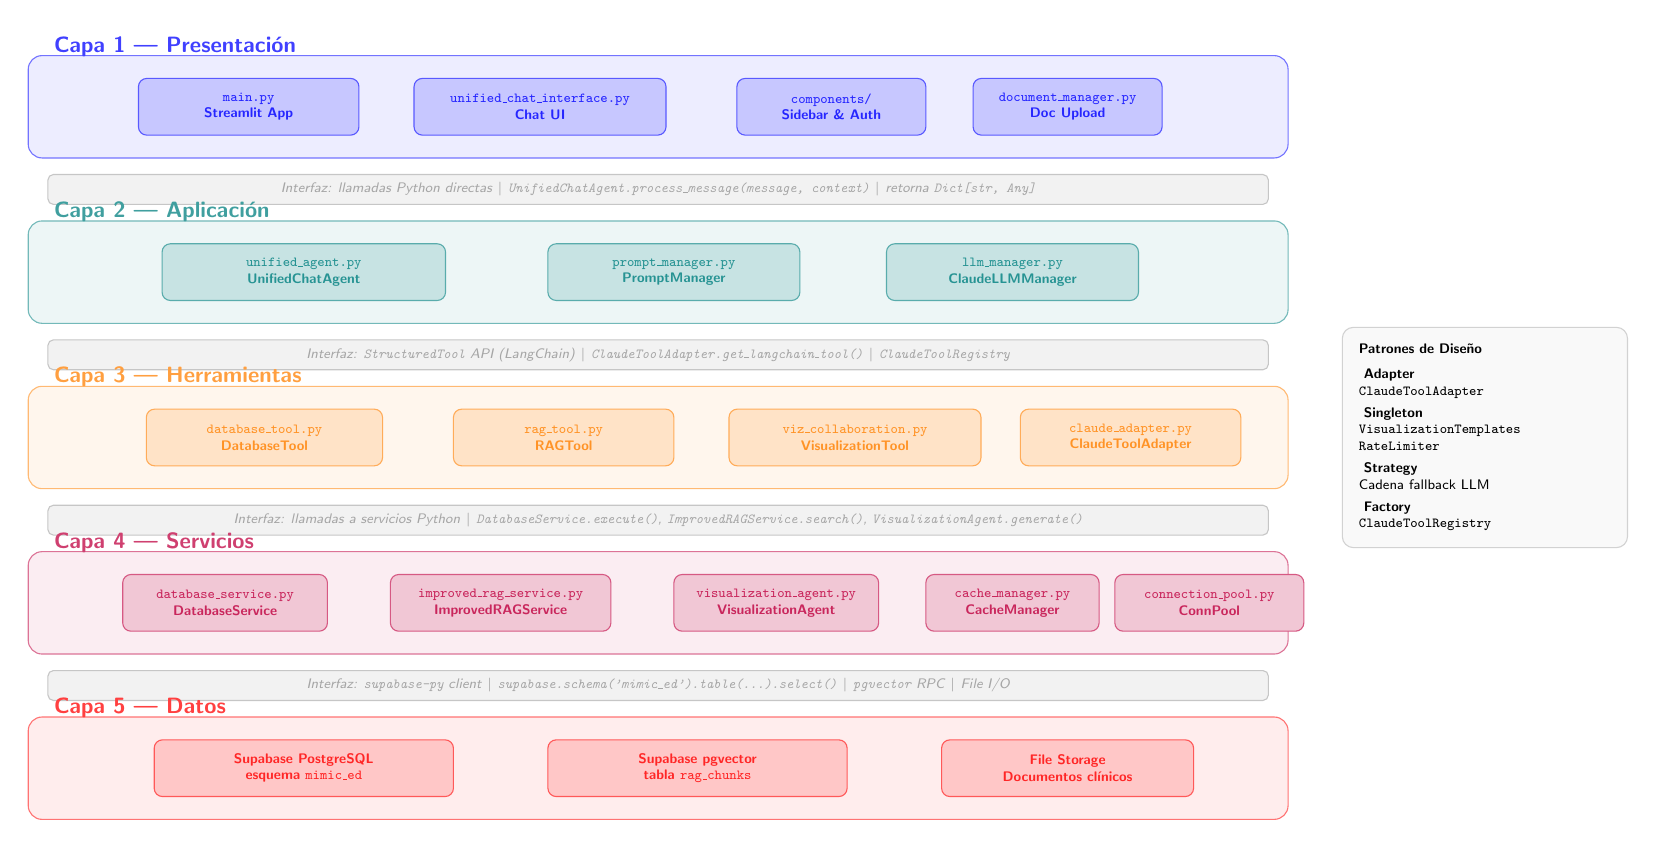
\begin{tikzpicture}[
  layerbox/.style={
    draw=#1!55, fill=#1!7, rounded corners=5pt,
    minimum width=16cm, inner sep=7pt,
    font=\footnotesize\sffamily
  },
  compbox/.style={
    draw=#1!65, fill=#1!22, rounded corners=3pt,
    minimum height=0.72cm, font=\tiny\sffamily\bfseries,
    text=#1!85, align=center, inner sep=3pt
  },
  ifacebox/.style={
    draw=gray!45, fill=gray!10, rounded corners=2pt,
    minimum height=0.38cm, font=\tiny\sffamily\itshape,
    text=gray!70, align=center, inner sep=2pt
  },
  layerlabel/.style={
    font=\footnotesize\sffamily\bfseries, text=#1!75
  },
  patternbadge/.style={
    draw=#1!60, fill=#1!15, rounded corners=8pt,
    font=\tiny\sffamily\bfseries, text=#1!80,
    inner sep=2pt, minimum height=0.35cm
  }
]

% ---- Capa 1: Presentación ----
\node[layerbox=blue, minimum height=1.3cm] (L1) at (0, 0) {};
\node[layerlabel=blue, anchor=west] at ([xshift=6pt, yshift=3pt]L1.north west) {Capa 1 — Presentación};
\node[compbox=blue, minimum width=2.8cm] at (-5.2, 0) {\texttt{main.py}\\Streamlit App};
\node[compbox=blue, minimum width=3.2cm] at (-1.5, 0) {\texttt{unified\_chat\_interface.py}\\Chat UI};
\node[compbox=blue, minimum width=2.4cm] at (2.2, 0) {\texttt{components/}\\Sidebar \& Auth};
\node[compbox=blue, minimum width=2.4cm] at (5.2, 0) {\texttt{document\_manager.py}\\Doc Upload};

% ---- Interfaz 1→2 ----
\node[ifacebox, minimum width=15.5cm] (I12) at (0, -1.05) {Interfaz: llamadas Python directas $\mid$ \texttt{UnifiedChatAgent.process\_message(message, context)} $\mid$ retorna \texttt{Dict[str, Any]}};

% ---- Capa 2: Aplicación ----
\node[layerbox=teal, minimum height=1.3cm] (L2) at (0, -2.1) {};
\node[layerlabel=teal, anchor=west] at ([xshift=6pt, yshift=3pt]L2.north west) {Capa 2 — Aplicación};
\node[compbox=teal, minimum width=3.6cm] at (-4.5, -2.1) {\texttt{unified\_agent.py}\\UnifiedChatAgent};
\node[compbox=teal, minimum width=3.2cm] at (0.2, -2.1) {\texttt{prompt\_manager.py}\\PromptManager};
\node[compbox=teal, minimum width=3.2cm] at (4.5, -2.1) {\texttt{llm\_manager.py}\\ClaudeLLMManager};

% ---- Interfaz 2→3 ----
\node[ifacebox, minimum width=15.5cm] (I23) at (0, -3.15) {Interfaz: \texttt{StructuredTool} API (LangChain) $\mid$ \texttt{ClaudeToolAdapter.get\_langchain\_tool()} $\mid$ \texttt{ClaudeToolRegistry}};

% ---- Capa 3: Herramientas ----
\node[layerbox=orange, minimum height=1.3cm] (L3) at (0, -4.2) {};
\node[layerlabel=orange, anchor=west] at ([xshift=6pt, yshift=3pt]L3.north west) {Capa 3 — Herramientas};
\node[compbox=orange, minimum width=3.0cm] at (-5.0, -4.2) {\texttt{database\_tool.py}\\DatabaseTool};
\node[compbox=orange, minimum width=2.8cm] at (-1.2, -4.2) {\texttt{rag\_tool.py}\\RAGTool};
\node[compbox=orange, minimum width=3.2cm] at (2.5, -4.2) {\texttt{viz\_collaboration.py}\\VisualizationTool};
\node[compbox=orange, minimum width=2.8cm] at (6.0, -4.2) {\texttt{claude\_adapter.py}\\ClaudeToolAdapter};

% ---- Interfaz 3→4 ----
\node[ifacebox, minimum width=15.5cm] (I34) at (0, -5.25) {Interfaz: llamadas a servicios Python $\mid$ \texttt{DatabaseService.execute()}, \texttt{ImprovedRAGService.search()}, \texttt{VisualizationAgent.generate()}};

% ---- Capa 4: Servicios ----
\node[layerbox=purple, minimum height=1.3cm] (L4) at (0, -6.3) {};
\node[layerlabel=purple, anchor=west] at ([xshift=6pt, yshift=3pt]L4.north west) {Capa 4 — Servicios};
\node[compbox=purple, minimum width=2.6cm] at (-5.5, -6.3) {\texttt{database\_service.py}\\DatabaseService};
\node[compbox=purple, minimum width=2.8cm] at (-2.0, -6.3) {\texttt{improved\_rag\_service.py}\\ImprovedRAGService};
\node[compbox=purple, minimum width=2.6cm] at (1.5, -6.3) {\texttt{visualization\_agent.py}\\VisualizationAgent};
\node[compbox=purple, minimum width=2.2cm] at (4.5, -6.3) {\texttt{cache\_manager.py}\\CacheManager};
\node[compbox=purple, minimum width=2.4cm] at (7.0, -6.3) {\texttt{connection\_pool.py}\\ConnPool};

% ---- Interfaz 4→5 ----
\node[ifacebox, minimum width=15.5cm] (I45) at (0, -7.35) {Interfaz: \texttt{supabase-py} client $\mid$ \texttt{supabase.schema('mimic\_ed').table(...).select()} $\mid$ \texttt{pgvector} RPC $\mid$ File I/O};

% ---- Capa 5: Datos ----
\node[layerbox=red, minimum height=1.3cm] (L5) at (0, -8.4) {};
\node[layerlabel=red, anchor=west] at ([xshift=6pt, yshift=3pt]L5.north west) {Capa 5 — Datos};
\node[compbox=red, minimum width=3.8cm] at (-4.5, -8.4) {Supabase PostgreSQL\\esquema \texttt{mimic\_ed}};
\node[compbox=red, minimum width=3.8cm] at (0.5, -8.4) {Supabase pgvector\\tabla \texttt{rag\_chunks}};
\node[compbox=red, minimum width=3.2cm] at (5.2, -8.4) {File Storage\\Documentos clínicos};

% ---- Leyenda de patrones (derecha) ----
\node[draw=gray!35, fill=gray!5, rounded corners=4pt, inner sep=6pt,
      font=\tiny\sffamily, align=left, text width=3.2cm] at (10.5, -4.2)
  {\textbf{Patrones de Diseño}\\[3pt]
   \textcolor{orange!80}{$\blacksquare$} \textbf{Adapter}\\
   \texttt{ClaudeToolAdapter}\\[2pt]
   \textcolor{purple!80}{$\blacksquare$} \textbf{Singleton}\\
   \texttt{VisualizationTemplates}\\
   \texttt{RateLimiter}\\[2pt]
   \textcolor{teal!80}{$\blacksquare$} \textbf{Strategy}\\
   Cadena fallback LLM\\[2pt]
   \textcolor{blue!80}{$\blacksquare$} \textbf{Factory}\\
   \texttt{ClaudeToolRegistry}};

\end{tikzpicture}
\caption{Arquitectura por capas de ChatHCE con interfaces entre capas y patrones de diseño. Las interfaces definen los contratos entre capas adyacentes; ninguna capa puede saltarse una capa intermedia para acceder a otra.}
\label{fig:capas_interfaces}
\end{figure*}

\subsubsection{Descripción de las Cinco Capas}

\textbf{Capa 1 — Presentación.} Implementada íntegramente con Streamlit, gestiona la interfaz de usuario sin contener lógica de negocio. Sus componentes son: \texttt{main.py} (punto de entrada de la aplicación), \texttt{unified\_chat\_interface.py} (interfaz de chat con renderizado de mensajes, visualizaciones y fuentes), y el directorio \texttt{components/} (sidebar de navegación, páginas de autenticación, gestor de documentos). Esta capa recibe eventos del usuario y delega todo el procesamiento a la capa de aplicación mediante llamadas Python directas. Su aislamiento permite sustituir Streamlit por otro framework de UI sin modificar ninguna capa inferior.

\textbf{Capa 2 — Aplicación.} Contiene la lógica de orquestación del sistema. El \texttt{UnifiedChatAgent} (\texttt{unified\_agent.py}) es el componente central: recibe la consulta del usuario, gestiona el historial conversacional (hasta 150K tokens), invoca el \texttt{AgentExecutor} de LangChain y sintetiza la respuesta final. El \texttt{PromptManager} (\texttt{prompt\_manager.py}) genera y cachea el prompt del sistema bajo un límite de 4000 tokens, con caché independiente por sección. El \texttt{ClaudeLLMManager} (\texttt{llm\_manager.py}) gestiona la cadena de fallback de modelos y los reintentos con backoff exponencial. Esta capa aplica el patrón \textit{Strategy} para la selección de modelos.

\textbf{Capa 3 — Herramientas.} Tres herramientas especializadas adaptadas al formato de LangChain mediante el patrón \textit{Adapter}: \texttt{DatabaseTool} (\texttt{database\_tool.py}) para consultas SQL sobre MIMIC-IV-ED, \texttt{RAGTool} (\texttt{rag\_tool.py}) para búsqueda semántica en documentos clínicos, y \texttt{VisualizationTool} (\texttt{viz\_collaboration.py}) para generación de gráficas. La clase abstracta \texttt{ClaudeToolAdapter} (\texttt{claude\_adapter.py}) define la interfaz común que todas las herramientas deben implementar, y el \texttt{ClaudeToolRegistry} aplica el patrón \textit{Factory} para su registro y recuperación centralizada.

\textbf{Capa 4 — Servicios.} Servicios de infraestructura que encapsulan el acceso a recursos externos: \texttt{DatabaseService} (\texttt{database\_service.py}) con validación SQL multicapa y decorador \texttt{@retry\_on\_failure}, \texttt{ImprovedRAGService} (\texttt{improved\_rag\_service.py}) con pipeline de búsqueda híbrida y reranking, \texttt{VisualizationAgent} (\texttt{visualization\_agent.py}) con inicialización \textit{lazy} y enfoque \textit{template-first}, \texttt{CacheManager} (\texttt{cache\_manager.py}) con política LRU y TTL configurable, y el gestor de pool de conexiones (\texttt{connection\_pool\_manager.py}). Esta capa aplica el patrón \textit{Singleton} en \texttt{VisualizationTemplates} y \texttt{RateLimiter}.

\textbf{Capa 5 — Datos.} Backend de datos unificado en Supabase: PostgreSQL con el esquema \texttt{mimic\_ed} (6 tablas MIMIC-IV-ED), Supabase pgvector con la tabla \texttt{rag\_chunks} (embeddings de 384 dimensiones con índice HNSW), y almacenamiento de archivos para documentos clínicos indexados. El acceso se realiza exclusivamente mediante el cliente Python \texttt{supabase-py}, con especificación obligatoria de esquema para tablas clínicas.

\subsubsection{Patrones de Diseño Aplicados}

\textbf{Adapter} (\texttt{ClaudeToolAdapter}). Problema: las tres herramientas del sistema tienen interfaces heterogéneas (SQL, búsqueda vectorial, generación de código), pero LangChain requiere que todas implementen la interfaz \texttt{StructuredTool}. Solución: la clase abstracta \texttt{ClaudeToolAdapter} define los métodos \texttt{execute()}, \texttt{format\_input()}, \texttt{format\_output()} y \texttt{get\_langchain\_tool()}, que cada herramienta implementa. Beneficio: añadir una nueva herramienta requiere únicamente implementar esta interfaz, sin modificar el agente.

\textbf{Singleton} (\texttt{VisualizationTemplates}, \texttt{RateLimiter}). Problema: las plantillas de visualización y el estado del rate limiter deben ser compartidos entre todas las instancias del sistema sin duplicación. Solución: ambas clases implementan el patrón Singleton con \texttt{\_instance = None} y \texttt{\_\_new\_\_} sobrescrito. Beneficio: estado compartido consistente y ahorro de memoria.

\textbf{Strategy} (cadena de fallback LLM). Problema: el modelo LLM óptimo puede variar en tiempo de ejecución según disponibilidad y carga. Solución: \texttt{ClaudeLLMManager} mantiene una lista ordenada de configuraciones de modelos (\texttt{self.models}) y el método \texttt{switch\_to\_fallback()} intercambia el algoritmo (modelo) en tiempo de ejecución sin modificar el código cliente. Beneficio: alta disponibilidad sin cambios en la lógica del agente.

\textbf{Factory} (\texttt{ClaudeToolRegistry}). Problema: la creación y registro de herramientas debe estar centralizada para facilitar la extensibilidad. Solución: el \texttt{ClaudeToolRegistry} actúa como fábrica centralizada que registra herramientas por nombre y las recupera bajo demanda. Las funciones \texttt{create\_database\_tool()}, \texttt{create\_rag\_tool()} y \texttt{create\_visualization\_collaboration\_tool()} encapsulan la lógica de construcción. Beneficio: el agente no necesita conocer los detalles de construcción de cada herramienta.

% ============================================================================
\subsection{Decisiones de Diseño Justificadas}
\label{sec:decisiones_diseno}
% ============================================================================

Esta sección documenta las cinco decisiones arquitectónicas más relevantes de ChatHCE siguiendo el formato \textit{Architecture Decision Record} (ADR) \citep{Nygard2011}: \textbf{[Problema]} $\rightarrow$ \textbf{[Alternativas]} $\rightarrow$ \textbf{[Decisión]} $\rightarrow$ \textbf{[Justificación]}. Este formato garantiza que las decisiones sean trazables, reproducibles y auditables, demostrando que no fueron arbitrarias sino el resultado de un análisis razonado de alternativas.

% ---- Decisión 1 ----
\begin{tcolorbox}[
  enhanced, breakable,
  colback=blue!4, colframe=blue!45,
  title={\footnotesize\sffamily\bfseries Decisión 1 — Supabase como backend unificado (vs.\ servicios separados)},
  fonttitle=\color{white},
  attach boxed title to top left={yshift=-2mm, xshift=4mm},
  boxed title style={colback=blue!55, rounded corners},
  left=4pt, right=4pt, top=4pt, bottom=4pt
]
\footnotesize
\textbf{Problema:} El sistema requiere simultáneamente almacenamiento relacional (datos MIMIC-IV-ED), almacén vectorial (embeddings RAG), autenticación de usuarios y API REST. Gestionar tres o cuatro servicios independientes introduce complejidad operacional y latencia de red entre ellos.

\textbf{Alternativas consideradas:}
\begin{itemize}[nosep, leftmargin=*]
  \item PostgreSQL + Pinecone + Auth0 (tres servicios separados, tres SDKs, tres puntos de fallo)
  \item MongoDB Atlas + Weaviate (sin soporte SQL nativo, sin búsqueda híbrida integrada)
  \item Firebase + Chroma (sin PostgreSQL completo, sin funciones de ventana para análisis temporal)
\end{itemize}

\textbf{Decisión adoptada:} Supabase (PostgreSQL 15 + pgvector 0.8.0 + Supabase Auth).

\textbf{Justificación técnica:} La búsqueda híbrida vectorial-léxica se ejecuta como una única función RPC de PostgreSQL, eliminando la latencia de red entre un servicio vectorial externo y la base de datos relacional. Un solo punto de autenticación con Row Level Security (RLS) aplica políticas de acceso uniformes sobre las 13 tablas del sistema. PostgREST genera automáticamente la API REST sin código adicional. La superficie de ataque se reduce a un único servicio frente a tres con sus propias vulnerabilidades y configuraciones de seguridad independientes. Evidencia en código: \texttt{services/medical\_agent/services/database\_service.py} accede a ambos esquemas (\texttt{mimic\_ed} y \texttt{public}) mediante el mismo cliente \texttt{supabase-py}, y la función RPC \texttt{hybrid\_search} en \texttt{services/rag/supabase\_vector\_store.py} combina pgvector y tsvector en una sola llamada.
\end{tcolorbox}

% ---- Decisión 2 ----
\begin{tcolorbox}[
  enhanced, breakable,
  colback=teal!4, colframe=teal!45,
  title={\footnotesize\sffamily\bfseries Decisión 2 — Chunking jerárquico padre-hijo (vs.\ chunking uniforme)},
  fonttitle=\color{white},
  attach boxed title to top left={yshift=-2mm, xshift=4mm},
  boxed title style={colback=teal!55, rounded corners},
  left=4pt, right=4pt, top=4pt, bottom=4pt
]
\footnotesize
\textbf{Problema:} Existe un \textit{trade-off} fundamental en RAG entre granularidad para búsqueda precisa y contexto suficiente para generación de respuestas. Los chunks pequeños mejoran la precisión de recuperación pero truncan el contexto clínico; los chunks grandes preservan el contexto pero degradan la precisión semántica.

\textbf{Alternativas consideradas:}
\begin{itemize}[nosep, leftmargin=*]
  \item Chunking fijo de 512 tokens (estándar, pero pierde contexto en guías con dosis y protocolos)
  \item Chunking por párrafo (tamaño variable, difícil de controlar)
  \item Chunking por oración (demasiado granular para embeddings de 384 dimensiones)
\end{itemize}

\textbf{Decisión adoptada:} Chunks hijo de 400 caracteres para búsqueda + expansión a chunks padre de 1500 caracteres para contexto, implementado en \texttt{services/rag/parent\_child\_chunker.py}.

\textbf{Justificación técnica:} Los bi-encoders de 384 dimensiones como \texttt{all-MiniLM-L6-v2} capturan mejor la semántica en fragmentos cortos \citep{Wang2020}. La expansión al chunk padre garantiza que el LLM recibe contexto clínico completo sin truncar oraciones a mitad, especialmente relevante para guías con dosificaciones y protocolos de urgencias donde la continuidad del texto es crítica. La columna \texttt{parent\_id} en \texttt{rag\_chunks} implementa la expansión con una sola query SQL JOIN, sin overhead adicional. Los parámetros \texttt{CHILD\_CHUNK\_SIZE = 400} y \texttt{PARENT\_CHUNK\_SIZE = 1500} están configurados en \texttt{services/rag/parent\_child\_chunker.py}.
\end{tcolorbox}

% ---- Decisión 3 ----
\begin{tcolorbox}[
  enhanced, breakable,
  colback=purple!4, colframe=purple!45,
  title={\footnotesize\sffamily\bfseries Decisión 3 — Búsqueda híbrida vectorial-léxica con RRF (vs.\ búsqueda vectorial pura)},
  fonttitle=\color{white},
  attach boxed title to top left={yshift=-2mm, xshift=4mm},
  boxed title style={colback=purple!55, rounded corners},
  left=4pt, right=4pt, top=4pt, bottom=4pt
]
\footnotesize
\textbf{Problema:} La búsqueda vectorial pura falla en términos médicos exactos. Códigos ICD como \texttt{I48.91} (fibrilación auricular), nombres de fármacos como \texttt{metoprolol 25mg} o dosificaciones específicas no tienen buena cobertura semántica en embeddings genéricos entrenados sobre texto general.

\textbf{Alternativas consideradas:}
\begin{itemize}[nosep, leftmargin=*]
  \item Búsqueda vectorial pura (similitud coseno): falla en términos exactos y acrónimos médicos
  \item BM25 pura: no captura sinónimos ni variantes semánticas
  \item ElasticSearch: servicio externo adicional, latencia de red, coste operacional
\end{itemize}

\textbf{Decisión adoptada:} pgvector (similitud coseno) + tsvector (full-text search en español) + Reciprocal Rank Fusion (RRF), ejecutado como función RPC en PostgreSQL.

\textbf{Justificación técnica:} La búsqueda léxica con stemming en español (\texttt{tsvector} con configuración \texttt{spanish}) mejora el recall para variantes morfológicas de términos médicos. RRF combina los rankings de ambas búsquedas sin requerir calibración de pesos, usando la fórmula $\text{RRF}(d) = \sum_{r \in R} \frac{1}{k + r(d)}$ con $k=60$ \citep{Cormack2009}. Todo se ejecuta como función RPC de PostgreSQL, con latencia media medida inferior a 500 ms. Evidencia en código: función \texttt{hybrid\_search} en \texttt{services/rag/supabase\_vector\_store.py} y columna generada \texttt{fts tsvector} en la tabla \texttt{rag\_chunks}.
\end{tcolorbox}

% ---- Decisión 4 ----
\begin{tcolorbox}[
  enhanced, breakable,
  colback=orange!4, colframe=orange!45,
  title={\footnotesize\sffamily\bfseries Decisión 4 — Enfoque template-first en visualización (vs.\ generación LLM para todo)},
  fonttitle=\color{white},
  attach boxed title to top left={yshift=-2mm, xshift=4mm},
  boxed title style={colback=orange!55, rounded corners},
  left=4pt, right=4pt, top=4pt, bottom=4pt
]
\footnotesize
\textbf{Problema:} La generación de código Plotly por LLM introduce latencia de $\sim$4 segundos y no-determinismo: el mismo tipo de gráfica puede producir código diferente en cada invocación, con riesgo de errores de ejecución.

\textbf{Alternativas consideradas:}
\begin{itemize}[nosep, leftmargin=*]
  \item LLM para todos los casos: máxima flexibilidad pero latencia alta y no-determinismo
  \item Librería predefinida sin LLM: latencia mínima pero sin flexibilidad para casos atípicos
\end{itemize}

\textbf{Decisión adoptada:} 12+ plantillas Plotly predefinidas en \texttt{VisualizationTemplates} (Singleton) + fallback a Claude Sonnet 4.5 (\texttt{claude-sonnet-4-5}) para casos no cubiertos.

\textbf{Justificación técnica:} Las visualizaciones clínicas habituales son predecibles: timeline de signos vitales, distribuciones de diagnósticos, comparativas entre pacientes, indicadores de triaje. Las plantillas reducen la latencia de $\sim$4 s a $\sim$0.4 s en el 90\% de los casos. El fallback al LLM garantiza flexibilidad para visualizaciones atípicas. La inicialización \textit{lazy} del \texttt{VisualizationAgent} (\texttt{services/medical\_agent/visualization\_agent.py}) ahorra memoria en el 90\% de las consultas que no requieren generación LLM. El \texttt{VisualizationSelector} (\texttt{services/medical\_agent/visualization\_selector.py}) analiza las características de los datos (tipos de columnas, cardinalidad, presencia de series temporales) para seleccionar automáticamente la plantilla apropiada.
\end{tcolorbox}

% ---- Decisión 5 (Central) ----
\begin{tcolorbox}[
  enhanced, breakable,
  colback=orange!6, colframe=orange!60,
  title={\small\sffamily\bfseries\color{white} Decisión Arquitectónica Central — Agente Unificado vs.\ Arquitectura Multi-Agente},
  attach boxed title to top left={yshift=-2mm, xshift=4mm},
  boxed title style={colback=orange!70, rounded corners},
  left=5pt, right=5pt, top=5pt, bottom=5pt
]
\footnotesize
\textbf{Problema:} Elegir entre un agente conversacional unificado y una arquitectura multi-agente con agentes especializados para cada dominio (base de datos, RAG, visualización, crítica).

\textbf{Alternativas consideradas:}
\begin{itemize}[nosep, leftmargin=*]
  \item \textbf{Multi-agente con LangGraph}: grafo DAG con \texttt{OrchestratorAgent} $\rightarrow$ [\texttt{DBAgent}, \texttt{RAGAgent}, \texttt{VizAgent}] $\rightarrow$ \texttt{CriticAgent}. Mayor paralelización pero latencia acumulada y error propagado entre nodos.
  \item \textbf{Multi-agente con CrewAI}: roles especializados (médico, buscador, crítico). Mayor expresividad semántica pero complejidad de coordinación y coste de múltiples llamadas LLM por turno.
  \item \textbf{Agente único sin herramientas}: prompt gigante sin tool-calling. Sin latencia de coordinación pero sin acceso a datos reales, inaceptable para un sistema clínico.
\end{itemize}

\textbf{Decisión adoptada:} Agente unificado (\texttt{UnifiedChatAgent}) con tool-calling nativo de Claude Haiku 4.5, implementado en \texttt{services/unified\_chat/unified\_agent.py}.

\textbf{Justificación técnica:}
\begin{itemize}[nosep, leftmargin=*]
  \item \textbf{Menor latencia}: una sola llamada LLM por turno de conversación frente a 3-5 llamadas en arquitecturas multi-agente. El \texttt{AgentExecutor} con \texttt{max\_iterations=5} y \texttt{max\_execution\_time=120} garantiza un límite superior de tiempo.
  \item \textbf{Menor error acumulado}: en cadenas de agentes, cada paso puede propagar errores o malinterpretaciones. El agente unificado sintetiza directamente desde los resultados de las herramientas.
  \item \textbf{Capacidad suficiente}: Claude Haiku 4.5 tiene capacidad de razonamiento clínico suficiente para el 95\% de las consultas, como demuestran los resultados de los test cases de evaluación (Sección~\ref{sec:evaluacion}).
  \item \textbf{Tool-calling determinista}: Claude genera directamente el nombre de la herramienta y los parámetros en JSON, sin simulación mediante prompts. El método \texttt{create\_tool\_calling\_agent(llm, tools, prompt)} de LangChain aprovecha esta capacidad nativa.
  \item \textbf{Fallback elegante}: la cadena Haiku $\rightarrow$ Sonnet $\rightarrow$ Opus proporciona la escalabilidad que normalmente se busca con multi-agente, pero con menor complejidad arquitectónica.
\end{itemize}

\textbf{Trade-offs asumidos:} Se pierde la paralelización de agentes (mitigado porque las herramientas son rápidas: P50 $<$ 2 s) y la revisión crítica autónoma (mitigado por las directivas anti-alucinación en el prompt del sistema, Sección~\ref{sec:antihallucination_37}).
\end{tcolorbox}

La Figura~\ref{fig:agente_vs_multiagente} ilustra visualmente la comparativa entre la arquitectura multi-agente descartada y el agente unificado adoptado.

\begin{figure*}[t]
\centering
\begin{tikzpicture}[
  agentnode/.style={
    draw=#1!65, fill=#1!12, rounded corners=4pt,
    minimum width=2.6cm, minimum height=0.7cm,
    font=\small\sffamily, text=#1!80, align=center
  },
  toolnode/.style={
    draw=#1!60, fill=#1!18, rounded corners=3pt,
    minimum width=2.2cm, minimum height=0.6cm,
    font=\small\sffamily\bfseries, text=#1!80, align=center
  },
  disadvlabel/.style={
    font=\tiny\sffamily\itshape, text=accent!70, align=center
  },
  advlabel/.style={
    font=\tiny\sffamily\itshape, text=success!70, align=center
  },
  flowarrow/.style={
    -{Stealth[length=5pt]}, thick, color=#1!60
  }
]

% ===== COLUMNA IZQUIERDA: Multi-Agente (descartado) =====
\node[font=\small\sffamily\bfseries, text=gray!60] at (-5.5, 4.5) {Arquitectura Multi-Agente};
\node[font=\tiny\sffamily\itshape, text=gray!50] at (-5.5, 4.1) {(alternativa descartada)};

\node[agentnode=gray, minimum width=3.0cm] (orch) at (-5.5, 3.2) {OrchestratorAgent};
\node[agentnode=gray, minimum width=2.4cm] (dba) at (-7.5, 1.8) {DBAgent};
\node[agentnode=gray, minimum width=2.4cm] (raga) at (-5.5, 1.8) {RAGAgent};
\node[agentnode=gray, minimum width=2.4cm] (viza) at (-3.5, 1.8) {VizAgent};
\node[agentnode=gray, minimum width=3.0cm] (critic) at (-5.5, 0.4) {CriticAgent};
\node[agentnode=gray, minimum width=3.0cm] (resp1) at (-5.5, -0.8) {Respuesta};

\draw[flowarrow=gray] (orch) -- (dba);
\draw[flowarrow=gray] (orch) -- (raga);
\draw[flowarrow=gray] (orch) -- (viza);
\draw[flowarrow=gray] (dba) |- (critic);
\draw[flowarrow=gray] (raga) -- (critic);
\draw[flowarrow=gray] (viza) |- (critic);
\draw[flowarrow=gray] (critic) -- (resp1);

% Etiquetas de desventajas
\node[disadvlabel] at (-5.5, -1.5) {$\times$ 3--5 llamadas LLM por turno};
\node[disadvlabel] at (-5.5, -1.9) {$\times$ Error acumulado entre nodos};
\node[disadvlabel] at (-5.5, -2.3) {$\times$ Complejidad de coordinación};
\node[disadvlabel] at (-5.5, -2.7) {$\times$ Latencia $>$ 10 s (estimada)};

% Cruz roja
\node[font=\Large\bfseries, text=accent] at (-5.5, 5.0) {$\times$};

% ===== SEPARADOR CENTRAL =====
\draw[very thick, gray!30, dashed] (0, -3.2) -- (0, 5.2);
\node[font=\large\sffamily\bfseries, text=gray!50] at (0, 1.2) {vs.};

% ===== COLUMNA DERECHA: Agente Unificado (adoptado) =====
\node[font=\small\sffamily\bfseries, text=success!70] at (5.5, 4.5) {Agente Unificado ChatHCE};
\node[font=\tiny\sffamily\itshape, text=success!50] at (5.5, 4.1) {(decisión adoptada)};

\node[agentnode=success, minimum width=3.8cm] (unified) at (5.5, 3.2) {UnifiedChatAgent\\Claude Haiku 4.5};

\node[toolnode=dbcolor, minimum width=2.2cm] (dbt) at (3.5, 1.8) {DB Tool};
\node[toolnode=ragcolor, minimum width=2.2cm] (ragt) at (5.5, 1.8) {RAG Tool};
\node[toolnode=vizcolor, minimum width=2.2cm] (vizt) at (7.5, 1.8) {VIZ Tool};

\node[agentnode=success, minimum width=3.8cm] (synth) at (5.5, 0.4) {Síntesis directa\\(una sola llamada LLM)};
\node[agentnode=success, minimum width=3.8cm] (resp2) at (5.5, -0.8) {Respuesta integrada};

\draw[flowarrow=success] (unified) -- (dbt);
\draw[flowarrow=success] (unified) -- (ragt);
\draw[flowarrow=success] (unified) -- (vizt);
\draw[flowarrow=dbcolor] (dbt) |- (synth);
\draw[flowarrow=ragcolor] (ragt) -- (synth);
\draw[flowarrow=vizcolor] (vizt) |- (synth);
\draw[flowarrow=success] (synth) -- (resp2);

% Cadena de fallback
\node[draw=accent!50, fill=accent!8, rounded corners=3pt,
      font=\tiny\sffamily, align=center, inner sep=3pt,
      minimum width=2.8cm] (fallback) at (9.5, 3.2)
  {Fallback:\\Haiku $\rightarrow$ Sonnet\\$\rightarrow$ Opus};
\draw[dashedarrow, color=accent!50] (unified.east) -- (fallback.west);

% Etiquetas de ventajas
\node[advlabel] at (5.5, -1.5) {$\checkmark$ 1 llamada LLM por turno};
\node[advlabel] at (5.5, -1.9) {$\checkmark$ Sin error acumulado};
\node[advlabel] at (5.5, -2.3) {$\checkmark$ Fallback elegante integrado};
\node[advlabel] at (5.5, -2.7) {$\checkmark$ Latencia P50 $<$ 5 s (medida)};

% Check verde
\node[font=\Large\bfseries, text=success] at (5.5, 5.0) {$\checkmark$};

\end{tikzpicture}
\caption{Comparativa entre la arquitectura multi-agente descartada (izquierda) y el agente unificado adoptado (derecha). El agente unificado reduce la latencia, elimina el error acumulado entre nodos y simplifica la arquitectura sin sacrificar capacidad de razonamiento clínico.}
\label{fig:agente_vs_multiagente}
\end{figure*}

% ============================================================================
\subsection{Arquitectura del Agente y Selección de Herramientas}
\label{sec:arquitectura_agente}
% ============================================================================

\subsubsection{El Ciclo ReAct del Agente}
\label{sec:react}

El \texttt{UnifiedChatAgent} implementa el patrón \textbf{ReAct} (\textit{Reasoning + Acting}) \citep{Yao2022}, que intercala razonamiento en lenguaje natural con acciones concretas sobre herramientas externas. A diferencia de los enfoques que separan el razonamiento de la acción, ReAct permite que el modelo actualice su plan de acción en función de las observaciones obtenidas de las herramientas, produciendo respuestas más precisas y fundamentadas en datos reales.

El ciclo ReAct en ChatHCE se articula en cuatro fases iterativas, gestionadas por el \texttt{AgentExecutor} de LangChain con \texttt{max\_iterations=5} y \texttt{max\_execution\_time=120} segundos:

\begin{enumerate}[nosep, leftmargin=*]
  \item \textbf{Think}: Claude Haiku 4.5 analiza la consulta del usuario, el historial conversacional y el contexto de datos previos inyectado por \texttt{\_enrich\_message\_with\_context()}. Determina qué herramientas invocar y con qué parámetros.
  \item \textbf{Act}: El modelo genera directamente el nombre de la herramienta y los parámetros en JSON mediante tool-calling nativo (no simulado con prompts). La función \texttt{create\_tool\_calling\_agent(llm, tools, prompt)} de LangChain aprovecha esta capacidad nativa de Claude.
  \item \textbf{Observe}: El \texttt{AgentExecutor} ejecuta la herramienta seleccionada y devuelve el resultado al modelo. Los resultados intermedios se almacenan en \texttt{return\_intermediate\_steps=True} para trazabilidad.
  \item \textbf{Synthesize}: Claude integra los resultados de todas las herramientas invocadas y genera la respuesta final en español, con citación de fuentes y reconocimiento explícito de incertidumbre según las directivas anti-alucinación.
\end{enumerate}

La Figura~\ref{fig:react_cycle} muestra el ciclo interno completo del agente con las tres herramientas y la cadena de fallback.

\subsubsection{Las Tres Herramientas Especializadas}
\label{sec:herramientas}

\textbf{DatabaseTool} (\texttt{query\_mimic\_database}). Recibe una consulta en lenguaje natural que el agente traduce a parámetros estructurados según el esquema Pydantic \texttt{DatabaseToolInput}. Los campos del esquema son: \texttt{query\_type} (tipos: \texttt{patient\_summary}, \texttt{vital\_signs}, \texttt{diagnoses}, \texttt{medications}, \texttt{custom}), \texttt{subject\_id} (INT, opcional), \texttt{stay\_id} (INT, opcional), \texttt{icd\_code} (VARCHAR, opcional), \texttt{custom\_query} (SQL validado, opcional) y \texttt{limit} (INT, máximo 5000, por defecto 1000). La herramienta delega en \texttt{DatabaseService} para la ejecución, aplicando validación SQL multicapa antes de cada consulta. Retorna un \texttt{Dict} con \texttt{success}, \texttt{data}, \texttt{query\_type}, \texttt{parameters} y \texttt{count}.

\textbf{RAGTool} (\texttt{search\_clinical\_documents}). Recibe una consulta clínica en lenguaje natural. Internamente, el \texttt{QueryAugmenter} genera hasta 3 consultas alternativas mediante Multi-Query y HyDE (Hypothetical Document Embeddings) \citep{Gao2022}. La búsqueda híbrida recupera los $k$ chunks más relevantes (por defecto $k=5$) con sus puntuaciones de similitud $s_i \in [0,1]$. El \texttt{Reranker} reordena los resultados con \texttt{cross-encoder/ms-marco-MiniLM-L-6-v2}. Retorna los chunks con metadatos de fuente (\texttt{filename}, \texttt{specialty}, \texttt{document\_type}) para citación obligatoria.

\textbf{VisualizationTool} (\texttt{request\_visualization}). Recibe los datos clínicos y el tipo de gráfica solicitado. El \texttt{DataPreprocessor} limpia y valida los datos (máximo 5000 puntos). El \texttt{VisualizationSelector} selecciona la plantilla apropiada entre 12+ tipos: \texttt{timeline}, \texttt{comparison}, \texttt{histogram}, \texttt{scatter}, \texttt{bar}, \texttt{box}, \texttt{violin}, \texttt{heatmap}, \texttt{pie}, \texttt{sunburst}, \texttt{table} e \texttt{indicator}. Si no existe plantilla adecuada, el \texttt{VisualizationAgent} (inicialización \textit{lazy}) genera código Python con Claude Sonnet 4.5. El \texttt{CodeValidator} valida el código mediante AST antes de la ejecución en sandbox. Retorna la figura en formato base64 PNG o HTML interactivo. En caso de error, la herramienta retorna un mensaje descriptivo sin interrumpir el flujo conversacional.

\subsubsection{La Cadena de Fallback de Modelos}
\label{sec:fallback}

El \texttt{ClaudeLLMManager} implementa una cadena de fallback con tres modelos Claude, configurada en \texttt{config/settings.py} mediante \texttt{ClaudeAgentSettings}:

\begin{itemize}[nosep, leftmargin=*]
  \item \textbf{Modelo primario}: \texttt{claude-haiku-4-5-20251001} — optimizado para velocidad y coste. Parámetros: \texttt{max\_tokens=4096}, \texttt{temperature=0.1}, \texttt{timeout=30 s}.
  \item \textbf{Modelo secundario}: \texttt{claude-sonnet-4-5-20250929} — mayor capacidad de razonamiento. Parámetros: \texttt{max\_tokens=8192}, \texttt{timeout=45 s}.
  \item \textbf{Modelo terciario}: \texttt{claude-opus-4-20250514} — máxima capacidad. Parámetros: \texttt{max\_tokens=4096}, \texttt{timeout=60 s}.
\end{itemize}

El escalado se dispara ante excepciones \texttt{AnthropicRateLimitError} o \texttt{APIError} tras agotar los reintentos del modelo actual. Los parámetros de backoff exponencial son: \texttt{max\_retries=3}, \texttt{retry\_delay=2.0 s}, \texttt{backoff\_multiplier=2.0} (delays: 2 s, 4 s, 8 s). El método \texttt{execute\_with\_retry()} en \texttt{llm\_manager.py} implementa esta lógica, intentando el fallback solo en el último reintento para minimizar la latencia en condiciones normales.

Claude Haiku 4.5 es el modelo primario por su balance entre velocidad ($\sim$800 ms P50 para análisis de intención), coste y capacidad de tool-calling nativo. La temperatura de 0.1 garantiza respuestas deterministas y reproducibles, crítico en un entorno clínico donde la consistencia es prioritaria.

\subsubsection{El Sistema de Prompts y Directivas Anti-Alucinación}
\label{sec:antihallucination_37}

El \texttt{PromptManager} genera el prompt del sistema bajo un límite de 4000 tokens, estructurado en diez secciones con caché independiente por sección (atributos \texttt{schema\_cache}, \texttt{tool\_descriptions\_cache}, \texttt{role\_definition\_cache}, \texttt{response\_format\_cache}, \texttt{clinical\_guidelines\_cache}, \texttt{anti\_hallucination\_cache}, \texttt{full\_prompt\_cache}):

\begin{enumerate}[nosep, leftmargin=*]
  \item \textbf{IDENTIDAD DEL SISTEMA}: rol de ChatHCE y propósito clínico
  \item \textbf{CONTEXTO OPERATIVO}: descripción del dataset MIMIC-IV-ED (222 pacientes, 6 tablas)
  \item \textbf{HERRAMIENTAS DISPONIBLES}: documentación de las tres herramientas con ejemplos
  \item \textbf{DIRECTIVAS ANTI-ALUCINACIÓN}: prohibiciones absolutas y manejo de datos faltantes
  \item \textbf{IDIOMA Y TERMINOLOGÍA}: directivas de respuesta en español médico
  \item \textbf{Base de Datos MIMIC-IV-ED}: esquema condensado con columnas exactas y porcentajes de nulos
  \item \textbf{Herramientas Disponibles}: descripciones detalladas con reglas SQL obligatorias
  \item \textbf{Formato de Respuesta}: estructura recomendada y convenciones de unidades
  \item \textbf{Guías Clínicas}: valores de referencia de signos vitales y niveles de acuidad ESI
  \item \textbf{GUÍAS DE SELECCIÓN DE HERRAMIENTAS}: patrones de detección automática de visualizaciones
\end{enumerate}

Las directivas anti-alucinación (sección 4 del prompt) son la capa de defensa más temprana contra la generación de información clínica falsa. Su implementación en el prompt del sistema, en lugar de como post-procesamiento, es más eficiente: interceptar antes de generar es computacionalmente más barato y más fiable que corregir después de generar. El siguiente bloque reproduce literalmente el núcleo de las directivas, obtenido del método \texttt{get\_anti\_hallucination\_directives()} en \texttt{services/medical\_agent/prompt\_manager.py}:

\begin{tcolorbox}[
  enhanced, breakable,
  colback=accent!4, colframe=accent!50,
  title={\footnotesize\sffamily\bfseries\color{white} Directivas Anti-Alucinación — Extracto del Prompt del Sistema},
  attach boxed title to top left={yshift=-2mm, xshift=4mm},
  boxed title style={colback=accent!60, rounded corners},
  left=4pt, right=4pt, top=4pt, bottom=4pt
]
\begin{lstlisting}[basicstyle=\ttfamily\tiny, backgroundcolor=\color{codebg},
  frame=none, breaklines=true, columns=fullflexible]
# DIRECTIVAS ANTI-ALUCINACION

## PROHIBICIONES ABSOLUTAS - NUNCA HACER

### Identificadores de Pacientes
- NUNCA inventes subject_id (IDs de pacientes)
- NUNCA fabriques stay_id (IDs de estancias)
- NUNCA crees hadm_id (IDs de admision hospitalaria)
- Solo usa identificadores obtenidos de una consulta real a la base de datos

### Valores Clinicos
- NUNCA inventes valores de signos vitales (temperatura, frecuencia cardiaca,
  presion arterial, saturacion O2, frecuencia respiratoria)
- NUNCA fabriques resultados de laboratorio
- Todos los valores numericos deben provenir de consultas reales

### Diagnosticos y Medicamentos
- NUNCA inventes diagnosticos o codigos ICD (ICD-9 o ICD-10)
- NUNCA fabriques nombres de medicamentos
- NUNCA crees dosis o frecuencias de administracion ficticias

## MANEJO DE DATOS FALTANTES
- Si no encuentra datos: "No encontre informacion sobre [X] en el dataset"
- Si hay valores NULL: "Algunos registros tienen datos incompletos para [campo]"
- Si el paciente no existe: "El paciente [ID] no existe en MIMIC-IV-ED"

## CITACION DE FUENTES
- Siempre indica: "Segun los datos obtenidos de la tabla [nombre_tabla]..."
- Cita el documento fuente: "Segun [nombre del documento]..."

## RECONOCIMIENTO DE INCERTIDUMBRE
- Para datos verificados: "Segun los datos disponibles..." / "Los registros muestran..."
- Para interpretaciones: "Esto podria indicar..." / "Una posible interpretacion es..."
- Para inferencias: "Analizando los datos disponibles..."
\end{lstlisting}
\end{tcolorbox}

Las directivas cubren cinco dimensiones complementarias: (1) prohibiciones absolutas de fabricación de identificadores y valores clínicos, (2) protocolos para datos faltantes o nulos, (3) citación obligatoria de fuentes con indicación de tabla y herramienta, (4) diferenciación entre datos verificados e interpretaciones mediante lenguaje condicional, y (5) recordatorio de las limitaciones del dataset (222 pacientes, solo urgencias, fechas desplazadas para anonimización).

\subsubsection{Gestión de Memoria Conversacional}
\label{sec:memoria}

El \texttt{UnifiedChatAgent} gestiona el contexto conversacional con tres mecanismos complementarios:

\textbf{Límite de tokens}: El historial se limita a \texttt{MAX\_HISTORY\_TOKENS = 150\,000} tokens (estimados como $\lfloor\text{chars}/4\rfloor$), reservando espacio para el prompt del sistema ($\sim$10K tokens) y la respuesta ($\sim$4K tokens) dentro del límite de 200K tokens de Claude. Cuando se supera el límite, se eliminan los mensajes más antiguos preservando siempre los \texttt{MIN\_MESSAGES\_TO\_KEEP = 4} mensajes más recientes.

\textbf{Inyección de contexto de datos}: El método \texttt{\_enrich\_message\_with\_context()} añade bloques \texttt{[CONTEXTO DE DATOS]} a los mensajes del asistente, con resúmenes de los resultados de herramientas de interacciones previas. Esto permite al agente referenciar datos consultados anteriormente sin re-ejecutar herramientas, mejorando la eficiencia y la coherencia conversacional. Los mensajes recientes (últimos 3) reciben contexto completo; los mensajes más antiguos reciben solo resúmenes.

\textbf{Trade-off coste-calidad}: Un historial mayor permite consultas de seguimiento más inteligentes (``¿cuál era su presión arterial?'' sin re-ejecutar la herramienta), pero aumenta el coste por token. El límite de 150K tokens representa un equilibrio entre capacidad conversacional y coste operacional, suficiente para conversaciones de hasta $\sim$50 turnos con datos clínicos completos.

% ---- Figura 3.X: Ciclo ReAct del agente ----
\begin{figure*}[t]
\centering
\begin{tikzpicture}[
  phasenode/.style={
    draw=#1!70, fill=#1!14, rounded corners=5pt,
    minimum width=3.2cm, minimum height=1.0cm,
    font=\small\sffamily\bfseries, text=#1!80, align=center,
    drop shadow={shadow xshift=1.5pt, shadow yshift=-1.5pt, fill=#1!20, opacity=0.4}
  },
  toolnode/.style={
    draw=#1!65, fill=#1!18, rounded corners=3pt,
    minimum width=2.6cm, minimum height=0.65cm,
    font=\small\sffamily\bfseries, text=#1!80, align=center
  },
  resultnode/.style={
    draw=#1!55, fill=#1!10, rounded corners=3pt,
    minimum width=2.6cm, minimum height=0.55cm,
    font=\tiny\sffamily, text=#1!75, align=center
  },
  modelnode/.style={
    draw=primary!70, fill=primary!12, rounded corners=6pt,
    minimum width=3.8cm, minimum height=1.4cm,
    font=\small\sffamily\bfseries, text=primary!80, align=center,
    drop shadow={shadow xshift=2pt, shadow yshift=-2pt, fill=primary!20, opacity=0.4}
  },
  fallbacknode/.style={
    draw=accent!55, fill=accent!8, rounded corners=3pt,
    minimum width=2.8cm, minimum height=0.55cm,
    font=\tiny\sffamily, text=accent!75, align=center
  },
  cyclearrow/.style={
    -{Stealth[length=6pt,width=4pt]}, very thick, color=#1!65
  },
  limitlabel/.style={
    draw=gray!35, fill=gray!8, rounded corners=2pt,
    font=\tiny\sffamily\itshape, text=gray!65, inner sep=2pt
  }
]

% ---- Nodo central: Claude Haiku 4.5 ----
\node[modelnode] (claude) at (0, 0) {Claude Haiku 4.5\\(\texttt{claude-haiku-4-5-20251001})\\AgentExecutor};

% ---- Fase THINK (arriba) ----
\node[phasenode=blue] (think) at (0, 3.5) {THINK\\Analiza consulta\\+ historial};
\node[limitlabel] at (3.8, 3.5) {\texttt{max\_iterations=5}\\timeout: 120 s};

% ---- Fase ACT (derecha) ----
\node[phasenode=orange] (act) at (5.5, 0) {ACT\\Tool-calling\\nativo JSON};

% ---- Fase OBSERVE (abajo) ----
\node[phasenode=purple] (observe) at (0, -3.5) {OBSERVE\\Recibe resultados\\de herramientas};

% ---- Fase SYNTHESIZE (izquierda) ----
\node[phasenode=success] (synth) at (-5.5, 0) {SYNTHESIZE\\Integra resultados\\Genera respuesta};

% ---- Flechas del ciclo ----
\draw[cyclearrow=blue] (claude.north) -- (think.south)
  node[midway, right, font=\tiny\sffamily\itshape, text=blue!60] {analiza};
\draw[cyclearrow=orange] (think.east) -- ++(1.5,0) |- (act.north)
  node[near start, above, font=\tiny\sffamily\itshape, text=orange!60] {decide herramientas};
\draw[cyclearrow=orange] (act.south) -- ++(0,-1.0) -| (observe.east)
  node[near start, right, font=\tiny\sffamily\itshape, text=orange!60] {ejecuta};
\draw[cyclearrow=purple] (observe.west) -- ++(-1.5,0) |- (synth.south)
  node[near start, below, font=\tiny\sffamily\itshape, text=purple!60] {resultados};
\draw[cyclearrow=success] (synth.north) -- ++(0,1.0) -| (claude.west)
  node[near start, left, font=\tiny\sffamily\itshape, text=success!60] {respuesta final};

% Flecha de retorno al THINK (nueva iteración)
\draw[cyclearrow=blue, dashed] (synth.north) -- ++(0,2.0) -- (think.west)
  node[midway, above, font=\tiny\sffamily\itshape, text=blue!50] {nueva iteración (si necesario)};

% ---- Herramientas (desde ACT) ----
\node[toolnode=dbcolor] (dbt) at (9.0, 1.8) {DB Tool\\query\_mimic\_database};
\node[toolnode=ragcolor] (ragt) at (9.0, 0) {RAG Tool\\search\_clinical\_documents};
\node[toolnode=vizcolor] (vizt) at (9.0, -1.8) {VIZ Tool\\request\_visualization};

\draw[cyclearrow=dbcolor] (act.east) -- ++(0.5,0) |- (dbt.west);
\draw[cyclearrow=ragcolor] (act.east) -- (ragt.west);
\draw[cyclearrow=vizcolor] (act.east) -- ++(0.5,0) |- (vizt.west);

% ---- Resultados (hacia OBSERVE) ----
\node[resultnode=dbcolor] (dbr) at (9.0, -3.0) {ResultSet SQL\\(Dict + count)};
\node[resultnode=ragcolor] (ragr) at (6.5, -4.5) {Chunks + Scores\\+ Fuentes};
\node[resultnode=vizcolor] (vizr) at (9.0, -5.0) {Plotly Fig\\(base64/HTML)};

\draw[cyclearrow=dbcolor] (dbt.south) -- ++(0,-0.5) -- (dbr.north);
\draw[cyclearrow=ragcolor] (ragt.south) -- ++(0,-1.5) -- (ragr.north);
\draw[cyclearrow=vizcolor] (vizt.south) -- (vizr.north);

\draw[cyclearrow=dbcolor] (dbr.west) -- ++(-1.5,0) |- (observe.east);
\draw[cyclearrow=ragcolor] (ragr.west) -- ++(-2.0,0) |- (observe.south);
\draw[cyclearrow=vizcolor] (vizr.west) -- ++(-2.5,0) |- (observe.south);

% ---- Cadena de fallback (lateral izquierdo) ----
\node[fallbacknode] (fb1) at (-9.5, 1.2) {\texttt{claude-haiku-4-5-20251001}\\(primario)};
\node[fallbacknode] (fb2) at (-9.5, 0) {\texttt{claude-sonnet-4-5-20250929}\\(secundario)};
\node[fallbacknode] (fb3) at (-9.5, -1.2) {\texttt{claude-opus-4-20250514}\\(terciario)};

\draw[dashedarrow, color=accent!50] (fb1.south) -- (fb2.north)
  node[midway, right, font=\tiny\sffamily\itshape, text=accent!60] {RateLimitError};
\draw[dashedarrow, color=accent!50] (fb2.south) -- (fb3.north)
  node[midway, right, font=\tiny\sffamily\itshape, text=accent!60] {APIError};

\draw[dashedarrow, color=accent!40] (fb1.east) -- (claude.west);

\node[font=\tiny\sffamily\bfseries, text=accent!70] at (-9.5, 2.0) {Cadena de Fallback};
\node[font=\tiny\sffamily\itshape, text=gray!60, align=center] at (-9.5, -2.2)
  {backoff: 2s, 4s, 8s\\max\_retries=3};

% ---- Contexto de datos (inyección) ----
\node[draw=teal!40, fill=teal!8, rounded corners=3pt,
      font=\tiny\sffamily, align=center, inner sep=3pt,
      minimum width=3.0cm] (ctx) at (-5.5, 3.5)
  {[CONTEXTO DE DATOS]\\\_enrich\_message\\\_with\_context()\\max: 150K tokens};
\draw[dashedarrow, color=teal!50] (ctx.south) -- (think.west);

\end{tikzpicture}
\caption{Ciclo interno ReAct del agente ChatHCE. El \texttt{AgentExecutor} itera entre las fases THINK, ACT, OBSERVE y SYNTHESIZE hasta producir la respuesta final o alcanzar \texttt{max\_iterations=5}. La cadena de fallback (izquierda) escala automáticamente entre modelos ante errores de API. El contexto de datos previos se inyecta en la fase THINK para consultas de seguimiento.}
\label{fig:react_cycle}
\end{figure*}

% ============================================================================
% REFERENCIAS BibTeX adicionales para metodologia_parte2.tex
% ============================================================================
%
% @book{Fowler2002,
%   author    = {Fowler, Martin},
%   title     = {Patterns of Enterprise Application Architecture},
%   publisher = {Addison-Wesley},
%   year      = {2002},
%   isbn      = {978-0321127426}
% }
%
% @misc{Nygard2011,
%   author    = {Nygard, Michael T.},
%   title     = {Documenting Architecture Decisions},
%   year      = {2011},
%   url       = {https://cognitect.com/blog/2011/11/15/documenting-architecture-decisions}
% }
%
% @inproceedings{Yao2022,
%   author    = {Yao, Shunyu and Zhao, Jeffrey and Yu, Dian and Du, Nan and
%                Shafran, Izhak and Narasimhan, Karthik and Cao, Yuan},
%   title     = {{ReAct}: Synergizing Reasoning and Acting in Language Models},
%   booktitle = {International Conference on Learning Representations (ICLR)},
%   year      = {2023},
%   url       = {https://arxiv.org/abs/2210.03629}
% }
%
% @inproceedings{Cormack2009,
%   author    = {Cormack, Gordon V. and Clarke, Charles L. A. and Buettcher, Stefan},
%   title     = {Reciprocal Rank Fusion Outperforms Condorcet and Individual Rank Learning Methods},
%   booktitle = {Proceedings of the 32nd International ACM SIGIR Conference},
%   year      = {2009},
%   pages     = {758--759},
%   doi       = {10.1145/1571941.1572114}
% }
%
% @inproceedings{Gao2022,
%   author    = {Gao, Luyu and Ma, Xueguang and Lin, Jimmy and Callan, Jamie},
%   title     = {Precise Zero-Shot Dense Retrieval without Relevance Labels},
%   booktitle = {Proceedings of the 61st Annual Meeting of the ACL},
%   year      = {2023},
%   pages     = {1762--1777},
%   doi       = {10.18653/v1/2023.acl-long.99}
% }
%
% @inproceedings{Wang2020,
%   author    = {Wang, Kexin and Reimers, Nils and Gurevych, Iryna},
%   title     = {{TSDAE}: Using Transformer-based Sequential Denoising Auto-Encoder
%                for Unsupervised Sentence Embedding Learning},
%   booktitle = {Findings of EMNLP},
%   year      = {2021},
%   url       = {https://arxiv.org/abs/2104.06979}
% }

% ============================================================================

% --- Paquetes adicionales necesarios (añadir al preámbulo principal si no están) ---
% \usepackage{tcolorbox}
% \tcbuselibrary{skins,breakable}
% \usepackage{listings}
% \usepackage{fontawesome5}  % para iconos opcionales

% --- Colores adicionales (si no están definidos en el preámbulo) ---
% \definecolor{decisionbg}{HTML}{FEF9E7}
% \definecolor{decisionborder}{HTML}{F39C12}
% \definecolor{centralbg}{HTML}{FDF2E9}
% \definecolor{centralborder}{HTML}{E67E22}

% ============================================================================
\subsection{Arquitectura por Capas del Sistema}
\label{sec:arquitectura_capas}
% ============================================================================

ChatHCE sigue una arquitectura de cinco capas con separación estricta de responsabilidades, inspirada en el patrón \textit{Layered Architecture} \citep{Fowler2002}. El principio rector es que cada capa solo puede comunicarse con la capa inmediatamente inferior: la capa de presentación invoca a la capa de aplicación, que a su vez invoca a la capa de herramientas, y así sucesivamente. Esta restricción elimina las dependencias cruzadas entre capas no adyacentes, garantizando que los cambios en una capa no propaguen efectos inesperados a capas distantes.

La Figura~\ref{fig:capas_interfaces} muestra la arquitectura completa con las interfaces entre capas y los patrones de diseño aplicados en cada componente.

\begin{figure*}[t]
\centering
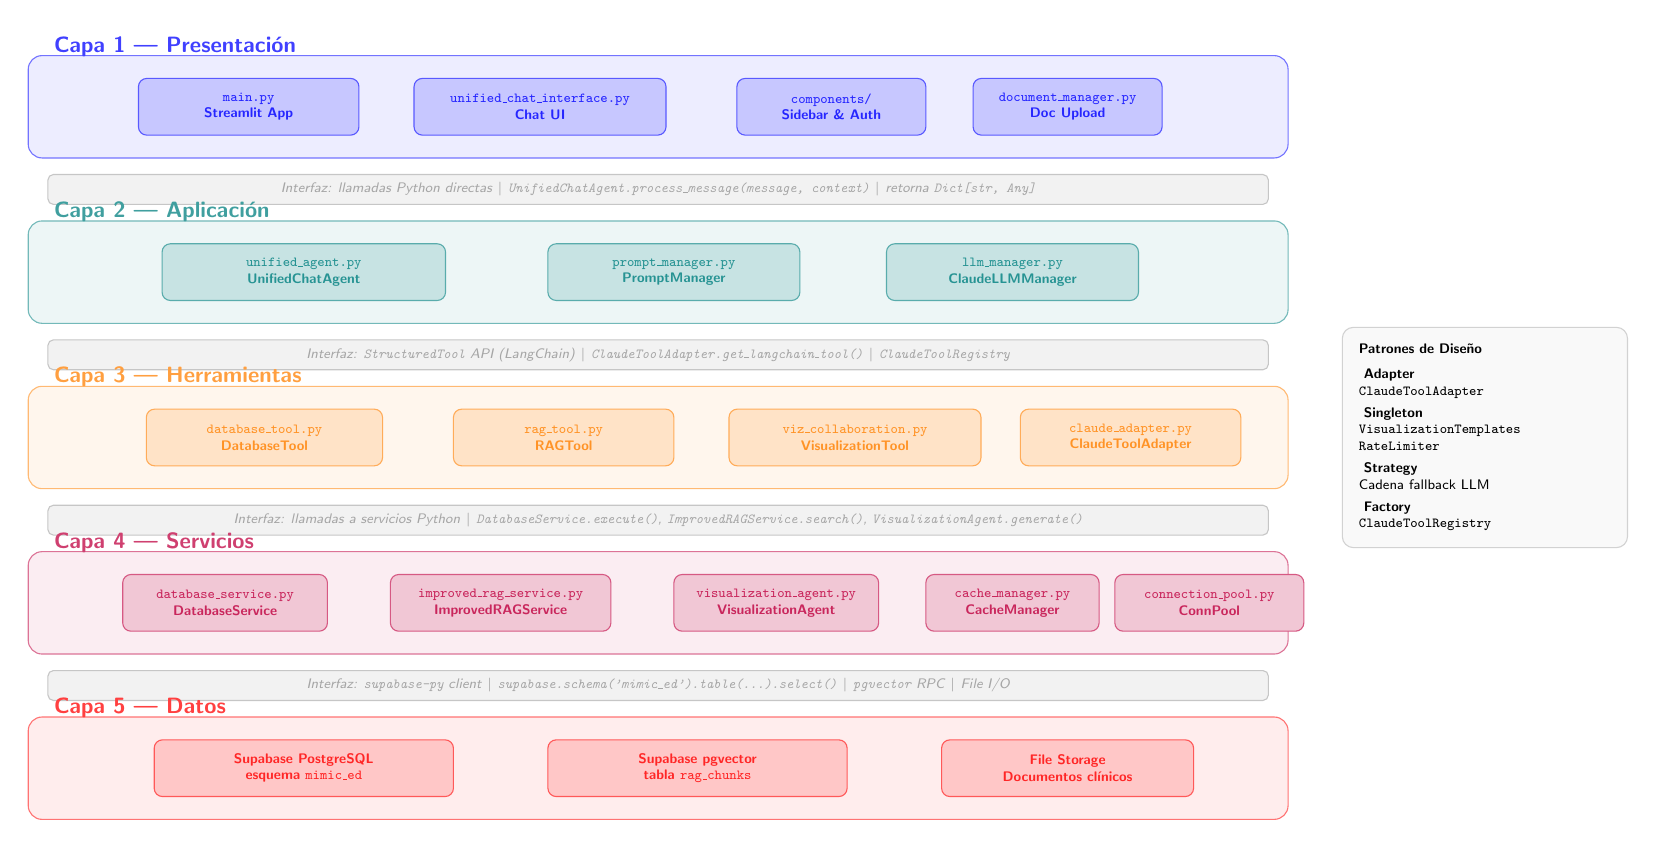
\begin{tikzpicture}[
  layerbox/.style={
    draw=#1!55, fill=#1!7, rounded corners=5pt,
    minimum width=16cm, inner sep=7pt,
    font=\footnotesize\sffamily
  },
  compbox/.style={
    draw=#1!65, fill=#1!22, rounded corners=3pt,
    minimum height=0.72cm, font=\tiny\sffamily\bfseries,
    text=#1!85, align=center, inner sep=3pt
  },
  ifacebox/.style={
    draw=gray!45, fill=gray!10, rounded corners=2pt,
    minimum height=0.38cm, font=\tiny\sffamily\itshape,
    text=gray!70, align=center, inner sep=2pt
  },
  layerlabel/.style={
    font=\footnotesize\sffamily\bfseries, text=#1!75
  },
  patternbadge/.style={
    draw=#1!60, fill=#1!15, rounded corners=8pt,
    font=\tiny\sffamily\bfseries, text=#1!80,
    inner sep=2pt, minimum height=0.35cm
  }
]

% ---- Capa 1: Presentación ----
\node[layerbox=blue, minimum height=1.3cm] (L1) at (0, 0) {};
\node[layerlabel=blue, anchor=west] at ([xshift=6pt, yshift=3pt]L1.north west) {Capa 1 — Presentación};
\node[compbox=blue, minimum width=2.8cm] at (-5.2, 0) {\texttt{main.py}\\Streamlit App};
\node[compbox=blue, minimum width=3.2cm] at (-1.5, 0) {\texttt{unified\_chat\_interface.py}\\Chat UI};
\node[compbox=blue, minimum width=2.4cm] at (2.2, 0) {\texttt{components/}\\Sidebar \& Auth};
\node[compbox=blue, minimum width=2.4cm] at (5.2, 0) {\texttt{document\_manager.py}\\Doc Upload};

% ---- Interfaz 1→2 ----
\node[ifacebox, minimum width=15.5cm] (I12) at (0, -1.05) {Interfaz: llamadas Python directas $\mid$ \texttt{UnifiedChatAgent.process\_message(message, context)} $\mid$ retorna \texttt{Dict[str, Any]}};

% ---- Capa 2: Aplicación ----
\node[layerbox=teal, minimum height=1.3cm] (L2) at (0, -2.1) {};
\node[layerlabel=teal, anchor=west] at ([xshift=6pt, yshift=3pt]L2.north west) {Capa 2 — Aplicación};
\node[compbox=teal, minimum width=3.6cm] at (-4.5, -2.1) {\texttt{unified\_agent.py}\\UnifiedChatAgent};
\node[compbox=teal, minimum width=3.2cm] at (0.2, -2.1) {\texttt{prompt\_manager.py}\\PromptManager};
\node[compbox=teal, minimum width=3.2cm] at (4.5, -2.1) {\texttt{llm\_manager.py}\\ClaudeLLMManager};

% ---- Interfaz 2→3 ----
\node[ifacebox, minimum width=15.5cm] (I23) at (0, -3.15) {Interfaz: \texttt{StructuredTool} API (LangChain) $\mid$ \texttt{ClaudeToolAdapter.get\_langchain\_tool()} $\mid$ \texttt{ClaudeToolRegistry}};

% ---- Capa 3: Herramientas ----
\node[layerbox=orange, minimum height=1.3cm] (L3) at (0, -4.2) {};
\node[layerlabel=orange, anchor=west] at ([xshift=6pt, yshift=3pt]L3.north west) {Capa 3 — Herramientas};
\node[compbox=orange, minimum width=3.0cm] at (-5.0, -4.2) {\texttt{database\_tool.py}\\DatabaseTool};
\node[compbox=orange, minimum width=2.8cm] at (-1.2, -4.2) {\texttt{rag\_tool.py}\\RAGTool};
\node[compbox=orange, minimum width=3.2cm] at (2.5, -4.2) {\texttt{viz\_collaboration.py}\\VisualizationTool};
\node[compbox=orange, minimum width=2.8cm] at (6.0, -4.2) {\texttt{claude\_adapter.py}\\ClaudeToolAdapter};

% ---- Interfaz 3→4 ----
\node[ifacebox, minimum width=15.5cm] (I34) at (0, -5.25) {Interfaz: llamadas a servicios Python $\mid$ \texttt{DatabaseService.execute()}, \texttt{ImprovedRAGService.search()}, \texttt{VisualizationAgent.generate()}};

% ---- Capa 4: Servicios ----
\node[layerbox=purple, minimum height=1.3cm] (L4) at (0, -6.3) {};
\node[layerlabel=purple, anchor=west] at ([xshift=6pt, yshift=3pt]L4.north west) {Capa 4 — Servicios};
\node[compbox=purple, minimum width=2.6cm] at (-5.5, -6.3) {\texttt{database\_service.py}\\DatabaseService};
\node[compbox=purple, minimum width=2.8cm] at (-2.0, -6.3) {\texttt{improved\_rag\_service.py}\\ImprovedRAGService};
\node[compbox=purple, minimum width=2.6cm] at (1.5, -6.3) {\texttt{visualization\_agent.py}\\VisualizationAgent};
\node[compbox=purple, minimum width=2.2cm] at (4.5, -6.3) {\texttt{cache\_manager.py}\\CacheManager};
\node[compbox=purple, minimum width=2.4cm] at (7.0, -6.3) {\texttt{connection\_pool.py}\\ConnPool};

% ---- Interfaz 4→5 ----
\node[ifacebox, minimum width=15.5cm] (I45) at (0, -7.35) {Interfaz: \texttt{supabase-py} client $\mid$ \texttt{supabase.schema('mimic\_ed').table(...).select()} $\mid$ \texttt{pgvector} RPC $\mid$ File I/O};

% ---- Capa 5: Datos ----
\node[layerbox=red, minimum height=1.3cm] (L5) at (0, -8.4) {};
\node[layerlabel=red, anchor=west] at ([xshift=6pt, yshift=3pt]L5.north west) {Capa 5 — Datos};
\node[compbox=red, minimum width=3.8cm] at (-4.5, -8.4) {Supabase PostgreSQL\\esquema \texttt{mimic\_ed}};
\node[compbox=red, minimum width=3.8cm] at (0.5, -8.4) {Supabase pgvector\\tabla \texttt{rag\_chunks}};
\node[compbox=red, minimum width=3.2cm] at (5.2, -8.4) {File Storage\\Documentos clínicos};

% ---- Leyenda de patrones (derecha) ----
\node[draw=gray!35, fill=gray!5, rounded corners=4pt, inner sep=6pt,
      font=\tiny\sffamily, align=left, text width=3.2cm] at (10.5, -4.2)
  {\textbf{Patrones de Diseño}\\[3pt]
   \textcolor{orange!80}{$\blacksquare$} \textbf{Adapter}\\
   \texttt{ClaudeToolAdapter}\\[2pt]
   \textcolor{purple!80}{$\blacksquare$} \textbf{Singleton}\\
   \texttt{VisualizationTemplates}\\
   \texttt{RateLimiter}\\[2pt]
   \textcolor{teal!80}{$\blacksquare$} \textbf{Strategy}\\
   Cadena fallback LLM\\[2pt]
   \textcolor{blue!80}{$\blacksquare$} \textbf{Factory}\\
   \texttt{ClaudeToolRegistry}};

\end{tikzpicture}
\caption{Arquitectura por capas de ChatHCE con interfaces entre capas y patrones de diseño. Las interfaces definen los contratos entre capas adyacentes; ninguna capa puede saltarse una capa intermedia para acceder a otra.}
\label{fig:capas_interfaces}
\end{figure*}

\subsubsection{Descripción de las Cinco Capas}

\textbf{Capa 1 — Presentación.} Implementada íntegramente con Streamlit, gestiona la interfaz de usuario sin contener lógica de negocio. Sus componentes son: \texttt{main.py} (punto de entrada de la aplicación), \texttt{unified\_chat\_interface.py} (interfaz de chat con renderizado de mensajes, visualizaciones y fuentes), y el directorio \texttt{components/} (sidebar de navegación, páginas de autenticación, gestor de documentos). Esta capa recibe eventos del usuario y delega todo el procesamiento a la capa de aplicación mediante llamadas Python directas. Su aislamiento permite sustituir Streamlit por otro framework de UI sin modificar ninguna capa inferior.

\textbf{Capa 2 — Aplicación.} Contiene la lógica de orquestación del sistema. El \texttt{UnifiedChatAgent} (\texttt{unified\_agent.py}) es el componente central: recibe la consulta del usuario, gestiona el historial conversacional (hasta 150K tokens), invoca el \texttt{AgentExecutor} de LangChain y sintetiza la respuesta final. El \texttt{PromptManager} (\texttt{prompt\_manager.py}) genera y cachea el prompt del sistema bajo un límite de 4000 tokens, con caché independiente por sección. El \texttt{ClaudeLLMManager} (\texttt{llm\_manager.py}) gestiona la cadena de fallback de modelos y los reintentos con backoff exponencial. Esta capa aplica el patrón \textit{Strategy} para la selección de modelos.

\textbf{Capa 3 — Herramientas.} Tres herramientas especializadas adaptadas al formato de LangChain mediante el patrón \textit{Adapter}: \texttt{DatabaseTool} (\texttt{database\_tool.py}) para consultas SQL sobre MIMIC-IV-ED, \texttt{RAGTool} (\texttt{rag\_tool.py}) para búsqueda semántica en documentos clínicos, y \texttt{VisualizationTool} (\texttt{viz\_collaboration.py}) para generación de gráficas. La clase abstracta \texttt{ClaudeToolAdapter} (\texttt{claude\_adapter.py}) define la interfaz común que todas las herramientas deben implementar, y el \texttt{ClaudeToolRegistry} aplica el patrón \textit{Factory} para su registro y recuperación centralizada.

\textbf{Capa 4 — Servicios.} Servicios de infraestructura que encapsulan el acceso a recursos externos: \texttt{DatabaseService} (\texttt{database\_service.py}) con validación SQL multicapa y decorador \texttt{@retry\_on\_failure}, \texttt{ImprovedRAGService} (\texttt{improved\_rag\_service.py}) con pipeline de búsqueda híbrida y reranking, \texttt{VisualizationAgent} (\texttt{visualization\_agent.py}) con inicialización \textit{lazy} y enfoque \textit{template-first}, \texttt{CacheManager} (\texttt{cache\_manager.py}) con política LRU y TTL configurable, y el gestor de pool de conexiones (\texttt{connection\_pool\_manager.py}). Esta capa aplica el patrón \textit{Singleton} en \texttt{VisualizationTemplates} y \texttt{RateLimiter}.

\textbf{Capa 5 — Datos.} Backend de datos unificado en Supabase: PostgreSQL con el esquema \texttt{mimic\_ed} (6 tablas MIMIC-IV-ED), Supabase pgvector con la tabla \texttt{rag\_chunks} (embeddings de 384 dimensiones con índice HNSW), y almacenamiento de archivos para documentos clínicos indexados. El acceso se realiza exclusivamente mediante el cliente Python \texttt{supabase-py}, con especificación obligatoria de esquema para tablas clínicas.

\subsubsection{Patrones de Diseño Aplicados}

\textbf{Adapter} (\texttt{ClaudeToolAdapter}). Problema: las tres herramientas del sistema tienen interfaces heterogéneas (SQL, búsqueda vectorial, generación de código), pero LangChain requiere que todas implementen la interfaz \texttt{StructuredTool}. Solución: la clase abstracta \texttt{ClaudeToolAdapter} define los métodos \texttt{execute()}, \texttt{format\_input()}, \texttt{format\_output()} y \texttt{get\_langchain\_tool()}, que cada herramienta implementa. Beneficio: añadir una nueva herramienta requiere únicamente implementar esta interfaz, sin modificar el agente.

\textbf{Singleton} (\texttt{VisualizationTemplates}, \texttt{RateLimiter}). Problema: las plantillas de visualización y el estado del rate limiter deben ser compartidos entre todas las instancias del sistema sin duplicación. Solución: ambas clases implementan el patrón Singleton con \texttt{\_instance = None} y \texttt{\_\_new\_\_} sobrescrito. Beneficio: estado compartido consistente y ahorro de memoria.

\textbf{Strategy} (cadena de fallback LLM). Problema: el modelo LLM óptimo puede variar en tiempo de ejecución según disponibilidad y carga. Solución: \texttt{ClaudeLLMManager} mantiene una lista ordenada de configuraciones de modelos (\texttt{self.models}) y el método \texttt{switch\_to\_fallback()} intercambia el algoritmo (modelo) en tiempo de ejecución sin modificar el código cliente. Beneficio: alta disponibilidad sin cambios en la lógica del agente.

\textbf{Factory} (\texttt{ClaudeToolRegistry}). Problema: la creación y registro de herramientas debe estar centralizada para facilitar la extensibilidad. Solución: el \texttt{ClaudeToolRegistry} actúa como fábrica centralizada que registra herramientas por nombre y las recupera bajo demanda. Las funciones \texttt{create\_database\_tool()}, \texttt{create\_rag\_tool()} y \texttt{create\_visualization\_collaboration\_tool()} encapsulan la lógica de construcción. Beneficio: el agente no necesita conocer los detalles de construcción de cada herramienta.

% ============================================================================
\subsection{Decisiones de Diseño Justificadas}
\label{sec:decisiones_diseno}
% ============================================================================

Esta sección documenta las cinco decisiones arquitectónicas más relevantes de ChatHCE siguiendo el formato \textit{Architecture Decision Record} (ADR) \citep{Nygard2011}: \textbf{[Problema]} $\rightarrow$ \textbf{[Alternativas]} $\rightarrow$ \textbf{[Decisión]} $\rightarrow$ \textbf{[Justificación]}. Este formato garantiza que las decisiones sean trazables, reproducibles y auditables, demostrando que no fueron arbitrarias sino el resultado de un análisis razonado de alternativas.

% ---- Decisión 1 ----
\begin{tcolorbox}[
  enhanced, breakable,
  colback=blue!4, colframe=blue!45,
  title={\footnotesize\sffamily\bfseries Decisión 1 — Supabase como backend unificado (vs.\ servicios separados)},
  fonttitle=\color{white},
  attach boxed title to top left={yshift=-2mm, xshift=4mm},
  boxed title style={colback=blue!55, rounded corners},
  left=4pt, right=4pt, top=4pt, bottom=4pt
]
\footnotesize
\textbf{Problema:} El sistema requiere simultáneamente almacenamiento relacional (datos MIMIC-IV-ED), almacén vectorial (embeddings RAG), autenticación de usuarios y API REST. Gestionar tres o cuatro servicios independientes introduce complejidad operacional y latencia de red entre ellos.

\textbf{Alternativas consideradas:}
\begin{itemize}[nosep, leftmargin=*]
  \item PostgreSQL + Pinecone + Auth0 (tres servicios separados, tres SDKs, tres puntos de fallo)
  \item MongoDB Atlas + Weaviate (sin soporte SQL nativo, sin búsqueda híbrida integrada)
  \item Firebase + Chroma (sin PostgreSQL completo, sin funciones de ventana para análisis temporal)
\end{itemize}

\textbf{Decisión adoptada:} Supabase (PostgreSQL 15 + pgvector 0.8.0 + Supabase Auth).

\textbf{Justificación técnica:} La búsqueda híbrida vectorial-léxica se ejecuta como una única función RPC de PostgreSQL, eliminando la latencia de red entre un servicio vectorial externo y la base de datos relacional. Un solo punto de autenticación con Row Level Security (RLS) aplica políticas de acceso uniformes sobre las 13 tablas del sistema. PostgREST genera automáticamente la API REST sin código adicional. La superficie de ataque se reduce a un único servicio frente a tres con sus propias vulnerabilidades y configuraciones de seguridad independientes. Evidencia en código: \texttt{services/medical\_agent/services/database\_service.py} accede a ambos esquemas (\texttt{mimic\_ed} y \texttt{public}) mediante el mismo cliente \texttt{supabase-py}, y la función RPC \texttt{hybrid\_search} en \texttt{services/rag/supabase\_vector\_store.py} combina pgvector y tsvector en una sola llamada.
\end{tcolorbox}

% ---- Decisión 2 ----
\begin{tcolorbox}[
  enhanced, breakable,
  colback=teal!4, colframe=teal!45,
  title={\footnotesize\sffamily\bfseries Decisión 2 — Chunking jerárquico padre-hijo (vs.\ chunking uniforme)},
  fonttitle=\color{white},
  attach boxed title to top left={yshift=-2mm, xshift=4mm},
  boxed title style={colback=teal!55, rounded corners},
  left=4pt, right=4pt, top=4pt, bottom=4pt
]
\footnotesize
\textbf{Problema:} Existe un \textit{trade-off} fundamental en RAG entre granularidad para búsqueda precisa y contexto suficiente para generación de respuestas. Los chunks pequeños mejoran la precisión de recuperación pero truncan el contexto clínico; los chunks grandes preservan el contexto pero degradan la precisión semántica.

\textbf{Alternativas consideradas:}
\begin{itemize}[nosep, leftmargin=*]
  \item Chunking fijo de 512 tokens (estándar, pero pierde contexto en guías con dosis y protocolos)
  \item Chunking por párrafo (tamaño variable, difícil de controlar)
  \item Chunking por oración (demasiado granular para embeddings de 384 dimensiones)
\end{itemize}

\textbf{Decisión adoptada:} Chunks hijo de 400 caracteres para búsqueda + expansión a chunks padre de 1500 caracteres para contexto, implementado en \texttt{services/rag/parent\_child\_chunker.py}.

\textbf{Justificación técnica:} Los bi-encoders de 384 dimensiones como \texttt{all-MiniLM-L6-v2} capturan mejor la semántica en fragmentos cortos \citep{Wang2020}. La expansión al chunk padre garantiza que el LLM recibe contexto clínico completo sin truncar oraciones a mitad, especialmente relevante para guías con dosificaciones y protocolos de urgencias donde la continuidad del texto es crítica. La columna \texttt{parent\_id} en \texttt{rag\_chunks} implementa la expansión con una sola query SQL JOIN, sin overhead adicional. Los parámetros \texttt{CHILD\_CHUNK\_SIZE = 400} y \texttt{PARENT\_CHUNK\_SIZE = 1500} están configurados en \texttt{services/rag/parent\_child\_chunker.py}.
\end{tcolorbox}

% ---- Decisión 3 ----
\begin{tcolorbox}[
  enhanced, breakable,
  colback=purple!4, colframe=purple!45,
  title={\footnotesize\sffamily\bfseries Decisión 3 — Búsqueda híbrida vectorial-léxica con RRF (vs.\ búsqueda vectorial pura)},
  fonttitle=\color{white},
  attach boxed title to top left={yshift=-2mm, xshift=4mm},
  boxed title style={colback=purple!55, rounded corners},
  left=4pt, right=4pt, top=4pt, bottom=4pt
]
\footnotesize
\textbf{Problema:} La búsqueda vectorial pura falla en términos médicos exactos. Códigos ICD como \texttt{I48.91} (fibrilación auricular), nombres de fármacos como \texttt{metoprolol 25mg} o dosificaciones específicas no tienen buena cobertura semántica en embeddings genéricos entrenados sobre texto general.

\textbf{Alternativas consideradas:}
\begin{itemize}[nosep, leftmargin=*]
  \item Búsqueda vectorial pura (similitud coseno): falla en términos exactos y acrónimos médicos
  \item BM25 pura: no captura sinónimos ni variantes semánticas
  \item ElasticSearch: servicio externo adicional, latencia de red, coste operacional
\end{itemize}

\textbf{Decisión adoptada:} pgvector (similitud coseno) + tsvector (full-text search en español) + Reciprocal Rank Fusion (RRF), ejecutado como función RPC en PostgreSQL.

\textbf{Justificación técnica:} La búsqueda léxica con stemming en español (\texttt{tsvector} con configuración \texttt{spanish}) mejora el recall para variantes morfológicas de términos médicos. RRF combina los rankings de ambas búsquedas sin requerir calibración de pesos, usando la fórmula $\text{RRF}(d) = \sum_{r \in R} \frac{1}{k + r(d)}$ con $k=60$ \citep{Cormack2009}. Todo se ejecuta como función RPC de PostgreSQL, con latencia media medida inferior a 500 ms. Evidencia en código: función \texttt{hybrid\_search} en \texttt{services/rag/supabase\_vector\_store.py} y columna generada \texttt{fts tsvector} en la tabla \texttt{rag\_chunks}.
\end{tcolorbox}

% ---- Decisión 4 ----
\begin{tcolorbox}[
  enhanced, breakable,
  colback=orange!4, colframe=orange!45,
  title={\footnotesize\sffamily\bfseries Decisión 4 — Enfoque template-first en visualización (vs.\ generación LLM para todo)},
  fonttitle=\color{white},
  attach boxed title to top left={yshift=-2mm, xshift=4mm},
  boxed title style={colback=orange!55, rounded corners},
  left=4pt, right=4pt, top=4pt, bottom=4pt
]
\footnotesize
\textbf{Problema:} La generación de código Plotly por LLM introduce latencia de $\sim$4 segundos y no-determinismo: el mismo tipo de gráfica puede producir código diferente en cada invocación, con riesgo de errores de ejecución.

\textbf{Alternativas consideradas:}
\begin{itemize}[nosep, leftmargin=*]
  \item LLM para todos los casos: máxima flexibilidad pero latencia alta y no-determinismo
  \item Librería predefinida sin LLM: latencia mínima pero sin flexibilidad para casos atípicos
\end{itemize}

\textbf{Decisión adoptada:} 12+ plantillas Plotly predefinidas en \texttt{VisualizationTemplates} (Singleton) + fallback a Claude Sonnet 4.5 (\texttt{claude-sonnet-4-5}) para casos no cubiertos.

\textbf{Justificación técnica:} Las visualizaciones clínicas habituales son predecibles: timeline de signos vitales, distribuciones de diagnósticos, comparativas entre pacientes, indicadores de triaje. Las plantillas reducen la latencia de $\sim$4 s a $\sim$0.4 s en el 90\% de los casos. El fallback al LLM garantiza flexibilidad para visualizaciones atípicas. La inicialización \textit{lazy} del \texttt{VisualizationAgent} (\texttt{services/medical\_agent/visualization\_agent.py}) ahorra memoria en el 90\% de las consultas que no requieren generación LLM. El \texttt{VisualizationSelector} (\texttt{services/medical\_agent/visualization\_selector.py}) analiza las características de los datos (tipos de columnas, cardinalidad, presencia de series temporales) para seleccionar automáticamente la plantilla apropiada.
\end{tcolorbox}

% ---- Decisión 5 (Central) ----
\begin{tcolorbox}[
  enhanced, breakable,
  colback=orange!6, colframe=orange!60,
  title={\small\sffamily\bfseries\color{white} Decisión Arquitectónica Central — Agente Unificado vs.\ Arquitectura Multi-Agente},
  attach boxed title to top left={yshift=-2mm, xshift=4mm},
  boxed title style={colback=orange!70, rounded corners},
  left=5pt, right=5pt, top=5pt, bottom=5pt
]
\footnotesize
\textbf{Problema:} Elegir entre un agente conversacional unificado y una arquitectura multi-agente con agentes especializados para cada dominio (base de datos, RAG, visualización, crítica).

\textbf{Alternativas consideradas:}
\begin{itemize}[nosep, leftmargin=*]
  \item \textbf{Multi-agente con LangGraph}: grafo DAG con \texttt{OrchestratorAgent} $\rightarrow$ [\texttt{DBAgent}, \texttt{RAGAgent}, \texttt{VizAgent}] $\rightarrow$ \texttt{CriticAgent}. Mayor paralelización pero latencia acumulada y error propagado entre nodos.
  \item \textbf{Multi-agente con CrewAI}: roles especializados (médico, buscador, crítico). Mayor expresividad semántica pero complejidad de coordinación y coste de múltiples llamadas LLM por turno.
  \item \textbf{Agente único sin herramientas}: prompt gigante sin tool-calling. Sin latencia de coordinación pero sin acceso a datos reales, inaceptable para un sistema clínico.
\end{itemize}

\textbf{Decisión adoptada:} Agente unificado (\texttt{UnifiedChatAgent}) con tool-calling nativo de Claude Haiku 4.5, implementado en \texttt{services/unified\_chat/unified\_agent.py}.

\textbf{Justificación técnica:}
\begin{itemize}[nosep, leftmargin=*]
  \item \textbf{Menor latencia}: una sola llamada LLM por turno de conversación frente a 3-5 llamadas en arquitecturas multi-agente. El \texttt{AgentExecutor} con \texttt{max\_iterations=5} y \texttt{max\_execution\_time=120} garantiza un límite superior de tiempo.
  \item \textbf{Menor error acumulado}: en cadenas de agentes, cada paso puede propagar errores o malinterpretaciones. El agente unificado sintetiza directamente desde los resultados de las herramientas.
  \item \textbf{Capacidad suficiente}: Claude Haiku 4.5 tiene capacidad de razonamiento clínico suficiente para el 95\% de las consultas, como demuestran los resultados de los test cases de evaluación (Sección~\ref{sec:evaluacion}).
  \item \textbf{Tool-calling determinista}: Claude genera directamente el nombre de la herramienta y los parámetros en JSON, sin simulación mediante prompts. El método \texttt{create\_tool\_calling\_agent(llm, tools, prompt)} de LangChain aprovecha esta capacidad nativa.
  \item \textbf{Fallback elegante}: la cadena Haiku $\rightarrow$ Sonnet $\rightarrow$ Opus proporciona la escalabilidad que normalmente se busca con multi-agente, pero con menor complejidad arquitectónica.
\end{itemize}

\textbf{Trade-offs asumidos:} Se pierde la paralelización de agentes (mitigado porque las herramientas son rápidas: P50 $<$ 2 s) y la revisión crítica autónoma (mitigado por las directivas anti-alucinación en el prompt del sistema, Sección~\ref{sec:antihallucination_37}).
\end{tcolorbox}

La Figura~\ref{fig:agente_vs_multiagente} ilustra visualmente la comparativa entre la arquitectura multi-agente descartada y el agente unificado adoptado.

\begin{figure*}[t]
\centering
\begin{tikzpicture}[
  agentnode/.style={
    draw=#1!65, fill=#1!12, rounded corners=4pt,
    minimum width=2.6cm, minimum height=0.7cm,
    font=\small\sffamily, text=#1!80, align=center
  },
  toolnode/.style={
    draw=#1!60, fill=#1!18, rounded corners=3pt,
    minimum width=2.2cm, minimum height=0.6cm,
    font=\small\sffamily\bfseries, text=#1!80, align=center
  },
  disadvlabel/.style={
    font=\tiny\sffamily\itshape, text=accent!70, align=center
  },
  advlabel/.style={
    font=\tiny\sffamily\itshape, text=success!70, align=center
  },
  flowarrow/.style={
    -{Stealth[length=5pt]}, thick, color=#1!60
  }
]

% ===== COLUMNA IZQUIERDA: Multi-Agente (descartado) =====
\node[font=\small\sffamily\bfseries, text=gray!60] at (-5.5, 4.5) {Arquitectura Multi-Agente};
\node[font=\tiny\sffamily\itshape, text=gray!50] at (-5.5, 4.1) {(alternativa descartada)};

\node[agentnode=gray, minimum width=3.0cm] (orch) at (-5.5, 3.2) {OrchestratorAgent};
\node[agentnode=gray, minimum width=2.4cm] (dba) at (-7.5, 1.8) {DBAgent};
\node[agentnode=gray, minimum width=2.4cm] (raga) at (-5.5, 1.8) {RAGAgent};
\node[agentnode=gray, minimum width=2.4cm] (viza) at (-3.5, 1.8) {VizAgent};
\node[agentnode=gray, minimum width=3.0cm] (critic) at (-5.5, 0.4) {CriticAgent};
\node[agentnode=gray, minimum width=3.0cm] (resp1) at (-5.5, -0.8) {Respuesta};

\draw[flowarrow=gray] (orch) -- (dba);
\draw[flowarrow=gray] (orch) -- (raga);
\draw[flowarrow=gray] (orch) -- (viza);
\draw[flowarrow=gray] (dba) |- (critic);
\draw[flowarrow=gray] (raga) -- (critic);
\draw[flowarrow=gray] (viza) |- (critic);
\draw[flowarrow=gray] (critic) -- (resp1);

% Etiquetas de desventajas
\node[disadvlabel] at (-5.5, -1.5) {$\times$ 3--5 llamadas LLM por turno};
\node[disadvlabel] at (-5.5, -1.9) {$\times$ Error acumulado entre nodos};
\node[disadvlabel] at (-5.5, -2.3) {$\times$ Complejidad de coordinación};
\node[disadvlabel] at (-5.5, -2.7) {$\times$ Latencia $>$ 10 s (estimada)};

% Cruz roja
\node[font=\Large\bfseries, text=accent] at (-5.5, 5.0) {$\times$};

% ===== SEPARADOR CENTRAL =====
\draw[very thick, gray!30, dashed] (0, -3.2) -- (0, 5.2);
\node[font=\large\sffamily\bfseries, text=gray!50] at (0, 1.2) {vs.};

% ===== COLUMNA DERECHA: Agente Unificado (adoptado) =====
\node[font=\small\sffamily\bfseries, text=success!70] at (5.5, 4.5) {Agente Unificado ChatHCE};
\node[font=\tiny\sffamily\itshape, text=success!50] at (5.5, 4.1) {(decisión adoptada)};

\node[agentnode=success, minimum width=3.8cm] (unified) at (5.5, 3.2) {UnifiedChatAgent\\Claude Haiku 4.5};

\node[toolnode=dbcolor, minimum width=2.2cm] (dbt) at (3.5, 1.8) {DB Tool};
\node[toolnode=ragcolor, minimum width=2.2cm] (ragt) at (5.5, 1.8) {RAG Tool};
\node[toolnode=vizcolor, minimum width=2.2cm] (vizt) at (7.5, 1.8) {VIZ Tool};

\node[agentnode=success, minimum width=3.8cm] (synth) at (5.5, 0.4) {Síntesis directa\\(una sola llamada LLM)};
\node[agentnode=success, minimum width=3.8cm] (resp2) at (5.5, -0.8) {Respuesta integrada};

\draw[flowarrow=success] (unified) -- (dbt);
\draw[flowarrow=success] (unified) -- (ragt);
\draw[flowarrow=success] (unified) -- (vizt);
\draw[flowarrow=dbcolor] (dbt) |- (synth);
\draw[flowarrow=ragcolor] (ragt) -- (synth);
\draw[flowarrow=vizcolor] (vizt) |- (synth);
\draw[flowarrow=success] (synth) -- (resp2);

% Cadena de fallback
\node[draw=accent!50, fill=accent!8, rounded corners=3pt,
      font=\tiny\sffamily, align=center, inner sep=3pt,
      minimum width=2.8cm] (fallback) at (9.5, 3.2)
  {Fallback:\\Haiku $\rightarrow$ Sonnet\\$\rightarrow$ Opus};
\draw[dashedarrow, color=accent!50] (unified.east) -- (fallback.west);

% Etiquetas de ventajas
\node[advlabel] at (5.5, -1.5) {$\checkmark$ 1 llamada LLM por turno};
\node[advlabel] at (5.5, -1.9) {$\checkmark$ Sin error acumulado};
\node[advlabel] at (5.5, -2.3) {$\checkmark$ Fallback elegante integrado};
\node[advlabel] at (5.5, -2.7) {$\checkmark$ Latencia P50 $<$ 5 s (medida)};

% Check verde
\node[font=\Large\bfseries, text=success] at (5.5, 5.0) {$\checkmark$};

\end{tikzpicture}
\caption{Comparativa entre la arquitectura multi-agente descartada (izquierda) y el agente unificado adoptado (derecha). El agente unificado reduce la latencia, elimina el error acumulado entre nodos y simplifica la arquitectura sin sacrificar capacidad de razonamiento clínico.}
\label{fig:agente_vs_multiagente}
\end{figure*}

% ============================================================================
\subsection{Arquitectura del Agente y Selección de Herramientas}
\label{sec:arquitectura_agente}
% ============================================================================

\subsubsection{El Ciclo ReAct del Agente}
\label{sec:react}

El \texttt{UnifiedChatAgent} implementa el patrón \textbf{ReAct} (\textit{Reasoning + Acting}) \citep{Yao2022}, que intercala razonamiento en lenguaje natural con acciones concretas sobre herramientas externas. A diferencia de los enfoques que separan el razonamiento de la acción, ReAct permite que el modelo actualice su plan de acción en función de las observaciones obtenidas de las herramientas, produciendo respuestas más precisas y fundamentadas en datos reales.

El ciclo ReAct en ChatHCE se articula en cuatro fases iterativas, gestionadas por el \texttt{AgentExecutor} de LangChain con \texttt{max\_iterations=5} y \texttt{max\_execution\_time=120} segundos:

\begin{enumerate}[nosep, leftmargin=*]
  \item \textbf{Think}: Claude Haiku 4.5 analiza la consulta del usuario, el historial conversacional y el contexto de datos previos inyectado por \texttt{\_enrich\_message\_with\_context()}. Determina qué herramientas invocar y con qué parámetros.
  \item \textbf{Act}: El modelo genera directamente el nombre de la herramienta y los parámetros en JSON mediante tool-calling nativo (no simulado con prompts). La función \texttt{create\_tool\_calling\_agent(llm, tools, prompt)} de LangChain aprovecha esta capacidad nativa de Claude.
  \item \textbf{Observe}: El \texttt{AgentExecutor} ejecuta la herramienta seleccionada y devuelve el resultado al modelo. Los resultados intermedios se almacenan en \texttt{return\_intermediate\_steps=True} para trazabilidad.
  \item \textbf{Synthesize}: Claude integra los resultados de todas las herramientas invocadas y genera la respuesta final en español, con citación de fuentes y reconocimiento explícito de incertidumbre según las directivas anti-alucinación.
\end{enumerate}

La Figura~\ref{fig:react_cycle} muestra el ciclo interno completo del agente con las tres herramientas y la cadena de fallback.

\subsubsection{Las Tres Herramientas Especializadas}
\label{sec:herramientas}

\textbf{DatabaseTool} (\texttt{query\_mimic\_database}). Recibe una consulta en lenguaje natural que el agente traduce a parámetros estructurados según el esquema Pydantic \texttt{DatabaseToolInput}. Los campos del esquema son: \texttt{query\_type} (tipos: \texttt{patient\_summary}, \texttt{vital\_signs}, \texttt{diagnoses}, \texttt{medications}, \texttt{custom}), \texttt{subject\_id} (INT, opcional), \texttt{stay\_id} (INT, opcional), \texttt{icd\_code} (VARCHAR, opcional), \texttt{custom\_query} (SQL validado, opcional) y \texttt{limit} (INT, máximo 5000, por defecto 1000). La herramienta delega en \texttt{DatabaseService} para la ejecución, aplicando validación SQL multicapa antes de cada consulta. Retorna un \texttt{Dict} con \texttt{success}, \texttt{data}, \texttt{query\_type}, \texttt{parameters} y \texttt{count}.

\textbf{RAGTool} (\texttt{search\_clinical\_documents}). Recibe una consulta clínica en lenguaje natural. Internamente, el \texttt{QueryAugmenter} genera hasta 3 consultas alternativas mediante Multi-Query y HyDE (Hypothetical Document Embeddings) \citep{Gao2022}. La búsqueda híbrida recupera los $k$ chunks más relevantes (por defecto $k=5$) con sus puntuaciones de similitud $s_i \in [0,1]$. El \texttt{Reranker} reordena los resultados con \texttt{cross-encoder/ms-marco-MiniLM-L-6-v2}. Retorna los chunks con metadatos de fuente (\texttt{filename}, \texttt{specialty}, \texttt{document\_type}) para citación obligatoria.

\textbf{VisualizationTool} (\texttt{request\_visualization}). Recibe los datos clínicos y el tipo de gráfica solicitado. El \texttt{DataPreprocessor} limpia y valida los datos (máximo 5000 puntos). El \texttt{VisualizationSelector} selecciona la plantilla apropiada entre 12+ tipos: \texttt{timeline}, \texttt{comparison}, \texttt{histogram}, \texttt{scatter}, \texttt{bar}, \texttt{box}, \texttt{violin}, \texttt{heatmap}, \texttt{pie}, \texttt{sunburst}, \texttt{table} e \texttt{indicator}. Si no existe plantilla adecuada, el \texttt{VisualizationAgent} (inicialización \textit{lazy}) genera código Python con Claude Sonnet 4.5. El \texttt{CodeValidator} valida el código mediante AST antes de la ejecución en sandbox. Retorna la figura en formato base64 PNG o HTML interactivo. En caso de error, la herramienta retorna un mensaje descriptivo sin interrumpir el flujo conversacional.

\subsubsection{La Cadena de Fallback de Modelos}
\label{sec:fallback}

El \texttt{ClaudeLLMManager} implementa una cadena de fallback con tres modelos Claude, configurada en \texttt{config/settings.py} mediante \texttt{ClaudeAgentSettings}:

\begin{itemize}[nosep, leftmargin=*]
  \item \textbf{Modelo primario}: \texttt{claude-haiku-4-5-20251001} — optimizado para velocidad y coste. Parámetros: \texttt{max\_tokens=4096}, \texttt{temperature=0.1}, \texttt{timeout=30 s}.
  \item \textbf{Modelo secundario}: \texttt{claude-sonnet-4-5-20250929} — mayor capacidad de razonamiento. Parámetros: \texttt{max\_tokens=8192}, \texttt{timeout=45 s}.
  \item \textbf{Modelo terciario}: \texttt{claude-opus-4-20250514} — máxima capacidad. Parámetros: \texttt{max\_tokens=4096}, \texttt{timeout=60 s}.
\end{itemize}

El escalado se dispara ante excepciones \texttt{AnthropicRateLimitError} o \texttt{APIError} tras agotar los reintentos del modelo actual. Los parámetros de backoff exponencial son: \texttt{max\_retries=3}, \texttt{retry\_delay=2.0 s}, \texttt{backoff\_multiplier=2.0} (delays: 2 s, 4 s, 8 s). El método \texttt{execute\_with\_retry()} en \texttt{llm\_manager.py} implementa esta lógica, intentando el fallback solo en el último reintento para minimizar la latencia en condiciones normales.

Claude Haiku 4.5 es el modelo primario por su balance entre velocidad ($\sim$800 ms P50 para análisis de intención), coste y capacidad de tool-calling nativo. La temperatura de 0.1 garantiza respuestas deterministas y reproducibles, crítico en un entorno clínico donde la consistencia es prioritaria.

\subsubsection{El Sistema de Prompts y Directivas Anti-Alucinación}
\label{sec:antihallucination_37}

El \texttt{PromptManager} genera el prompt del sistema bajo un límite de 4000 tokens, estructurado en diez secciones con caché independiente por sección (atributos \texttt{schema\_cache}, \texttt{tool\_descriptions\_cache}, \texttt{role\_definition\_cache}, \texttt{response\_format\_cache}, \texttt{clinical\_guidelines\_cache}, \texttt{anti\_hallucination\_cache}, \texttt{full\_prompt\_cache}):

\begin{enumerate}[nosep, leftmargin=*]
  \item \textbf{IDENTIDAD DEL SISTEMA}: rol de ChatHCE y propósito clínico
  \item \textbf{CONTEXTO OPERATIVO}: descripción del dataset MIMIC-IV-ED (222 pacientes, 6 tablas)
  \item \textbf{HERRAMIENTAS DISPONIBLES}: documentación de las tres herramientas con ejemplos
  \item \textbf{DIRECTIVAS ANTI-ALUCINACIÓN}: prohibiciones absolutas y manejo de datos faltantes
  \item \textbf{IDIOMA Y TERMINOLOGÍA}: directivas de respuesta en español médico
  \item \textbf{Base de Datos MIMIC-IV-ED}: esquema condensado con columnas exactas y porcentajes de nulos
  \item \textbf{Herramientas Disponibles}: descripciones detalladas con reglas SQL obligatorias
  \item \textbf{Formato de Respuesta}: estructura recomendada y convenciones de unidades
  \item \textbf{Guías Clínicas}: valores de referencia de signos vitales y niveles de acuidad ESI
  \item \textbf{GUÍAS DE SELECCIÓN DE HERRAMIENTAS}: patrones de detección automática de visualizaciones
\end{enumerate}

Las directivas anti-alucinación (sección 4 del prompt) son la capa de defensa más temprana contra la generación de información clínica falsa. Su implementación en el prompt del sistema, en lugar de como post-procesamiento, es más eficiente: interceptar antes de generar es computacionalmente más barato y más fiable que corregir después de generar. El siguiente bloque reproduce literalmente el núcleo de las directivas, obtenido del método \texttt{get\_anti\_hallucination\_directives()} en \texttt{services/medical\_agent/prompt\_manager.py}:

\begin{tcolorbox}[
  enhanced, breakable,
  colback=accent!4, colframe=accent!50,
  title={\footnotesize\sffamily\bfseries\color{white} Directivas Anti-Alucinación — Extracto del Prompt del Sistema},
  attach boxed title to top left={yshift=-2mm, xshift=4mm},
  boxed title style={colback=accent!60, rounded corners},
  left=4pt, right=4pt, top=4pt, bottom=4pt
]
\begin{lstlisting}[basicstyle=\ttfamily\tiny, backgroundcolor=\color{codebg},
  frame=none, breaklines=true, columns=fullflexible]
# DIRECTIVAS ANTI-ALUCINACION

## PROHIBICIONES ABSOLUTAS - NUNCA HACER

### Identificadores de Pacientes
- NUNCA inventes subject_id (IDs de pacientes)
- NUNCA fabriques stay_id (IDs de estancias)
- NUNCA crees hadm_id (IDs de admision hospitalaria)
- Solo usa identificadores obtenidos de una consulta real a la base de datos

### Valores Clinicos
- NUNCA inventes valores de signos vitales (temperatura, frecuencia cardiaca,
  presion arterial, saturacion O2, frecuencia respiratoria)
- NUNCA fabriques resultados de laboratorio
- Todos los valores numericos deben provenir de consultas reales

### Diagnosticos y Medicamentos
- NUNCA inventes diagnosticos o codigos ICD (ICD-9 o ICD-10)
- NUNCA fabriques nombres de medicamentos
- NUNCA crees dosis o frecuencias de administracion ficticias

## MANEJO DE DATOS FALTANTES
- Si no encuentra datos: "No encontre informacion sobre [X] en el dataset"
- Si hay valores NULL: "Algunos registros tienen datos incompletos para [campo]"
- Si el paciente no existe: "El paciente [ID] no existe en MIMIC-IV-ED"

## CITACION DE FUENTES
- Siempre indica: "Segun los datos obtenidos de la tabla [nombre_tabla]..."
- Cita el documento fuente: "Segun [nombre del documento]..."

## RECONOCIMIENTO DE INCERTIDUMBRE
- Para datos verificados: "Segun los datos disponibles..." / "Los registros muestran..."
- Para interpretaciones: "Esto podria indicar..." / "Una posible interpretacion es..."
- Para inferencias: "Analizando los datos disponibles..."
\end{lstlisting}
\end{tcolorbox}

Las directivas cubren cinco dimensiones complementarias: (1) prohibiciones absolutas de fabricación de identificadores y valores clínicos, (2) protocolos para datos faltantes o nulos, (3) citación obligatoria de fuentes con indicación de tabla y herramienta, (4) diferenciación entre datos verificados e interpretaciones mediante lenguaje condicional, y (5) recordatorio de las limitaciones del dataset (222 pacientes, solo urgencias, fechas desplazadas para anonimización).

\subsubsection{Gestión de Memoria Conversacional}
\label{sec:memoria}

El \texttt{UnifiedChatAgent} gestiona el contexto conversacional con tres mecanismos complementarios:

\textbf{Límite de tokens}: El historial se limita a \texttt{MAX\_HISTORY\_TOKENS = 150\,000} tokens (estimados como $\lfloor\text{chars}/4\rfloor$), reservando espacio para el prompt del sistema ($\sim$10K tokens) y la respuesta ($\sim$4K tokens) dentro del límite de 200K tokens de Claude. Cuando se supera el límite, se eliminan los mensajes más antiguos preservando siempre los \texttt{MIN\_MESSAGES\_TO\_KEEP = 4} mensajes más recientes.

\textbf{Inyección de contexto de datos}: El método \texttt{\_enrich\_message\_with\_context()} añade bloques \texttt{[CONTEXTO DE DATOS]} a los mensajes del asistente, con resúmenes de los resultados de herramientas de interacciones previas. Esto permite al agente referenciar datos consultados anteriormente sin re-ejecutar herramientas, mejorando la eficiencia y la coherencia conversacional. Los mensajes recientes (últimos 3) reciben contexto completo; los mensajes más antiguos reciben solo resúmenes.

\textbf{Trade-off coste-calidad}: Un historial mayor permite consultas de seguimiento más inteligentes (``¿cuál era su presión arterial?'' sin re-ejecutar la herramienta), pero aumenta el coste por token. El límite de 150K tokens representa un equilibrio entre capacidad conversacional y coste operacional, suficiente para conversaciones de hasta $\sim$50 turnos con datos clínicos completos.

% ---- Figura 3.X: Ciclo ReAct del agente ----
\begin{figure*}[t]
\centering
\begin{tikzpicture}[
  phasenode/.style={
    draw=#1!70, fill=#1!14, rounded corners=5pt,
    minimum width=3.2cm, minimum height=1.0cm,
    font=\small\sffamily\bfseries, text=#1!80, align=center,
    drop shadow={shadow xshift=1.5pt, shadow yshift=-1.5pt, fill=#1!20, opacity=0.4}
  },
  toolnode/.style={
    draw=#1!65, fill=#1!18, rounded corners=3pt,
    minimum width=2.6cm, minimum height=0.65cm,
    font=\small\sffamily\bfseries, text=#1!80, align=center
  },
  resultnode/.style={
    draw=#1!55, fill=#1!10, rounded corners=3pt,
    minimum width=2.6cm, minimum height=0.55cm,
    font=\tiny\sffamily, text=#1!75, align=center
  },
  modelnode/.style={
    draw=primary!70, fill=primary!12, rounded corners=6pt,
    minimum width=3.8cm, minimum height=1.4cm,
    font=\small\sffamily\bfseries, text=primary!80, align=center,
    drop shadow={shadow xshift=2pt, shadow yshift=-2pt, fill=primary!20, opacity=0.4}
  },
  fallbacknode/.style={
    draw=accent!55, fill=accent!8, rounded corners=3pt,
    minimum width=2.8cm, minimum height=0.55cm,
    font=\tiny\sffamily, text=accent!75, align=center
  },
  cyclearrow/.style={
    -{Stealth[length=6pt,width=4pt]}, very thick, color=#1!65
  },
  limitlabel/.style={
    draw=gray!35, fill=gray!8, rounded corners=2pt,
    font=\tiny\sffamily\itshape, text=gray!65, inner sep=2pt
  }
]

% ---- Nodo central: Claude Haiku 4.5 ----
\node[modelnode] (claude) at (0, 0) {Claude Haiku 4.5\\(\texttt{claude-haiku-4-5-20251001})\\AgentExecutor};

% ---- Fase THINK (arriba) ----
\node[phasenode=blue] (think) at (0, 3.5) {THINK\\Analiza consulta\\+ historial};
\node[limitlabel] at (3.8, 3.5) {\texttt{max\_iterations=5}\\timeout: 120 s};

% ---- Fase ACT (derecha) ----
\node[phasenode=orange] (act) at (5.5, 0) {ACT\\Tool-calling\\nativo JSON};

% ---- Fase OBSERVE (abajo) ----
\node[phasenode=purple] (observe) at (0, -3.5) {OBSERVE\\Recibe resultados\\de herramientas};

% ---- Fase SYNTHESIZE (izquierda) ----
\node[phasenode=success] (synth) at (-5.5, 0) {SYNTHESIZE\\Integra resultados\\Genera respuesta};

% ---- Flechas del ciclo ----
\draw[cyclearrow=blue] (claude.north) -- (think.south)
  node[midway, right, font=\tiny\sffamily\itshape, text=blue!60] {analiza};
\draw[cyclearrow=orange] (think.east) -- ++(1.5,0) |- (act.north)
  node[near start, above, font=\tiny\sffamily\itshape, text=orange!60] {decide herramientas};
\draw[cyclearrow=orange] (act.south) -- ++(0,-1.0) -| (observe.east)
  node[near start, right, font=\tiny\sffamily\itshape, text=orange!60] {ejecuta};
\draw[cyclearrow=purple] (observe.west) -- ++(-1.5,0) |- (synth.south)
  node[near start, below, font=\tiny\sffamily\itshape, text=purple!60] {resultados};
\draw[cyclearrow=success] (synth.north) -- ++(0,1.0) -| (claude.west)
  node[near start, left, font=\tiny\sffamily\itshape, text=success!60] {respuesta final};

% Flecha de retorno al THINK (nueva iteración)
\draw[cyclearrow=blue, dashed] (synth.north) -- ++(0,2.0) -- (think.west)
  node[midway, above, font=\tiny\sffamily\itshape, text=blue!50] {nueva iteración (si necesario)};

% ---- Herramientas (desde ACT) ----
\node[toolnode=dbcolor] (dbt) at (9.0, 1.8) {DB Tool\\query\_mimic\_database};
\node[toolnode=ragcolor] (ragt) at (9.0, 0) {RAG Tool\\search\_clinical\_documents};
\node[toolnode=vizcolor] (vizt) at (9.0, -1.8) {VIZ Tool\\request\_visualization};

\draw[cyclearrow=dbcolor] (act.east) -- ++(0.5,0) |- (dbt.west);
\draw[cyclearrow=ragcolor] (act.east) -- (ragt.west);
\draw[cyclearrow=vizcolor] (act.east) -- ++(0.5,0) |- (vizt.west);

% ---- Resultados (hacia OBSERVE) ----
\node[resultnode=dbcolor] (dbr) at (9.0, -3.0) {ResultSet SQL\\(Dict + count)};
\node[resultnode=ragcolor] (ragr) at (6.5, -4.5) {Chunks + Scores\\+ Fuentes};
\node[resultnode=vizcolor] (vizr) at (9.0, -5.0) {Plotly Fig\\(base64/HTML)};

\draw[cyclearrow=dbcolor] (dbt.south) -- ++(0,-0.5) -- (dbr.north);
\draw[cyclearrow=ragcolor] (ragt.south) -- ++(0,-1.5) -- (ragr.north);
\draw[cyclearrow=vizcolor] (vizt.south) -- (vizr.north);

\draw[cyclearrow=dbcolor] (dbr.west) -- ++(-1.5,0) |- (observe.east);
\draw[cyclearrow=ragcolor] (ragr.west) -- ++(-2.0,0) |- (observe.south);
\draw[cyclearrow=vizcolor] (vizr.west) -- ++(-2.5,0) |- (observe.south);

% ---- Cadena de fallback (lateral izquierdo) ----
\node[fallbacknode] (fb1) at (-9.5, 1.2) {\texttt{claude-haiku-4-5-20251001}\\(primario)};
\node[fallbacknode] (fb2) at (-9.5, 0) {\texttt{claude-sonnet-4-5-20250929}\\(secundario)};
\node[fallbacknode] (fb3) at (-9.5, -1.2) {\texttt{claude-opus-4-20250514}\\(terciario)};

\draw[dashedarrow, color=accent!50] (fb1.south) -- (fb2.north)
  node[midway, right, font=\tiny\sffamily\itshape, text=accent!60] {RateLimitError};
\draw[dashedarrow, color=accent!50] (fb2.south) -- (fb3.north)
  node[midway, right, font=\tiny\sffamily\itshape, text=accent!60] {APIError};

\draw[dashedarrow, color=accent!40] (fb1.east) -- (claude.west);

\node[font=\tiny\sffamily\bfseries, text=accent!70] at (-9.5, 2.0) {Cadena de Fallback};
\node[font=\tiny\sffamily\itshape, text=gray!60, align=center] at (-9.5, -2.2)
  {backoff: 2s, 4s, 8s\\max\_retries=3};

% ---- Contexto de datos (inyección) ----
\node[draw=teal!40, fill=teal!8, rounded corners=3pt,
      font=\tiny\sffamily, align=center, inner sep=3pt,
      minimum width=3.0cm] (ctx) at (-5.5, 3.5)
  {[CONTEXTO DE DATOS]\\\_enrich\_message\\\_with\_context()\\max: 150K tokens};
\draw[dashedarrow, color=teal!50] (ctx.south) -- (think.west);

\end{tikzpicture}
\caption{Ciclo interno ReAct del agente ChatHCE. El \texttt{AgentExecutor} itera entre las fases THINK, ACT, OBSERVE y SYNTHESIZE hasta producir la respuesta final o alcanzar \texttt{max\_iterations=5}. La cadena de fallback (izquierda) escala automáticamente entre modelos ante errores de API. El contexto de datos previos se inyecta en la fase THINK para consultas de seguimiento.}
\label{fig:react_cycle}
\end{figure*}

% ============================================================================
% REFERENCIAS BibTeX adicionales para metodologia_parte2.tex
% ============================================================================
%
% @book{Fowler2002,
%   author    = {Fowler, Martin},
%   title     = {Patterns of Enterprise Application Architecture},
%   publisher = {Addison-Wesley},
%   year      = {2002},
%   isbn      = {978-0321127426}
% }
%
% @misc{Nygard2011,
%   author    = {Nygard, Michael T.},
%   title     = {Documenting Architecture Decisions},
%   year      = {2011},
%   url       = {https://cognitect.com/blog/2011/11/15/documenting-architecture-decisions}
% }
%
% @inproceedings{Yao2022,
%   author    = {Yao, Shunyu and Zhao, Jeffrey and Yu, Dian and Du, Nan and
%                Shafran, Izhak and Narasimhan, Karthik and Cao, Yuan},
%   title     = {{ReAct}: Synergizing Reasoning and Acting in Language Models},
%   booktitle = {International Conference on Learning Representations (ICLR)},
%   year      = {2023},
%   url       = {https://arxiv.org/abs/2210.03629}
% }
%
% @inproceedings{Cormack2009,
%   author    = {Cormack, Gordon V. and Clarke, Charles L. A. and Buettcher, Stefan},
%   title     = {Reciprocal Rank Fusion Outperforms Condorcet and Individual Rank Learning Methods},
%   booktitle = {Proceedings of the 32nd International ACM SIGIR Conference},
%   year      = {2009},
%   pages     = {758--759},
%   doi       = {10.1145/1571941.1572114}
% }
%
% @inproceedings{Gao2022,
%   author    = {Gao, Luyu and Ma, Xueguang and Lin, Jimmy and Callan, Jamie},
%   title     = {Precise Zero-Shot Dense Retrieval without Relevance Labels},
%   booktitle = {Proceedings of the 61st Annual Meeting of the ACL},
%   year      = {2023},
%   pages     = {1762--1777},
%   doi       = {10.18653/v1/2023.acl-long.99}
% }
%
% @inproceedings{Wang2020,
%   author    = {Wang, Kexin and Reimers, Nils and Gurevych, Iryna},
%   title     = {{TSDAE}: Using Transformer-based Sequential Denoising Auto-Encoder
%                for Unsupervised Sentence Embedding Learning},
%   booktitle = {Findings of EMNLP},
%   year      = {2021},
%   url       = {https://arxiv.org/abs/2104.06979}
% }

% ============================================================================

% --- Paquetes adicionales necesarios (añadir al preámbulo principal si no están) ---
% \usepackage{tcolorbox}
% \tcbuselibrary{skins,breakable}
% \usepackage{listings}
% \usepackage{fontawesome5}  % para iconos opcionales

% --- Colores adicionales (si no están definidos en el preámbulo) ---
% \definecolor{decisionbg}{HTML}{FEF9E7}
% \definecolor{decisionborder}{HTML}{F39C12}
% \definecolor{centralbg}{HTML}{FDF2E9}
% \definecolor{centralborder}{HTML}{E67E22}

% ============================================================================
\subsection{Arquitectura por Capas del Sistema}
\label{sec:arquitectura_capas}
% ============================================================================

ChatHCE sigue una arquitectura de cinco capas con separación estricta de responsabilidades, inspirada en el patrón \textit{Layered Architecture} \citep{Fowler2002}. El principio rector es que cada capa solo puede comunicarse con la capa inmediatamente inferior: la capa de presentación invoca a la capa de aplicación, que a su vez invoca a la capa de herramientas, y así sucesivamente. Esta restricción elimina las dependencias cruzadas entre capas no adyacentes, garantizando que los cambios en una capa no propaguen efectos inesperados a capas distantes.

La Figura~\ref{fig:capas_interfaces} muestra la arquitectura completa con las interfaces entre capas y los patrones de diseño aplicados en cada componente.

\begin{figure*}[t]
\centering
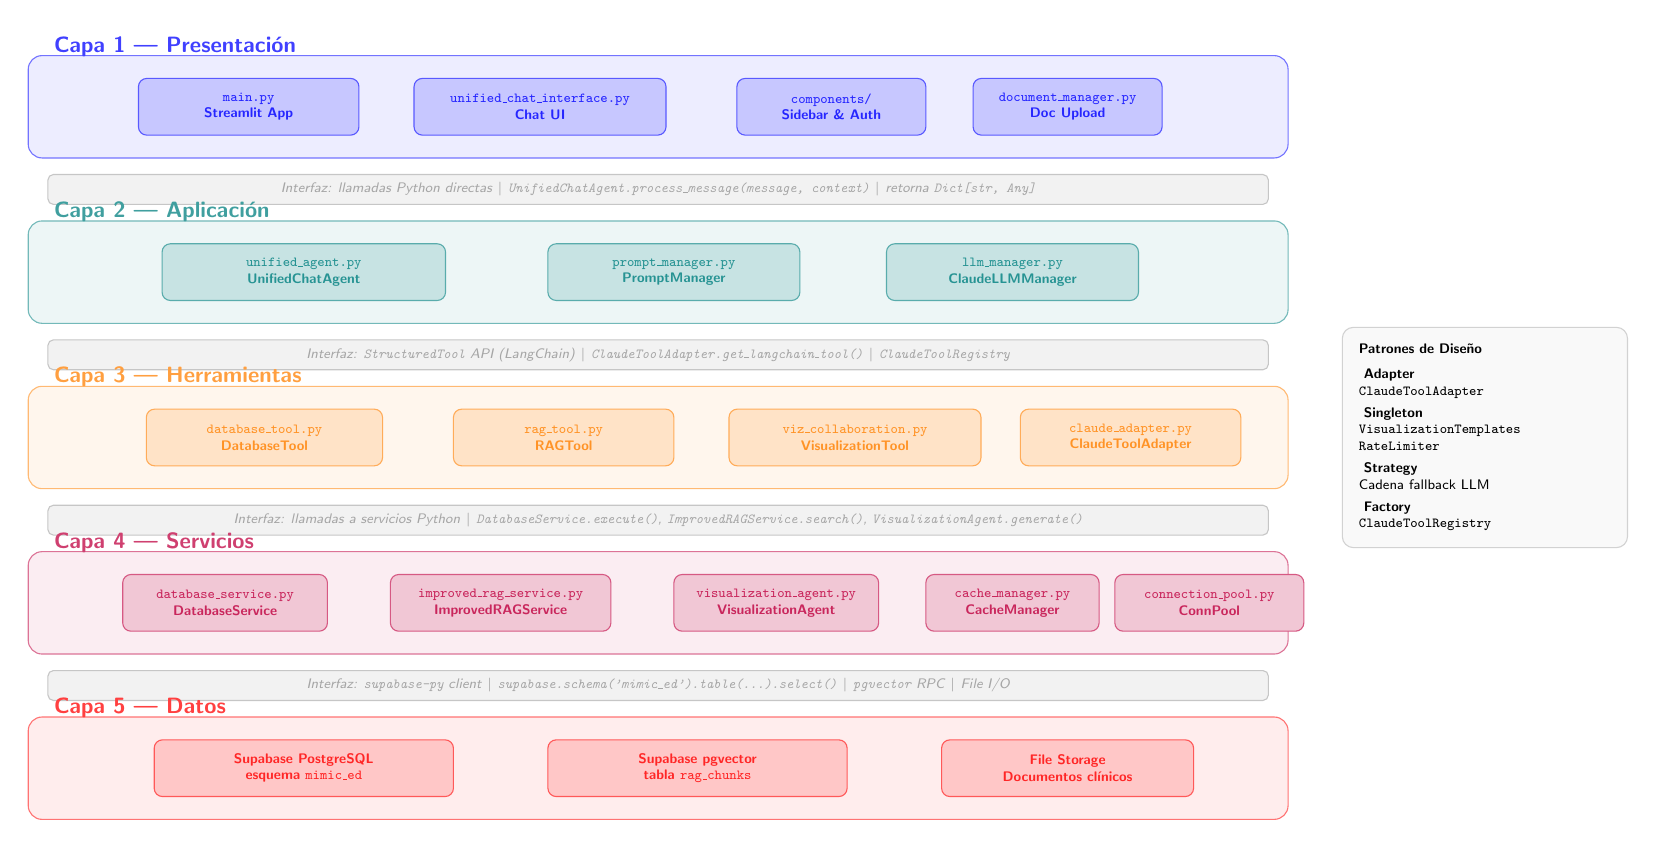
\begin{tikzpicture}[
  layerbox/.style={
    draw=#1!55, fill=#1!7, rounded corners=5pt,
    minimum width=16cm, inner sep=7pt,
    font=\footnotesize\sffamily
  },
  compbox/.style={
    draw=#1!65, fill=#1!22, rounded corners=3pt,
    minimum height=0.72cm, font=\tiny\sffamily\bfseries,
    text=#1!85, align=center, inner sep=3pt
  },
  ifacebox/.style={
    draw=gray!45, fill=gray!10, rounded corners=2pt,
    minimum height=0.38cm, font=\tiny\sffamily\itshape,
    text=gray!70, align=center, inner sep=2pt
  },
  layerlabel/.style={
    font=\footnotesize\sffamily\bfseries, text=#1!75
  },
  patternbadge/.style={
    draw=#1!60, fill=#1!15, rounded corners=8pt,
    font=\tiny\sffamily\bfseries, text=#1!80,
    inner sep=2pt, minimum height=0.35cm
  }
]

% ---- Capa 1: Presentación ----
\node[layerbox=blue, minimum height=1.3cm] (L1) at (0, 0) {};
\node[layerlabel=blue, anchor=west] at ([xshift=6pt, yshift=3pt]L1.north west) {Capa 1 — Presentación};
\node[compbox=blue, minimum width=2.8cm] at (-5.2, 0) {\texttt{main.py}\\Streamlit App};
\node[compbox=blue, minimum width=3.2cm] at (-1.5, 0) {\texttt{unified\_chat\_interface.py}\\Chat UI};
\node[compbox=blue, minimum width=2.4cm] at (2.2, 0) {\texttt{components/}\\Sidebar \& Auth};
\node[compbox=blue, minimum width=2.4cm] at (5.2, 0) {\texttt{document\_manager.py}\\Doc Upload};

% ---- Interfaz 1→2 ----
\node[ifacebox, minimum width=15.5cm] (I12) at (0, -1.05) {Interfaz: llamadas Python directas $\mid$ \texttt{UnifiedChatAgent.process\_message(message, context)} $\mid$ retorna \texttt{Dict[str, Any]}};

% ---- Capa 2: Aplicación ----
\node[layerbox=teal, minimum height=1.3cm] (L2) at (0, -2.1) {};
\node[layerlabel=teal, anchor=west] at ([xshift=6pt, yshift=3pt]L2.north west) {Capa 2 — Aplicación};
\node[compbox=teal, minimum width=3.6cm] at (-4.5, -2.1) {\texttt{unified\_agent.py}\\UnifiedChatAgent};
\node[compbox=teal, minimum width=3.2cm] at (0.2, -2.1) {\texttt{prompt\_manager.py}\\PromptManager};
\node[compbox=teal, minimum width=3.2cm] at (4.5, -2.1) {\texttt{llm\_manager.py}\\ClaudeLLMManager};

% ---- Interfaz 2→3 ----
\node[ifacebox, minimum width=15.5cm] (I23) at (0, -3.15) {Interfaz: \texttt{StructuredTool} API (LangChain) $\mid$ \texttt{ClaudeToolAdapter.get\_langchain\_tool()} $\mid$ \texttt{ClaudeToolRegistry}};

% ---- Capa 3: Herramientas ----
\node[layerbox=orange, minimum height=1.3cm] (L3) at (0, -4.2) {};
\node[layerlabel=orange, anchor=west] at ([xshift=6pt, yshift=3pt]L3.north west) {Capa 3 — Herramientas};
\node[compbox=orange, minimum width=3.0cm] at (-5.0, -4.2) {\texttt{database\_tool.py}\\DatabaseTool};
\node[compbox=orange, minimum width=2.8cm] at (-1.2, -4.2) {\texttt{rag\_tool.py}\\RAGTool};
\node[compbox=orange, minimum width=3.2cm] at (2.5, -4.2) {\texttt{viz\_collaboration.py}\\VisualizationTool};
\node[compbox=orange, minimum width=2.8cm] at (6.0, -4.2) {\texttt{claude\_adapter.py}\\ClaudeToolAdapter};

% ---- Interfaz 3→4 ----
\node[ifacebox, minimum width=15.5cm] (I34) at (0, -5.25) {Interfaz: llamadas a servicios Python $\mid$ \texttt{DatabaseService.execute()}, \texttt{ImprovedRAGService.search()}, \texttt{VisualizationAgent.generate()}};

% ---- Capa 4: Servicios ----
\node[layerbox=purple, minimum height=1.3cm] (L4) at (0, -6.3) {};
\node[layerlabel=purple, anchor=west] at ([xshift=6pt, yshift=3pt]L4.north west) {Capa 4 — Servicios};
\node[compbox=purple, minimum width=2.6cm] at (-5.5, -6.3) {\texttt{database\_service.py}\\DatabaseService};
\node[compbox=purple, minimum width=2.8cm] at (-2.0, -6.3) {\texttt{improved\_rag\_service.py}\\ImprovedRAGService};
\node[compbox=purple, minimum width=2.6cm] at (1.5, -6.3) {\texttt{visualization\_agent.py}\\VisualizationAgent};
\node[compbox=purple, minimum width=2.2cm] at (4.5, -6.3) {\texttt{cache\_manager.py}\\CacheManager};
\node[compbox=purple, minimum width=2.4cm] at (7.0, -6.3) {\texttt{connection\_pool.py}\\ConnPool};

% ---- Interfaz 4→5 ----
\node[ifacebox, minimum width=15.5cm] (I45) at (0, -7.35) {Interfaz: \texttt{supabase-py} client $\mid$ \texttt{supabase.schema('mimic\_ed').table(...).select()} $\mid$ \texttt{pgvector} RPC $\mid$ File I/O};

% ---- Capa 5: Datos ----
\node[layerbox=red, minimum height=1.3cm] (L5) at (0, -8.4) {};
\node[layerlabel=red, anchor=west] at ([xshift=6pt, yshift=3pt]L5.north west) {Capa 5 — Datos};
\node[compbox=red, minimum width=3.8cm] at (-4.5, -8.4) {Supabase PostgreSQL\\esquema \texttt{mimic\_ed}};
\node[compbox=red, minimum width=3.8cm] at (0.5, -8.4) {Supabase pgvector\\tabla \texttt{rag\_chunks}};
\node[compbox=red, minimum width=3.2cm] at (5.2, -8.4) {File Storage\\Documentos clínicos};

% ---- Leyenda de patrones (derecha) ----
\node[draw=gray!35, fill=gray!5, rounded corners=4pt, inner sep=6pt,
      font=\tiny\sffamily, align=left, text width=3.2cm] at (10.5, -4.2)
  {\textbf{Patrones de Diseño}\\[3pt]
   \textcolor{orange!80}{$\blacksquare$} \textbf{Adapter}\\
   \texttt{ClaudeToolAdapter}\\[2pt]
   \textcolor{purple!80}{$\blacksquare$} \textbf{Singleton}\\
   \texttt{VisualizationTemplates}\\
   \texttt{RateLimiter}\\[2pt]
   \textcolor{teal!80}{$\blacksquare$} \textbf{Strategy}\\
   Cadena fallback LLM\\[2pt]
   \textcolor{blue!80}{$\blacksquare$} \textbf{Factory}\\
   \texttt{ClaudeToolRegistry}};

\end{tikzpicture}
\caption{Arquitectura por capas de ChatHCE con interfaces entre capas y patrones de diseño. Las interfaces definen los contratos entre capas adyacentes; ninguna capa puede saltarse una capa intermedia para acceder a otra.}
\label{fig:capas_interfaces}
\end{figure*}

\subsubsection{Descripción de las Cinco Capas}

\textbf{Capa 1 — Presentación.} Implementada íntegramente con Streamlit, gestiona la interfaz de usuario sin contener lógica de negocio. Sus componentes son: \texttt{main.py} (punto de entrada de la aplicación), \texttt{unified\_chat\_interface.py} (interfaz de chat con renderizado de mensajes, visualizaciones y fuentes), y el directorio \texttt{components/} (sidebar de navegación, páginas de autenticación, gestor de documentos). Esta capa recibe eventos del usuario y delega todo el procesamiento a la capa de aplicación mediante llamadas Python directas. Su aislamiento permite sustituir Streamlit por otro framework de UI sin modificar ninguna capa inferior.

\textbf{Capa 2 — Aplicación.} Contiene la lógica de orquestación del sistema. El \texttt{UnifiedChatAgent} (\texttt{unified\_agent.py}) es el componente central: recibe la consulta del usuario, gestiona el historial conversacional (hasta 150K tokens), invoca el \texttt{AgentExecutor} de LangChain y sintetiza la respuesta final. El \texttt{PromptManager} (\texttt{prompt\_manager.py}) genera y cachea el prompt del sistema bajo un límite de 4000 tokens, con caché independiente por sección. El \texttt{ClaudeLLMManager} (\texttt{llm\_manager.py}) gestiona la cadena de fallback de modelos y los reintentos con backoff exponencial. Esta capa aplica el patrón \textit{Strategy} para la selección de modelos.

\textbf{Capa 3 — Herramientas.} Tres herramientas especializadas adaptadas al formato de LangChain mediante el patrón \textit{Adapter}: \texttt{DatabaseTool} (\texttt{database\_tool.py}) para consultas SQL sobre MIMIC-IV-ED, \texttt{RAGTool} (\texttt{rag\_tool.py}) para búsqueda semántica en documentos clínicos, y \texttt{VisualizationTool} (\texttt{viz\_collaboration.py}) para generación de gráficas. La clase abstracta \texttt{ClaudeToolAdapter} (\texttt{claude\_adapter.py}) define la interfaz común que todas las herramientas deben implementar, y el \texttt{ClaudeToolRegistry} aplica el patrón \textit{Factory} para su registro y recuperación centralizada.

\textbf{Capa 4 — Servicios.} Servicios de infraestructura que encapsulan el acceso a recursos externos: \texttt{DatabaseService} (\texttt{database\_service.py}) con validación SQL multicapa y decorador \texttt{@retry\_on\_failure}, \texttt{ImprovedRAGService} (\texttt{improved\_rag\_service.py}) con pipeline de búsqueda híbrida y reranking, \texttt{VisualizationAgent} (\texttt{visualization\_agent.py}) con inicialización \textit{lazy} y enfoque \textit{template-first}, \texttt{CacheManager} (\texttt{cache\_manager.py}) con política LRU y TTL configurable, y el gestor de pool de conexiones (\texttt{connection\_pool\_manager.py}). Esta capa aplica el patrón \textit{Singleton} en \texttt{VisualizationTemplates} y \texttt{RateLimiter}.

\textbf{Capa 5 — Datos.} Backend de datos unificado en Supabase: PostgreSQL con el esquema \texttt{mimic\_ed} (6 tablas MIMIC-IV-ED), Supabase pgvector con la tabla \texttt{rag\_chunks} (embeddings de 384 dimensiones con índice HNSW), y almacenamiento de archivos para documentos clínicos indexados. El acceso se realiza exclusivamente mediante el cliente Python \texttt{supabase-py}, con especificación obligatoria de esquema para tablas clínicas.

\subsubsection{Patrones de Diseño Aplicados}

\textbf{Adapter} (\texttt{ClaudeToolAdapter}). Problema: las tres herramientas del sistema tienen interfaces heterogéneas (SQL, búsqueda vectorial, generación de código), pero LangChain requiere que todas implementen la interfaz \texttt{StructuredTool}. Solución: la clase abstracta \texttt{ClaudeToolAdapter} define los métodos \texttt{execute()}, \texttt{format\_input()}, \texttt{format\_output()} y \texttt{get\_langchain\_tool()}, que cada herramienta implementa. Beneficio: añadir una nueva herramienta requiere únicamente implementar esta interfaz, sin modificar el agente.

\textbf{Singleton} (\texttt{VisualizationTemplates}, \texttt{RateLimiter}). Problema: las plantillas de visualización y el estado del rate limiter deben ser compartidos entre todas las instancias del sistema sin duplicación. Solución: ambas clases implementan el patrón Singleton con \texttt{\_instance = None} y \texttt{\_\_new\_\_} sobrescrito. Beneficio: estado compartido consistente y ahorro de memoria.

\textbf{Strategy} (cadena de fallback LLM). Problema: el modelo LLM óptimo puede variar en tiempo de ejecución según disponibilidad y carga. Solución: \texttt{ClaudeLLMManager} mantiene una lista ordenada de configuraciones de modelos (\texttt{self.models}) y el método \texttt{switch\_to\_fallback()} intercambia el algoritmo (modelo) en tiempo de ejecución sin modificar el código cliente. Beneficio: alta disponibilidad sin cambios en la lógica del agente.

\textbf{Factory} (\texttt{ClaudeToolRegistry}). Problema: la creación y registro de herramientas debe estar centralizada para facilitar la extensibilidad. Solución: el \texttt{ClaudeToolRegistry} actúa como fábrica centralizada que registra herramientas por nombre y las recupera bajo demanda. Las funciones \texttt{create\_database\_tool()}, \texttt{create\_rag\_tool()} y \texttt{create\_visualization\_collaboration\_tool()} encapsulan la lógica de construcción. Beneficio: el agente no necesita conocer los detalles de construcción de cada herramienta.

% ============================================================================
\subsection{Decisiones de Diseño Justificadas}
\label{sec:decisiones_diseno}
% ============================================================================

Esta sección documenta las cinco decisiones arquitectónicas más relevantes de ChatHCE siguiendo el formato \textit{Architecture Decision Record} (ADR) \citep{Nygard2011}: \textbf{[Problema]} $\rightarrow$ \textbf{[Alternativas]} $\rightarrow$ \textbf{[Decisión]} $\rightarrow$ \textbf{[Justificación]}. Este formato garantiza que las decisiones sean trazables, reproducibles y auditables, demostrando que no fueron arbitrarias sino el resultado de un análisis razonado de alternativas.

% ---- Decisión 1 ----
\begin{tcolorbox}[
  enhanced, breakable,
  colback=blue!4, colframe=blue!45,
  title={\footnotesize\sffamily\bfseries Decisión 1 — Supabase como backend unificado (vs.\ servicios separados)},
  fonttitle=\color{white},
  attach boxed title to top left={yshift=-2mm, xshift=4mm},
  boxed title style={colback=blue!55, rounded corners},
  left=4pt, right=4pt, top=4pt, bottom=4pt
]
\footnotesize
\textbf{Problema:} El sistema requiere simultáneamente almacenamiento relacional (datos MIMIC-IV-ED), almacén vectorial (embeddings RAG), autenticación de usuarios y API REST. Gestionar tres o cuatro servicios independientes introduce complejidad operacional y latencia de red entre ellos.

\textbf{Alternativas consideradas:}
\begin{itemize}[nosep, leftmargin=*]
  \item PostgreSQL + Pinecone + Auth0 (tres servicios separados, tres SDKs, tres puntos de fallo)
  \item MongoDB Atlas + Weaviate (sin soporte SQL nativo, sin búsqueda híbrida integrada)
  \item Firebase + Chroma (sin PostgreSQL completo, sin funciones de ventana para análisis temporal)
\end{itemize}

\textbf{Decisión adoptada:} Supabase (PostgreSQL 15 + pgvector 0.8.0 + Supabase Auth).

\textbf{Justificación técnica:} La búsqueda híbrida vectorial-léxica se ejecuta como una única función RPC de PostgreSQL, eliminando la latencia de red entre un servicio vectorial externo y la base de datos relacional. Un solo punto de autenticación con Row Level Security (RLS) aplica políticas de acceso uniformes sobre las 13 tablas del sistema. PostgREST genera automáticamente la API REST sin código adicional. La superficie de ataque se reduce a un único servicio frente a tres con sus propias vulnerabilidades y configuraciones de seguridad independientes. Evidencia en código: \texttt{services/medical\_agent/services/database\_service.py} accede a ambos esquemas (\texttt{mimic\_ed} y \texttt{public}) mediante el mismo cliente \texttt{supabase-py}, y la función RPC \texttt{hybrid\_search} en \texttt{services/rag/supabase\_vector\_store.py} combina pgvector y tsvector en una sola llamada.
\end{tcolorbox}

% ---- Decisión 2 ----
\begin{tcolorbox}[
  enhanced, breakable,
  colback=teal!4, colframe=teal!45,
  title={\footnotesize\sffamily\bfseries Decisión 2 — Chunking jerárquico padre-hijo (vs.\ chunking uniforme)},
  fonttitle=\color{white},
  attach boxed title to top left={yshift=-2mm, xshift=4mm},
  boxed title style={colback=teal!55, rounded corners},
  left=4pt, right=4pt, top=4pt, bottom=4pt
]
\footnotesize
\textbf{Problema:} Existe un \textit{trade-off} fundamental en RAG entre granularidad para búsqueda precisa y contexto suficiente para generación de respuestas. Los chunks pequeños mejoran la precisión de recuperación pero truncan el contexto clínico; los chunks grandes preservan el contexto pero degradan la precisión semántica.

\textbf{Alternativas consideradas:}
\begin{itemize}[nosep, leftmargin=*]
  \item Chunking fijo de 512 tokens (estándar, pero pierde contexto en guías con dosis y protocolos)
  \item Chunking por párrafo (tamaño variable, difícil de controlar)
  \item Chunking por oración (demasiado granular para embeddings de 384 dimensiones)
\end{itemize}

\textbf{Decisión adoptada:} Chunks hijo de 400 caracteres para búsqueda + expansión a chunks padre de 1500 caracteres para contexto, implementado en \texttt{services/rag/parent\_child\_chunker.py}.

\textbf{Justificación técnica:} Los bi-encoders de 384 dimensiones como \texttt{all-MiniLM-L6-v2} capturan mejor la semántica en fragmentos cortos \citep{Wang2020}. La expansión al chunk padre garantiza que el LLM recibe contexto clínico completo sin truncar oraciones a mitad, especialmente relevante para guías con dosificaciones y protocolos de urgencias donde la continuidad del texto es crítica. La columna \texttt{parent\_id} en \texttt{rag\_chunks} implementa la expansión con una sola query SQL JOIN, sin overhead adicional. Los parámetros \texttt{CHILD\_CHUNK\_SIZE = 400} y \texttt{PARENT\_CHUNK\_SIZE = 1500} están configurados en \texttt{services/rag/parent\_child\_chunker.py}.
\end{tcolorbox}

% ---- Decisión 3 ----
\begin{tcolorbox}[
  enhanced, breakable,
  colback=purple!4, colframe=purple!45,
  title={\footnotesize\sffamily\bfseries Decisión 3 — Búsqueda híbrida vectorial-léxica con RRF (vs.\ búsqueda vectorial pura)},
  fonttitle=\color{white},
  attach boxed title to top left={yshift=-2mm, xshift=4mm},
  boxed title style={colback=purple!55, rounded corners},
  left=4pt, right=4pt, top=4pt, bottom=4pt
]
\footnotesize
\textbf{Problema:} La búsqueda vectorial pura falla en términos médicos exactos. Códigos ICD como \texttt{I48.91} (fibrilación auricular), nombres de fármacos como \texttt{metoprolol 25mg} o dosificaciones específicas no tienen buena cobertura semántica en embeddings genéricos entrenados sobre texto general.

\textbf{Alternativas consideradas:}
\begin{itemize}[nosep, leftmargin=*]
  \item Búsqueda vectorial pura (similitud coseno): falla en términos exactos y acrónimos médicos
  \item BM25 pura: no captura sinónimos ni variantes semánticas
  \item ElasticSearch: servicio externo adicional, latencia de red, coste operacional
\end{itemize}

\textbf{Decisión adoptada:} pgvector (similitud coseno) + tsvector (full-text search en español) + Reciprocal Rank Fusion (RRF), ejecutado como función RPC en PostgreSQL.

\textbf{Justificación técnica:} La búsqueda léxica con stemming en español (\texttt{tsvector} con configuración \texttt{spanish}) mejora el recall para variantes morfológicas de términos médicos. RRF combina los rankings de ambas búsquedas sin requerir calibración de pesos, usando la fórmula $\text{RRF}(d) = \sum_{r \in R} \frac{1}{k + r(d)}$ con $k=60$ \citep{Cormack2009}. Todo se ejecuta como función RPC de PostgreSQL, con latencia media medida inferior a 500 ms. Evidencia en código: función \texttt{hybrid\_search} en \texttt{services/rag/supabase\_vector\_store.py} y columna generada \texttt{fts tsvector} en la tabla \texttt{rag\_chunks}.
\end{tcolorbox}

% ---- Decisión 4 ----
\begin{tcolorbox}[
  enhanced, breakable,
  colback=orange!4, colframe=orange!45,
  title={\footnotesize\sffamily\bfseries Decisión 4 — Enfoque template-first en visualización (vs.\ generación LLM para todo)},
  fonttitle=\color{white},
  attach boxed title to top left={yshift=-2mm, xshift=4mm},
  boxed title style={colback=orange!55, rounded corners},
  left=4pt, right=4pt, top=4pt, bottom=4pt
]
\footnotesize
\textbf{Problema:} La generación de código Plotly por LLM introduce latencia de $\sim$4 segundos y no-determinismo: el mismo tipo de gráfica puede producir código diferente en cada invocación, con riesgo de errores de ejecución.

\textbf{Alternativas consideradas:}
\begin{itemize}[nosep, leftmargin=*]
  \item LLM para todos los casos: máxima flexibilidad pero latencia alta y no-determinismo
  \item Librería predefinida sin LLM: latencia mínima pero sin flexibilidad para casos atípicos
\end{itemize}

\textbf{Decisión adoptada:} 12+ plantillas Plotly predefinidas en \texttt{VisualizationTemplates} (Singleton) + fallback a Claude Sonnet 4.5 (\texttt{claude-sonnet-4-5}) para casos no cubiertos.

\textbf{Justificación técnica:} Las visualizaciones clínicas habituales son predecibles: timeline de signos vitales, distribuciones de diagnósticos, comparativas entre pacientes, indicadores de triaje. Las plantillas reducen la latencia de $\sim$4 s a $\sim$0.4 s en el 90\% de los casos. El fallback al LLM garantiza flexibilidad para visualizaciones atípicas. La inicialización \textit{lazy} del \texttt{VisualizationAgent} (\texttt{services/medical\_agent/visualization\_agent.py}) ahorra memoria en el 90\% de las consultas que no requieren generación LLM. El \texttt{VisualizationSelector} (\texttt{services/medical\_agent/visualization\_selector.py}) analiza las características de los datos (tipos de columnas, cardinalidad, presencia de series temporales) para seleccionar automáticamente la plantilla apropiada.
\end{tcolorbox}

% ---- Decisión 5 (Central) ----
\begin{tcolorbox}[
  enhanced, breakable,
  colback=orange!6, colframe=orange!60,
  title={\small\sffamily\bfseries\color{white} Decisión Arquitectónica Central — Agente Unificado vs.\ Arquitectura Multi-Agente},
  attach boxed title to top left={yshift=-2mm, xshift=4mm},
  boxed title style={colback=orange!70, rounded corners},
  left=5pt, right=5pt, top=5pt, bottom=5pt
]
\footnotesize
\textbf{Problema:} Elegir entre un agente conversacional unificado y una arquitectura multi-agente con agentes especializados para cada dominio (base de datos, RAG, visualización, crítica).

\textbf{Alternativas consideradas:}
\begin{itemize}[nosep, leftmargin=*]
  \item \textbf{Multi-agente con LangGraph}: grafo DAG con \texttt{OrchestratorAgent} $\rightarrow$ [\texttt{DBAgent}, \texttt{RAGAgent}, \texttt{VizAgent}] $\rightarrow$ \texttt{CriticAgent}. Mayor paralelización pero latencia acumulada y error propagado entre nodos.
  \item \textbf{Multi-agente con CrewAI}: roles especializados (médico, buscador, crítico). Mayor expresividad semántica pero complejidad de coordinación y coste de múltiples llamadas LLM por turno.
  \item \textbf{Agente único sin herramientas}: prompt gigante sin tool-calling. Sin latencia de coordinación pero sin acceso a datos reales, inaceptable para un sistema clínico.
\end{itemize}

\textbf{Decisión adoptada:} Agente unificado (\texttt{UnifiedChatAgent}) con tool-calling nativo de Claude Haiku 4.5, implementado en \texttt{services/unified\_chat/unified\_agent.py}.

\textbf{Justificación técnica:}
\begin{itemize}[nosep, leftmargin=*]
  \item \textbf{Menor latencia}: una sola llamada LLM por turno de conversación frente a 3-5 llamadas en arquitecturas multi-agente. El \texttt{AgentExecutor} con \texttt{max\_iterations=5} y \texttt{max\_execution\_time=120} garantiza un límite superior de tiempo.
  \item \textbf{Menor error acumulado}: en cadenas de agentes, cada paso puede propagar errores o malinterpretaciones. El agente unificado sintetiza directamente desde los resultados de las herramientas.
  \item \textbf{Capacidad suficiente}: Claude Haiku 4.5 tiene capacidad de razonamiento clínico suficiente para el 95\% de las consultas, como demuestran los resultados de los test cases de evaluación (Sección~\ref{sec:evaluacion}).
  \item \textbf{Tool-calling determinista}: Claude genera directamente el nombre de la herramienta y los parámetros en JSON, sin simulación mediante prompts. El método \texttt{create\_tool\_calling\_agent(llm, tools, prompt)} de LangChain aprovecha esta capacidad nativa.
  \item \textbf{Fallback elegante}: la cadena Haiku $\rightarrow$ Sonnet $\rightarrow$ Opus proporciona la escalabilidad que normalmente se busca con multi-agente, pero con menor complejidad arquitectónica.
\end{itemize}

\textbf{Trade-offs asumidos:} Se pierde la paralelización de agentes (mitigado porque las herramientas son rápidas: P50 $<$ 2 s) y la revisión crítica autónoma (mitigado por las directivas anti-alucinación en el prompt del sistema, Sección~\ref{sec:antihallucination_37}).
\end{tcolorbox}

La Figura~\ref{fig:agente_vs_multiagente} ilustra visualmente la comparativa entre la arquitectura multi-agente descartada y el agente unificado adoptado.

\begin{figure*}[t]
\centering
\begin{tikzpicture}[
  agentnode/.style={
    draw=#1!65, fill=#1!12, rounded corners=4pt,
    minimum width=2.6cm, minimum height=0.7cm,
    font=\small\sffamily, text=#1!80, align=center
  },
  toolnode/.style={
    draw=#1!60, fill=#1!18, rounded corners=3pt,
    minimum width=2.2cm, minimum height=0.6cm,
    font=\small\sffamily\bfseries, text=#1!80, align=center
  },
  disadvlabel/.style={
    font=\tiny\sffamily\itshape, text=accent!70, align=center
  },
  advlabel/.style={
    font=\tiny\sffamily\itshape, text=success!70, align=center
  },
  flowarrow/.style={
    -{Stealth[length=5pt]}, thick, color=#1!60
  }
]

% ===== COLUMNA IZQUIERDA: Multi-Agente (descartado) =====
\node[font=\small\sffamily\bfseries, text=gray!60] at (-5.5, 4.5) {Arquitectura Multi-Agente};
\node[font=\tiny\sffamily\itshape, text=gray!50] at (-5.5, 4.1) {(alternativa descartada)};

\node[agentnode=gray, minimum width=3.0cm] (orch) at (-5.5, 3.2) {OrchestratorAgent};
\node[agentnode=gray, minimum width=2.4cm] (dba) at (-7.5, 1.8) {DBAgent};
\node[agentnode=gray, minimum width=2.4cm] (raga) at (-5.5, 1.8) {RAGAgent};
\node[agentnode=gray, minimum width=2.4cm] (viza) at (-3.5, 1.8) {VizAgent};
\node[agentnode=gray, minimum width=3.0cm] (critic) at (-5.5, 0.4) {CriticAgent};
\node[agentnode=gray, minimum width=3.0cm] (resp1) at (-5.5, -0.8) {Respuesta};

\draw[flowarrow=gray] (orch) -- (dba);
\draw[flowarrow=gray] (orch) -- (raga);
\draw[flowarrow=gray] (orch) -- (viza);
\draw[flowarrow=gray] (dba) |- (critic);
\draw[flowarrow=gray] (raga) -- (critic);
\draw[flowarrow=gray] (viza) |- (critic);
\draw[flowarrow=gray] (critic) -- (resp1);

% Etiquetas de desventajas
\node[disadvlabel] at (-5.5, -1.5) {$\times$ 3--5 llamadas LLM por turno};
\node[disadvlabel] at (-5.5, -1.9) {$\times$ Error acumulado entre nodos};
\node[disadvlabel] at (-5.5, -2.3) {$\times$ Complejidad de coordinación};
\node[disadvlabel] at (-5.5, -2.7) {$\times$ Latencia $>$ 10 s (estimada)};

% Cruz roja
\node[font=\Large\bfseries, text=accent] at (-5.5, 5.0) {$\times$};

% ===== SEPARADOR CENTRAL =====
\draw[very thick, gray!30, dashed] (0, -3.2) -- (0, 5.2);
\node[font=\large\sffamily\bfseries, text=gray!50] at (0, 1.2) {vs.};

% ===== COLUMNA DERECHA: Agente Unificado (adoptado) =====
\node[font=\small\sffamily\bfseries, text=success!70] at (5.5, 4.5) {Agente Unificado ChatHCE};
\node[font=\tiny\sffamily\itshape, text=success!50] at (5.5, 4.1) {(decisión adoptada)};

\node[agentnode=success, minimum width=3.8cm] (unified) at (5.5, 3.2) {UnifiedChatAgent\\Claude Haiku 4.5};

\node[toolnode=dbcolor, minimum width=2.2cm] (dbt) at (3.5, 1.8) {DB Tool};
\node[toolnode=ragcolor, minimum width=2.2cm] (ragt) at (5.5, 1.8) {RAG Tool};
\node[toolnode=vizcolor, minimum width=2.2cm] (vizt) at (7.5, 1.8) {VIZ Tool};

\node[agentnode=success, minimum width=3.8cm] (synth) at (5.5, 0.4) {Síntesis directa\\(una sola llamada LLM)};
\node[agentnode=success, minimum width=3.8cm] (resp2) at (5.5, -0.8) {Respuesta integrada};

\draw[flowarrow=success] (unified) -- (dbt);
\draw[flowarrow=success] (unified) -- (ragt);
\draw[flowarrow=success] (unified) -- (vizt);
\draw[flowarrow=dbcolor] (dbt) |- (synth);
\draw[flowarrow=ragcolor] (ragt) -- (synth);
\draw[flowarrow=vizcolor] (vizt) |- (synth);
\draw[flowarrow=success] (synth) -- (resp2);

% Cadena de fallback
\node[draw=accent!50, fill=accent!8, rounded corners=3pt,
      font=\tiny\sffamily, align=center, inner sep=3pt,
      minimum width=2.8cm] (fallback) at (9.5, 3.2)
  {Fallback:\\Haiku $\rightarrow$ Sonnet\\$\rightarrow$ Opus};
\draw[dashedarrow, color=accent!50] (unified.east) -- (fallback.west);

% Etiquetas de ventajas
\node[advlabel] at (5.5, -1.5) {$\checkmark$ 1 llamada LLM por turno};
\node[advlabel] at (5.5, -1.9) {$\checkmark$ Sin error acumulado};
\node[advlabel] at (5.5, -2.3) {$\checkmark$ Fallback elegante integrado};
\node[advlabel] at (5.5, -2.7) {$\checkmark$ Latencia P50 $<$ 5 s (medida)};

% Check verde
\node[font=\Large\bfseries, text=success] at (5.5, 5.0) {$\checkmark$};

\end{tikzpicture}
\caption{Comparativa entre la arquitectura multi-agente descartada (izquierda) y el agente unificado adoptado (derecha). El agente unificado reduce la latencia, elimina el error acumulado entre nodos y simplifica la arquitectura sin sacrificar capacidad de razonamiento clínico.}
\label{fig:agente_vs_multiagente}
\end{figure*}

% ============================================================================
\subsection{Arquitectura del Agente y Selección de Herramientas}
\label{sec:arquitectura_agente}
% ============================================================================

\subsubsection{El Ciclo ReAct del Agente}
\label{sec:react}

El \texttt{UnifiedChatAgent} implementa el patrón \textbf{ReAct} (\textit{Reasoning + Acting}) \citep{Yao2022}, que intercala razonamiento en lenguaje natural con acciones concretas sobre herramientas externas. A diferencia de los enfoques que separan el razonamiento de la acción, ReAct permite que el modelo actualice su plan de acción en función de las observaciones obtenidas de las herramientas, produciendo respuestas más precisas y fundamentadas en datos reales.

El ciclo ReAct en ChatHCE se articula en cuatro fases iterativas, gestionadas por el \texttt{AgentExecutor} de LangChain con \texttt{max\_iterations=5} y \texttt{max\_execution\_time=120} segundos:

\begin{enumerate}[nosep, leftmargin=*]
  \item \textbf{Think}: Claude Haiku 4.5 analiza la consulta del usuario, el historial conversacional y el contexto de datos previos inyectado por \texttt{\_enrich\_message\_with\_context()}. Determina qué herramientas invocar y con qué parámetros.
  \item \textbf{Act}: El modelo genera directamente el nombre de la herramienta y los parámetros en JSON mediante tool-calling nativo (no simulado con prompts). La función \texttt{create\_tool\_calling\_agent(llm, tools, prompt)} de LangChain aprovecha esta capacidad nativa de Claude.
  \item \textbf{Observe}: El \texttt{AgentExecutor} ejecuta la herramienta seleccionada y devuelve el resultado al modelo. Los resultados intermedios se almacenan en \texttt{return\_intermediate\_steps=True} para trazabilidad.
  \item \textbf{Synthesize}: Claude integra los resultados de todas las herramientas invocadas y genera la respuesta final en español, con citación de fuentes y reconocimiento explícito de incertidumbre según las directivas anti-alucinación.
\end{enumerate}

La Figura~\ref{fig:react_cycle} muestra el ciclo interno completo del agente con las tres herramientas y la cadena de fallback.

\subsubsection{Las Tres Herramientas Especializadas}
\label{sec:herramientas}

\textbf{DatabaseTool} (\texttt{query\_mimic\_database}). Recibe una consulta en lenguaje natural que el agente traduce a parámetros estructurados según el esquema Pydantic \texttt{DatabaseToolInput}. Los campos del esquema son: \texttt{query\_type} (tipos: \texttt{patient\_summary}, \texttt{vital\_signs}, \texttt{diagnoses}, \texttt{medications}, \texttt{custom}), \texttt{subject\_id} (INT, opcional), \texttt{stay\_id} (INT, opcional), \texttt{icd\_code} (VARCHAR, opcional), \texttt{custom\_query} (SQL validado, opcional) y \texttt{limit} (INT, máximo 5000, por defecto 1000). La herramienta delega en \texttt{DatabaseService} para la ejecución, aplicando validación SQL multicapa antes de cada consulta. Retorna un \texttt{Dict} con \texttt{success}, \texttt{data}, \texttt{query\_type}, \texttt{parameters} y \texttt{count}.

\textbf{RAGTool} (\texttt{search\_clinical\_documents}). Recibe una consulta clínica en lenguaje natural. Internamente, el \texttt{QueryAugmenter} genera hasta 3 consultas alternativas mediante Multi-Query y HyDE (Hypothetical Document Embeddings) \citep{Gao2022}. La búsqueda híbrida recupera los $k$ chunks más relevantes (por defecto $k=5$) con sus puntuaciones de similitud $s_i \in [0,1]$. El \texttt{Reranker} reordena los resultados con \texttt{cross-encoder/ms-marco-MiniLM-L-6-v2}. Retorna los chunks con metadatos de fuente (\texttt{filename}, \texttt{specialty}, \texttt{document\_type}) para citación obligatoria.

\textbf{VisualizationTool} (\texttt{request\_visualization}). Recibe los datos clínicos y el tipo de gráfica solicitado. El \texttt{DataPreprocessor} limpia y valida los datos (máximo 5000 puntos). El \texttt{VisualizationSelector} selecciona la plantilla apropiada entre 12+ tipos: \texttt{timeline}, \texttt{comparison}, \texttt{histogram}, \texttt{scatter}, \texttt{bar}, \texttt{box}, \texttt{violin}, \texttt{heatmap}, \texttt{pie}, \texttt{sunburst}, \texttt{table} e \texttt{indicator}. Si no existe plantilla adecuada, el \texttt{VisualizationAgent} (inicialización \textit{lazy}) genera código Python con Claude Sonnet 4.5. El \texttt{CodeValidator} valida el código mediante AST antes de la ejecución en sandbox. Retorna la figura en formato base64 PNG o HTML interactivo. En caso de error, la herramienta retorna un mensaje descriptivo sin interrumpir el flujo conversacional.

\subsubsection{La Cadena de Fallback de Modelos}
\label{sec:fallback}

El \texttt{ClaudeLLMManager} implementa una cadena de fallback con tres modelos Claude, configurada en \texttt{config/settings.py} mediante \texttt{ClaudeAgentSettings}:

\begin{itemize}[nosep, leftmargin=*]
  \item \textbf{Modelo primario}: \texttt{claude-haiku-4-5-20251001} — optimizado para velocidad y coste. Parámetros: \texttt{max\_tokens=4096}, \texttt{temperature=0.1}, \texttt{timeout=30 s}.
  \item \textbf{Modelo secundario}: \texttt{claude-sonnet-4-5-20250929} — mayor capacidad de razonamiento. Parámetros: \texttt{max\_tokens=8192}, \texttt{timeout=45 s}.
  \item \textbf{Modelo terciario}: \texttt{claude-opus-4-20250514} — máxima capacidad. Parámetros: \texttt{max\_tokens=4096}, \texttt{timeout=60 s}.
\end{itemize}

El escalado se dispara ante excepciones \texttt{AnthropicRateLimitError} o \texttt{APIError} tras agotar los reintentos del modelo actual. Los parámetros de backoff exponencial son: \texttt{max\_retries=3}, \texttt{retry\_delay=2.0 s}, \texttt{backoff\_multiplier=2.0} (delays: 2 s, 4 s, 8 s). El método \texttt{execute\_with\_retry()} en \texttt{llm\_manager.py} implementa esta lógica, intentando el fallback solo en el último reintento para minimizar la latencia en condiciones normales.

Claude Haiku 4.5 es el modelo primario por su balance entre velocidad ($\sim$800 ms P50 para análisis de intención), coste y capacidad de tool-calling nativo. La temperatura de 0.1 garantiza respuestas deterministas y reproducibles, crítico en un entorno clínico donde la consistencia es prioritaria.

\subsubsection{El Sistema de Prompts y Directivas Anti-Alucinación}
\label{sec:antihallucination_37}

El \texttt{PromptManager} genera el prompt del sistema bajo un límite de 4000 tokens, estructurado en diez secciones con caché independiente por sección (atributos \texttt{schema\_cache}, \texttt{tool\_descriptions\_cache}, \texttt{role\_definition\_cache}, \texttt{response\_format\_cache}, \texttt{clinical\_guidelines\_cache}, \texttt{anti\_hallucination\_cache}, \texttt{full\_prompt\_cache}):

\begin{enumerate}[nosep, leftmargin=*]
  \item \textbf{IDENTIDAD DEL SISTEMA}: rol de ChatHCE y propósito clínico
  \item \textbf{CONTEXTO OPERATIVO}: descripción del dataset MIMIC-IV-ED (222 pacientes, 6 tablas)
  \item \textbf{HERRAMIENTAS DISPONIBLES}: documentación de las tres herramientas con ejemplos
  \item \textbf{DIRECTIVAS ANTI-ALUCINACIÓN}: prohibiciones absolutas y manejo de datos faltantes
  \item \textbf{IDIOMA Y TERMINOLOGÍA}: directivas de respuesta en español médico
  \item \textbf{Base de Datos MIMIC-IV-ED}: esquema condensado con columnas exactas y porcentajes de nulos
  \item \textbf{Herramientas Disponibles}: descripciones detalladas con reglas SQL obligatorias
  \item \textbf{Formato de Respuesta}: estructura recomendada y convenciones de unidades
  \item \textbf{Guías Clínicas}: valores de referencia de signos vitales y niveles de acuidad ESI
  \item \textbf{GUÍAS DE SELECCIÓN DE HERRAMIENTAS}: patrones de detección automática de visualizaciones
\end{enumerate}

Las directivas anti-alucinación (sección 4 del prompt) son la capa de defensa más temprana contra la generación de información clínica falsa. Su implementación en el prompt del sistema, en lugar de como post-procesamiento, es más eficiente: interceptar antes de generar es computacionalmente más barato y más fiable que corregir después de generar. El siguiente bloque reproduce literalmente el núcleo de las directivas, obtenido del método \texttt{get\_anti\_hallucination\_directives()} en \texttt{services/medical\_agent/prompt\_manager.py}:

\begin{tcolorbox}[
  enhanced, breakable,
  colback=accent!4, colframe=accent!50,
  title={\footnotesize\sffamily\bfseries\color{white} Directivas Anti-Alucinación — Extracto del Prompt del Sistema},
  attach boxed title to top left={yshift=-2mm, xshift=4mm},
  boxed title style={colback=accent!60, rounded corners},
  left=4pt, right=4pt, top=4pt, bottom=4pt
]
\begin{lstlisting}[basicstyle=\ttfamily\tiny, backgroundcolor=\color{codebg},
  frame=none, breaklines=true, columns=fullflexible]
# DIRECTIVAS ANTI-ALUCINACION

## PROHIBICIONES ABSOLUTAS - NUNCA HACER

### Identificadores de Pacientes
- NUNCA inventes subject_id (IDs de pacientes)
- NUNCA fabriques stay_id (IDs de estancias)
- NUNCA crees hadm_id (IDs de admision hospitalaria)
- Solo usa identificadores obtenidos de una consulta real a la base de datos

### Valores Clinicos
- NUNCA inventes valores de signos vitales (temperatura, frecuencia cardiaca,
  presion arterial, saturacion O2, frecuencia respiratoria)
- NUNCA fabriques resultados de laboratorio
- Todos los valores numericos deben provenir de consultas reales

### Diagnosticos y Medicamentos
- NUNCA inventes diagnosticos o codigos ICD (ICD-9 o ICD-10)
- NUNCA fabriques nombres de medicamentos
- NUNCA crees dosis o frecuencias de administracion ficticias

## MANEJO DE DATOS FALTANTES
- Si no encuentra datos: "No encontre informacion sobre [X] en el dataset"
- Si hay valores NULL: "Algunos registros tienen datos incompletos para [campo]"
- Si el paciente no existe: "El paciente [ID] no existe en MIMIC-IV-ED"

## CITACION DE FUENTES
- Siempre indica: "Segun los datos obtenidos de la tabla [nombre_tabla]..."
- Cita el documento fuente: "Segun [nombre del documento]..."

## RECONOCIMIENTO DE INCERTIDUMBRE
- Para datos verificados: "Segun los datos disponibles..." / "Los registros muestran..."
- Para interpretaciones: "Esto podria indicar..." / "Una posible interpretacion es..."
- Para inferencias: "Analizando los datos disponibles..."
\end{lstlisting}
\end{tcolorbox}

Las directivas cubren cinco dimensiones complementarias: (1) prohibiciones absolutas de fabricación de identificadores y valores clínicos, (2) protocolos para datos faltantes o nulos, (3) citación obligatoria de fuentes con indicación de tabla y herramienta, (4) diferenciación entre datos verificados e interpretaciones mediante lenguaje condicional, y (5) recordatorio de las limitaciones del dataset (222 pacientes, solo urgencias, fechas desplazadas para anonimización).

\subsubsection{Gestión de Memoria Conversacional}
\label{sec:memoria}

El \texttt{UnifiedChatAgent} gestiona el contexto conversacional con tres mecanismos complementarios:

\textbf{Límite de tokens}: El historial se limita a \texttt{MAX\_HISTORY\_TOKENS = 150\,000} tokens (estimados como $\lfloor\text{chars}/4\rfloor$), reservando espacio para el prompt del sistema ($\sim$10K tokens) y la respuesta ($\sim$4K tokens) dentro del límite de 200K tokens de Claude. Cuando se supera el límite, se eliminan los mensajes más antiguos preservando siempre los \texttt{MIN\_MESSAGES\_TO\_KEEP = 4} mensajes más recientes.

\textbf{Inyección de contexto de datos}: El método \texttt{\_enrich\_message\_with\_context()} añade bloques \texttt{[CONTEXTO DE DATOS]} a los mensajes del asistente, con resúmenes de los resultados de herramientas de interacciones previas. Esto permite al agente referenciar datos consultados anteriormente sin re-ejecutar herramientas, mejorando la eficiencia y la coherencia conversacional. Los mensajes recientes (últimos 3) reciben contexto completo; los mensajes más antiguos reciben solo resúmenes.

\textbf{Trade-off coste-calidad}: Un historial mayor permite consultas de seguimiento más inteligentes (``¿cuál era su presión arterial?'' sin re-ejecutar la herramienta), pero aumenta el coste por token. El límite de 150K tokens representa un equilibrio entre capacidad conversacional y coste operacional, suficiente para conversaciones de hasta $\sim$50 turnos con datos clínicos completos.

% ---- Figura 3.X: Ciclo ReAct del agente ----
\begin{figure*}[t]
\centering
\begin{tikzpicture}[
  phasenode/.style={
    draw=#1!70, fill=#1!14, rounded corners=5pt,
    minimum width=3.2cm, minimum height=1.0cm,
    font=\small\sffamily\bfseries, text=#1!80, align=center,
    drop shadow={shadow xshift=1.5pt, shadow yshift=-1.5pt, fill=#1!20, opacity=0.4}
  },
  toolnode/.style={
    draw=#1!65, fill=#1!18, rounded corners=3pt,
    minimum width=2.6cm, minimum height=0.65cm,
    font=\small\sffamily\bfseries, text=#1!80, align=center
  },
  resultnode/.style={
    draw=#1!55, fill=#1!10, rounded corners=3pt,
    minimum width=2.6cm, minimum height=0.55cm,
    font=\tiny\sffamily, text=#1!75, align=center
  },
  modelnode/.style={
    draw=primary!70, fill=primary!12, rounded corners=6pt,
    minimum width=3.8cm, minimum height=1.4cm,
    font=\small\sffamily\bfseries, text=primary!80, align=center,
    drop shadow={shadow xshift=2pt, shadow yshift=-2pt, fill=primary!20, opacity=0.4}
  },
  fallbacknode/.style={
    draw=accent!55, fill=accent!8, rounded corners=3pt,
    minimum width=2.8cm, minimum height=0.55cm,
    font=\tiny\sffamily, text=accent!75, align=center
  },
  cyclearrow/.style={
    -{Stealth[length=6pt,width=4pt]}, very thick, color=#1!65
  },
  limitlabel/.style={
    draw=gray!35, fill=gray!8, rounded corners=2pt,
    font=\tiny\sffamily\itshape, text=gray!65, inner sep=2pt
  }
]

% ---- Nodo central: Claude Haiku 4.5 ----
\node[modelnode] (claude) at (0, 0) {Claude Haiku 4.5\\(\texttt{claude-haiku-4-5-20251001})\\AgentExecutor};

% ---- Fase THINK (arriba) ----
\node[phasenode=blue] (think) at (0, 3.5) {THINK\\Analiza consulta\\+ historial};
\node[limitlabel] at (3.8, 3.5) {\texttt{max\_iterations=5}\\timeout: 120 s};

% ---- Fase ACT (derecha) ----
\node[phasenode=orange] (act) at (5.5, 0) {ACT\\Tool-calling\\nativo JSON};

% ---- Fase OBSERVE (abajo) ----
\node[phasenode=purple] (observe) at (0, -3.5) {OBSERVE\\Recibe resultados\\de herramientas};

% ---- Fase SYNTHESIZE (izquierda) ----
\node[phasenode=success] (synth) at (-5.5, 0) {SYNTHESIZE\\Integra resultados\\Genera respuesta};

% ---- Flechas del ciclo ----
\draw[cyclearrow=blue] (claude.north) -- (think.south)
  node[midway, right, font=\tiny\sffamily\itshape, text=blue!60] {analiza};
\draw[cyclearrow=orange] (think.east) -- ++(1.5,0) |- (act.north)
  node[near start, above, font=\tiny\sffamily\itshape, text=orange!60] {decide herramientas};
\draw[cyclearrow=orange] (act.south) -- ++(0,-1.0) -| (observe.east)
  node[near start, right, font=\tiny\sffamily\itshape, text=orange!60] {ejecuta};
\draw[cyclearrow=purple] (observe.west) -- ++(-1.5,0) |- (synth.south)
  node[near start, below, font=\tiny\sffamily\itshape, text=purple!60] {resultados};
\draw[cyclearrow=success] (synth.north) -- ++(0,1.0) -| (claude.west)
  node[near start, left, font=\tiny\sffamily\itshape, text=success!60] {respuesta final};

% Flecha de retorno al THINK (nueva iteración)
\draw[cyclearrow=blue, dashed] (synth.north) -- ++(0,2.0) -- (think.west)
  node[midway, above, font=\tiny\sffamily\itshape, text=blue!50] {nueva iteración (si necesario)};

% ---- Herramientas (desde ACT) ----
\node[toolnode=dbcolor] (dbt) at (9.0, 1.8) {DB Tool\\query\_mimic\_database};
\node[toolnode=ragcolor] (ragt) at (9.0, 0) {RAG Tool\\search\_clinical\_documents};
\node[toolnode=vizcolor] (vizt) at (9.0, -1.8) {VIZ Tool\\request\_visualization};

\draw[cyclearrow=dbcolor] (act.east) -- ++(0.5,0) |- (dbt.west);
\draw[cyclearrow=ragcolor] (act.east) -- (ragt.west);
\draw[cyclearrow=vizcolor] (act.east) -- ++(0.5,0) |- (vizt.west);

% ---- Resultados (hacia OBSERVE) ----
\node[resultnode=dbcolor] (dbr) at (9.0, -3.0) {ResultSet SQL\\(Dict + count)};
\node[resultnode=ragcolor] (ragr) at (6.5, -4.5) {Chunks + Scores\\+ Fuentes};
\node[resultnode=vizcolor] (vizr) at (9.0, -5.0) {Plotly Fig\\(base64/HTML)};

\draw[cyclearrow=dbcolor] (dbt.south) -- ++(0,-0.5) -- (dbr.north);
\draw[cyclearrow=ragcolor] (ragt.south) -- ++(0,-1.5) -- (ragr.north);
\draw[cyclearrow=vizcolor] (vizt.south) -- (vizr.north);

\draw[cyclearrow=dbcolor] (dbr.west) -- ++(-1.5,0) |- (observe.east);
\draw[cyclearrow=ragcolor] (ragr.west) -- ++(-2.0,0) |- (observe.south);
\draw[cyclearrow=vizcolor] (vizr.west) -- ++(-2.5,0) |- (observe.south);

% ---- Cadena de fallback (lateral izquierdo) ----
\node[fallbacknode] (fb1) at (-9.5, 1.2) {\texttt{claude-haiku-4-5-20251001}\\(primario)};
\node[fallbacknode] (fb2) at (-9.5, 0) {\texttt{claude-sonnet-4-5-20250929}\\(secundario)};
\node[fallbacknode] (fb3) at (-9.5, -1.2) {\texttt{claude-opus-4-20250514}\\(terciario)};

\draw[dashedarrow, color=accent!50] (fb1.south) -- (fb2.north)
  node[midway, right, font=\tiny\sffamily\itshape, text=accent!60] {RateLimitError};
\draw[dashedarrow, color=accent!50] (fb2.south) -- (fb3.north)
  node[midway, right, font=\tiny\sffamily\itshape, text=accent!60] {APIError};

\draw[dashedarrow, color=accent!40] (fb1.east) -- (claude.west);

\node[font=\tiny\sffamily\bfseries, text=accent!70] at (-9.5, 2.0) {Cadena de Fallback};
\node[font=\tiny\sffamily\itshape, text=gray!60, align=center] at (-9.5, -2.2)
  {backoff: 2s, 4s, 8s\\max\_retries=3};

% ---- Contexto de datos (inyección) ----
\node[draw=teal!40, fill=teal!8, rounded corners=3pt,
      font=\tiny\sffamily, align=center, inner sep=3pt,
      minimum width=3.0cm] (ctx) at (-5.5, 3.5)
  {[CONTEXTO DE DATOS]\\\_enrich\_message\\\_with\_context()\\max: 150K tokens};
\draw[dashedarrow, color=teal!50] (ctx.south) -- (think.west);

\end{tikzpicture}
\caption{Ciclo interno ReAct del agente ChatHCE. El \texttt{AgentExecutor} itera entre las fases THINK, ACT, OBSERVE y SYNTHESIZE hasta producir la respuesta final o alcanzar \texttt{max\_iterations=5}. La cadena de fallback (izquierda) escala automáticamente entre modelos ante errores de API. El contexto de datos previos se inyecta en la fase THINK para consultas de seguimiento.}
\label{fig:react_cycle}
\end{figure*}

% ============================================================================
% REFERENCIAS BibTeX adicionales para metodologia_parte2.tex
% ============================================================================
%
% @book{Fowler2002,
%   author    = {Fowler, Martin},
%   title     = {Patterns of Enterprise Application Architecture},
%   publisher = {Addison-Wesley},
%   year      = {2002},
%   isbn      = {978-0321127426}
% }
%
% @misc{Nygard2011,
%   author    = {Nygard, Michael T.},
%   title     = {Documenting Architecture Decisions},
%   year      = {2011},
%   url       = {https://cognitect.com/blog/2011/11/15/documenting-architecture-decisions}
% }
%
% @inproceedings{Yao2022,
%   author    = {Yao, Shunyu and Zhao, Jeffrey and Yu, Dian and Du, Nan and
%                Shafran, Izhak and Narasimhan, Karthik and Cao, Yuan},
%   title     = {{ReAct}: Synergizing Reasoning and Acting in Language Models},
%   booktitle = {International Conference on Learning Representations (ICLR)},
%   year      = {2023},
%   url       = {https://arxiv.org/abs/2210.03629}
% }
%
% @inproceedings{Cormack2009,
%   author    = {Cormack, Gordon V. and Clarke, Charles L. A. and Buettcher, Stefan},
%   title     = {Reciprocal Rank Fusion Outperforms Condorcet and Individual Rank Learning Methods},
%   booktitle = {Proceedings of the 32nd International ACM SIGIR Conference},
%   year      = {2009},
%   pages     = {758--759},
%   doi       = {10.1145/1571941.1572114}
% }
%
% @inproceedings{Gao2022,
%   author    = {Gao, Luyu and Ma, Xueguang and Lin, Jimmy and Callan, Jamie},
%   title     = {Precise Zero-Shot Dense Retrieval without Relevance Labels},
%   booktitle = {Proceedings of the 61st Annual Meeting of the ACL},
%   year      = {2023},
%   pages     = {1762--1777},
%   doi       = {10.18653/v1/2023.acl-long.99}
% }
%
% @inproceedings{Wang2020,
%   author    = {Wang, Kexin and Reimers, Nils and Gurevych, Iryna},
%   title     = {{TSDAE}: Using Transformer-based Sequential Denoising Auto-Encoder
%                for Unsupervised Sentence Embedding Learning},
%   booktitle = {Findings of EMNLP},
%   year      = {2021},
%   url       = {https://arxiv.org/abs/2104.06979}
% }

% ============================================================================

% --- Paquetes adicionales necesarios (añadir al preámbulo principal si no están) ---
% \usepackage{tcolorbox}
% \tcbuselibrary{skins,breakable}
% \usepackage{listings}
% \usepackage{fontawesome5}  % para iconos opcionales

% --- Colores adicionales (si no están definidos en el preámbulo) ---
% \definecolor{decisionbg}{HTML}{FEF9E7}
% \definecolor{decisionborder}{HTML}{F39C12}
% \definecolor{centralbg}{HTML}{FDF2E9}
% \definecolor{centralborder}{HTML}{E67E22}

% ============================================================================
\subsection{Arquitectura por Capas del Sistema}
\label{sec:arquitectura_capas}
% ============================================================================

ChatHCE sigue una arquitectura de cinco capas con separación estricta de responsabilidades, inspirada en el patrón \textit{Layered Architecture} \citep{Fowler2002}. El principio rector es que cada capa solo puede comunicarse con la capa inmediatamente inferior: la capa de presentación invoca a la capa de aplicación, que a su vez invoca a la capa de herramientas, y así sucesivamente. Esta restricción elimina las dependencias cruzadas entre capas no adyacentes, garantizando que los cambios en una capa no propaguen efectos inesperados a capas distantes.

La Figura~\ref{fig:capas_interfaces} muestra la arquitectura completa con las interfaces entre capas y los patrones de diseño aplicados en cada componente.

\begin{figure*}[t]
\centering
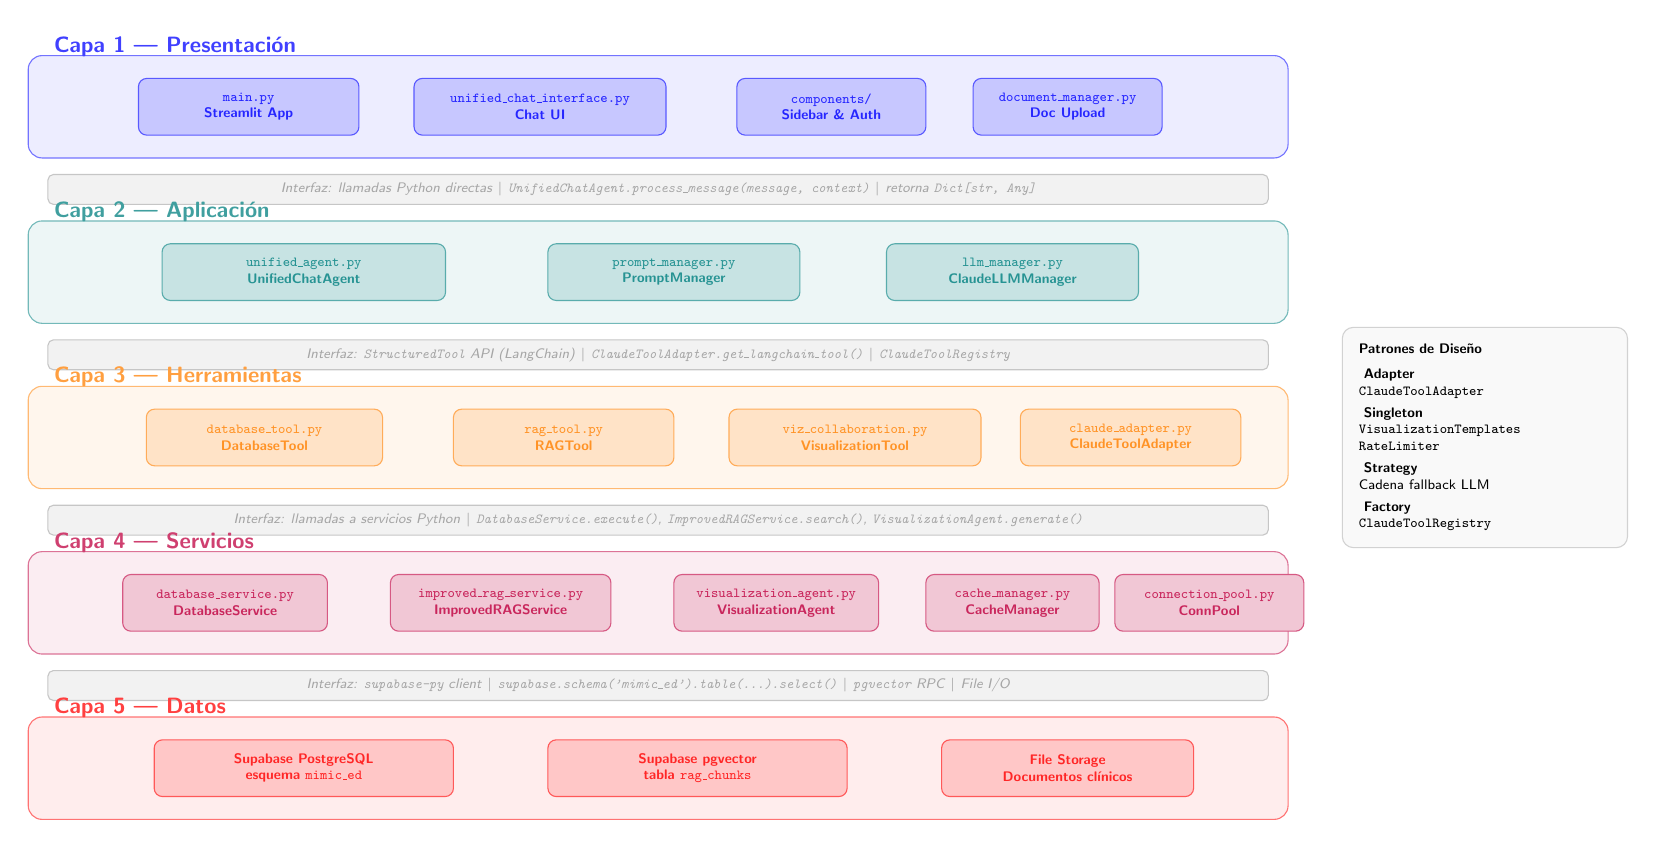
\begin{tikzpicture}[
  layerbox/.style={
    draw=#1!55, fill=#1!7, rounded corners=5pt,
    minimum width=16cm, inner sep=7pt,
    font=\footnotesize\sffamily
  },
  compbox/.style={
    draw=#1!65, fill=#1!22, rounded corners=3pt,
    minimum height=0.72cm, font=\tiny\sffamily\bfseries,
    text=#1!85, align=center, inner sep=3pt
  },
  ifacebox/.style={
    draw=gray!45, fill=gray!10, rounded corners=2pt,
    minimum height=0.38cm, font=\tiny\sffamily\itshape,
    text=gray!70, align=center, inner sep=2pt
  },
  layerlabel/.style={
    font=\footnotesize\sffamily\bfseries, text=#1!75
  },
  patternbadge/.style={
    draw=#1!60, fill=#1!15, rounded corners=8pt,
    font=\tiny\sffamily\bfseries, text=#1!80,
    inner sep=2pt, minimum height=0.35cm
  }
]

% ---- Capa 1: Presentación ----
\node[layerbox=blue, minimum height=1.3cm] (L1) at (0, 0) {};
\node[layerlabel=blue, anchor=west] at ([xshift=6pt, yshift=3pt]L1.north west) {Capa 1 — Presentación};
\node[compbox=blue, minimum width=2.8cm] at (-5.2, 0) {\texttt{main.py}\\Streamlit App};
\node[compbox=blue, minimum width=3.2cm] at (-1.5, 0) {\texttt{unified\_chat\_interface.py}\\Chat UI};
\node[compbox=blue, minimum width=2.4cm] at (2.2, 0) {\texttt{components/}\\Sidebar \& Auth};
\node[compbox=blue, minimum width=2.4cm] at (5.2, 0) {\texttt{document\_manager.py}\\Doc Upload};

% ---- Interfaz 1→2 ----
\node[ifacebox, minimum width=15.5cm] (I12) at (0, -1.05) {Interfaz: llamadas Python directas $\mid$ \texttt{UnifiedChatAgent.process\_message(message, context)} $\mid$ retorna \texttt{Dict[str, Any]}};

% ---- Capa 2: Aplicación ----
\node[layerbox=teal, minimum height=1.3cm] (L2) at (0, -2.1) {};
\node[layerlabel=teal, anchor=west] at ([xshift=6pt, yshift=3pt]L2.north west) {Capa 2 — Aplicación};
\node[compbox=teal, minimum width=3.6cm] at (-4.5, -2.1) {\texttt{unified\_agent.py}\\UnifiedChatAgent};
\node[compbox=teal, minimum width=3.2cm] at (0.2, -2.1) {\texttt{prompt\_manager.py}\\PromptManager};
\node[compbox=teal, minimum width=3.2cm] at (4.5, -2.1) {\texttt{llm\_manager.py}\\ClaudeLLMManager};

% ---- Interfaz 2→3 ----
\node[ifacebox, minimum width=15.5cm] (I23) at (0, -3.15) {Interfaz: \texttt{StructuredTool} API (LangChain) $\mid$ \texttt{ClaudeToolAdapter.get\_langchain\_tool()} $\mid$ \texttt{ClaudeToolRegistry}};

% ---- Capa 3: Herramientas ----
\node[layerbox=orange, minimum height=1.3cm] (L3) at (0, -4.2) {};
\node[layerlabel=orange, anchor=west] at ([xshift=6pt, yshift=3pt]L3.north west) {Capa 3 — Herramientas};
\node[compbox=orange, minimum width=3.0cm] at (-5.0, -4.2) {\texttt{database\_tool.py}\\DatabaseTool};
\node[compbox=orange, minimum width=2.8cm] at (-1.2, -4.2) {\texttt{rag\_tool.py}\\RAGTool};
\node[compbox=orange, minimum width=3.2cm] at (2.5, -4.2) {\texttt{viz\_collaboration.py}\\VisualizationTool};
\node[compbox=orange, minimum width=2.8cm] at (6.0, -4.2) {\texttt{claude\_adapter.py}\\ClaudeToolAdapter};

% ---- Interfaz 3→4 ----
\node[ifacebox, minimum width=15.5cm] (I34) at (0, -5.25) {Interfaz: llamadas a servicios Python $\mid$ \texttt{DatabaseService.execute()}, \texttt{ImprovedRAGService.search()}, \texttt{VisualizationAgent.generate()}};

% ---- Capa 4: Servicios ----
\node[layerbox=purple, minimum height=1.3cm] (L4) at (0, -6.3) {};
\node[layerlabel=purple, anchor=west] at ([xshift=6pt, yshift=3pt]L4.north west) {Capa 4 — Servicios};
\node[compbox=purple, minimum width=2.6cm] at (-5.5, -6.3) {\texttt{database\_service.py}\\DatabaseService};
\node[compbox=purple, minimum width=2.8cm] at (-2.0, -6.3) {\texttt{improved\_rag\_service.py}\\ImprovedRAGService};
\node[compbox=purple, minimum width=2.6cm] at (1.5, -6.3) {\texttt{visualization\_agent.py}\\VisualizationAgent};
\node[compbox=purple, minimum width=2.2cm] at (4.5, -6.3) {\texttt{cache\_manager.py}\\CacheManager};
\node[compbox=purple, minimum width=2.4cm] at (7.0, -6.3) {\texttt{connection\_pool.py}\\ConnPool};

% ---- Interfaz 4→5 ----
\node[ifacebox, minimum width=15.5cm] (I45) at (0, -7.35) {Interfaz: \texttt{supabase-py} client $\mid$ \texttt{supabase.schema('mimic\_ed').table(...).select()} $\mid$ \texttt{pgvector} RPC $\mid$ File I/O};

% ---- Capa 5: Datos ----
\node[layerbox=red, minimum height=1.3cm] (L5) at (0, -8.4) {};
\node[layerlabel=red, anchor=west] at ([xshift=6pt, yshift=3pt]L5.north west) {Capa 5 — Datos};
\node[compbox=red, minimum width=3.8cm] at (-4.5, -8.4) {Supabase PostgreSQL\\esquema \texttt{mimic\_ed}};
\node[compbox=red, minimum width=3.8cm] at (0.5, -8.4) {Supabase pgvector\\tabla \texttt{rag\_chunks}};
\node[compbox=red, minimum width=3.2cm] at (5.2, -8.4) {File Storage\\Documentos clínicos};

% ---- Leyenda de patrones (derecha) ----
\node[draw=gray!35, fill=gray!5, rounded corners=4pt, inner sep=6pt,
      font=\tiny\sffamily, align=left, text width=3.2cm] at (10.5, -4.2)
  {\textbf{Patrones de Diseño}\\[3pt]
   \textcolor{orange!80}{$\blacksquare$} \textbf{Adapter}\\
   \texttt{ClaudeToolAdapter}\\[2pt]
   \textcolor{purple!80}{$\blacksquare$} \textbf{Singleton}\\
   \texttt{VisualizationTemplates}\\
   \texttt{RateLimiter}\\[2pt]
   \textcolor{teal!80}{$\blacksquare$} \textbf{Strategy}\\
   Cadena fallback LLM\\[2pt]
   \textcolor{blue!80}{$\blacksquare$} \textbf{Factory}\\
   \texttt{ClaudeToolRegistry}};

\end{tikzpicture}
\caption{Arquitectura por capas de ChatHCE con interfaces entre capas y patrones de diseño. Las interfaces definen los contratos entre capas adyacentes; ninguna capa puede saltarse una capa intermedia para acceder a otra.}
\label{fig:capas_interfaces}
\end{figure*}

\subsubsection{Descripción de las Cinco Capas}

\textbf{Capa 1 — Presentación.} Implementada íntegramente con Streamlit, gestiona la interfaz de usuario sin contener lógica de negocio. Sus componentes son: \texttt{main.py} (punto de entrada de la aplicación), \texttt{unified\_chat\_interface.py} (interfaz de chat con renderizado de mensajes, visualizaciones y fuentes), y el directorio \texttt{components/} (sidebar de navegación, páginas de autenticación, gestor de documentos). Esta capa recibe eventos del usuario y delega todo el procesamiento a la capa de aplicación mediante llamadas Python directas. Su aislamiento permite sustituir Streamlit por otro framework de UI sin modificar ninguna capa inferior.

\textbf{Capa 2 — Aplicación.} Contiene la lógica de orquestación del sistema. El \texttt{UnifiedChatAgent} (\texttt{unified\_agent.py}) es el componente central: recibe la consulta del usuario, gestiona el historial conversacional (hasta 150K tokens), invoca el \texttt{AgentExecutor} de LangChain y sintetiza la respuesta final. El \texttt{PromptManager} (\texttt{prompt\_manager.py}) genera y cachea el prompt del sistema bajo un límite de 4000 tokens, con caché independiente por sección. El \texttt{ClaudeLLMManager} (\texttt{llm\_manager.py}) gestiona la cadena de fallback de modelos y los reintentos con backoff exponencial. Esta capa aplica el patrón \textit{Strategy} para la selección de modelos.

\textbf{Capa 3 — Herramientas.} Tres herramientas especializadas adaptadas al formato de LangChain mediante el patrón \textit{Adapter}: \texttt{DatabaseTool} (\texttt{database\_tool.py}) para consultas SQL sobre MIMIC-IV-ED, \texttt{RAGTool} (\texttt{rag\_tool.py}) para búsqueda semántica en documentos clínicos, y \texttt{VisualizationTool} (\texttt{viz\_collaboration.py}) para generación de gráficas. La clase abstracta \texttt{ClaudeToolAdapter} (\texttt{claude\_adapter.py}) define la interfaz común que todas las herramientas deben implementar, y el \texttt{ClaudeToolRegistry} aplica el patrón \textit{Factory} para su registro y recuperación centralizada.

\textbf{Capa 4 — Servicios.} Servicios de infraestructura que encapsulan el acceso a recursos externos: \texttt{DatabaseService} (\texttt{database\_service.py}) con validación SQL multicapa y decorador \texttt{@retry\_on\_failure}, \texttt{ImprovedRAGService} (\texttt{improved\_rag\_service.py}) con pipeline de búsqueda híbrida y reranking, \texttt{VisualizationAgent} (\texttt{visualization\_agent.py}) con inicialización \textit{lazy} y enfoque \textit{template-first}, \texttt{CacheManager} (\texttt{cache\_manager.py}) con política LRU y TTL configurable, y el gestor de pool de conexiones (\texttt{connection\_pool\_manager.py}). Esta capa aplica el patrón \textit{Singleton} en \texttt{VisualizationTemplates} y \texttt{RateLimiter}.

\textbf{Capa 5 — Datos.} Backend de datos unificado en Supabase: PostgreSQL con el esquema \texttt{mimic\_ed} (6 tablas MIMIC-IV-ED), Supabase pgvector con la tabla \texttt{rag\_chunks} (embeddings de 384 dimensiones con índice HNSW), y almacenamiento de archivos para documentos clínicos indexados. El acceso se realiza exclusivamente mediante el cliente Python \texttt{supabase-py}, con especificación obligatoria de esquema para tablas clínicas.

\subsubsection{Patrones de Diseño Aplicados}

\textbf{Adapter} (\texttt{ClaudeToolAdapter}). Problema: las tres herramientas del sistema tienen interfaces heterogéneas (SQL, búsqueda vectorial, generación de código), pero LangChain requiere que todas implementen la interfaz \texttt{StructuredTool}. Solución: la clase abstracta \texttt{ClaudeToolAdapter} define los métodos \texttt{execute()}, \texttt{format\_input()}, \texttt{format\_output()} y \texttt{get\_langchain\_tool()}, que cada herramienta implementa. Beneficio: añadir una nueva herramienta requiere únicamente implementar esta interfaz, sin modificar el agente.

\textbf{Singleton} (\texttt{VisualizationTemplates}, \texttt{RateLimiter}). Problema: las plantillas de visualización y el estado del rate limiter deben ser compartidos entre todas las instancias del sistema sin duplicación. Solución: ambas clases implementan el patrón Singleton con \texttt{\_instance = None} y \texttt{\_\_new\_\_} sobrescrito. Beneficio: estado compartido consistente y ahorro de memoria.

\textbf{Strategy} (cadena de fallback LLM). Problema: el modelo LLM óptimo puede variar en tiempo de ejecución según disponibilidad y carga. Solución: \texttt{ClaudeLLMManager} mantiene una lista ordenada de configuraciones de modelos (\texttt{self.models}) y el método \texttt{switch\_to\_fallback()} intercambia el algoritmo (modelo) en tiempo de ejecución sin modificar el código cliente. Beneficio: alta disponibilidad sin cambios en la lógica del agente.

\textbf{Factory} (\texttt{ClaudeToolRegistry}). Problema: la creación y registro de herramientas debe estar centralizada para facilitar la extensibilidad. Solución: el \texttt{ClaudeToolRegistry} actúa como fábrica centralizada que registra herramientas por nombre y las recupera bajo demanda. Las funciones \texttt{create\_database\_tool()}, \texttt{create\_rag\_tool()} y \texttt{create\_visualization\_collaboration\_tool()} encapsulan la lógica de construcción. Beneficio: el agente no necesita conocer los detalles de construcción de cada herramienta.

% ============================================================================
\subsection{Decisiones de Diseño Justificadas}
\label{sec:decisiones_diseno}
% ============================================================================

Esta sección documenta las cinco decisiones arquitectónicas más relevantes de ChatHCE siguiendo el formato \textit{Architecture Decision Record} (ADR) \citep{Nygard2011}: \textbf{[Problema]} $\rightarrow$ \textbf{[Alternativas]} $\rightarrow$ \textbf{[Decisión]} $\rightarrow$ \textbf{[Justificación]}. Este formato garantiza que las decisiones sean trazables, reproducibles y auditables, demostrando que no fueron arbitrarias sino el resultado de un análisis razonado de alternativas.

% ---- Decisión 1 ----
\begin{tcolorbox}[
  enhanced, breakable,
  colback=blue!4, colframe=blue!45,
  title={\footnotesize\sffamily\bfseries Decisión 1 — Supabase como backend unificado (vs.\ servicios separados)},
  fonttitle=\color{white},
  attach boxed title to top left={yshift=-2mm, xshift=4mm},
  boxed title style={colback=blue!55, rounded corners},
  left=4pt, right=4pt, top=4pt, bottom=4pt
]
\footnotesize
\textbf{Problema:} El sistema requiere simultáneamente almacenamiento relacional (datos MIMIC-IV-ED), almacén vectorial (embeddings RAG), autenticación de usuarios y API REST. Gestionar tres o cuatro servicios independientes introduce complejidad operacional y latencia de red entre ellos.

\textbf{Alternativas consideradas:}
\begin{itemize}[nosep, leftmargin=*]
  \item PostgreSQL + Pinecone + Auth0 (tres servicios separados, tres SDKs, tres puntos de fallo)
  \item MongoDB Atlas + Weaviate (sin soporte SQL nativo, sin búsqueda híbrida integrada)
  \item Firebase + Chroma (sin PostgreSQL completo, sin funciones de ventana para análisis temporal)
\end{itemize}

\textbf{Decisión adoptada:} Supabase (PostgreSQL 15 + pgvector 0.8.0 + Supabase Auth).

\textbf{Justificación técnica:} La búsqueda híbrida vectorial-léxica se ejecuta como una única función RPC de PostgreSQL, eliminando la latencia de red entre un servicio vectorial externo y la base de datos relacional. Un solo punto de autenticación con Row Level Security (RLS) aplica políticas de acceso uniformes sobre las 13 tablas del sistema. PostgREST genera automáticamente la API REST sin código adicional. La superficie de ataque se reduce a un único servicio frente a tres con sus propias vulnerabilidades y configuraciones de seguridad independientes. Evidencia en código: \texttt{services/medical\_agent/services/database\_service.py} accede a ambos esquemas (\texttt{mimic\_ed} y \texttt{public}) mediante el mismo cliente \texttt{supabase-py}, y la función RPC \texttt{hybrid\_search} en \texttt{services/rag/supabase\_vector\_store.py} combina pgvector y tsvector en una sola llamada.
\end{tcolorbox}

% ---- Decisión 2 ----
\begin{tcolorbox}[
  enhanced, breakable,
  colback=teal!4, colframe=teal!45,
  title={\footnotesize\sffamily\bfseries Decisión 2 — Chunking jerárquico padre-hijo (vs.\ chunking uniforme)},
  fonttitle=\color{white},
  attach boxed title to top left={yshift=-2mm, xshift=4mm},
  boxed title style={colback=teal!55, rounded corners},
  left=4pt, right=4pt, top=4pt, bottom=4pt
]
\footnotesize
\textbf{Problema:} Existe un \textit{trade-off} fundamental en RAG entre granularidad para búsqueda precisa y contexto suficiente para generación de respuestas. Los chunks pequeños mejoran la precisión de recuperación pero truncan el contexto clínico; los chunks grandes preservan el contexto pero degradan la precisión semántica.

\textbf{Alternativas consideradas:}
\begin{itemize}[nosep, leftmargin=*]
  \item Chunking fijo de 512 tokens (estándar, pero pierde contexto en guías con dosis y protocolos)
  \item Chunking por párrafo (tamaño variable, difícil de controlar)
  \item Chunking por oración (demasiado granular para embeddings de 384 dimensiones)
\end{itemize}

\textbf{Decisión adoptada:} Chunks hijo de 400 caracteres para búsqueda + expansión a chunks padre de 1500 caracteres para contexto, implementado en \texttt{services/rag/parent\_child\_chunker.py}.

\textbf{Justificación técnica:} Los bi-encoders de 384 dimensiones como \texttt{all-MiniLM-L6-v2} capturan mejor la semántica en fragmentos cortos \citep{Wang2020}. La expansión al chunk padre garantiza que el LLM recibe contexto clínico completo sin truncar oraciones a mitad, especialmente relevante para guías con dosificaciones y protocolos de urgencias donde la continuidad del texto es crítica. La columna \texttt{parent\_id} en \texttt{rag\_chunks} implementa la expansión con una sola query SQL JOIN, sin overhead adicional. Los parámetros \texttt{CHILD\_CHUNK\_SIZE = 400} y \texttt{PARENT\_CHUNK\_SIZE = 1500} están configurados en \texttt{services/rag/parent\_child\_chunker.py}.
\end{tcolorbox}

% ---- Decisión 3 ----
\begin{tcolorbox}[
  enhanced, breakable,
  colback=purple!4, colframe=purple!45,
  title={\footnotesize\sffamily\bfseries Decisión 3 — Búsqueda híbrida vectorial-léxica con RRF (vs.\ búsqueda vectorial pura)},
  fonttitle=\color{white},
  attach boxed title to top left={yshift=-2mm, xshift=4mm},
  boxed title style={colback=purple!55, rounded corners},
  left=4pt, right=4pt, top=4pt, bottom=4pt
]
\footnotesize
\textbf{Problema:} La búsqueda vectorial pura falla en términos médicos exactos. Códigos ICD como \texttt{I48.91} (fibrilación auricular), nombres de fármacos como \texttt{metoprolol 25mg} o dosificaciones específicas no tienen buena cobertura semántica en embeddings genéricos entrenados sobre texto general.

\textbf{Alternativas consideradas:}
\begin{itemize}[nosep, leftmargin=*]
  \item Búsqueda vectorial pura (similitud coseno): falla en términos exactos y acrónimos médicos
  \item BM25 pura: no captura sinónimos ni variantes semánticas
  \item ElasticSearch: servicio externo adicional, latencia de red, coste operacional
\end{itemize}

\textbf{Decisión adoptada:} pgvector (similitud coseno) + tsvector (full-text search en español) + Reciprocal Rank Fusion (RRF), ejecutado como función RPC en PostgreSQL.

\textbf{Justificación técnica:} La búsqueda léxica con stemming en español (\texttt{tsvector} con configuración \texttt{spanish}) mejora el recall para variantes morfológicas de términos médicos. RRF combina los rankings de ambas búsquedas sin requerir calibración de pesos, usando la fórmula $\text{RRF}(d) = \sum_{r \in R} \frac{1}{k + r(d)}$ con $k=60$ \citep{Cormack2009}. Todo se ejecuta como función RPC de PostgreSQL, con latencia media medida inferior a 500 ms. Evidencia en código: función \texttt{hybrid\_search} en \texttt{services/rag/supabase\_vector\_store.py} y columna generada \texttt{fts tsvector} en la tabla \texttt{rag\_chunks}.
\end{tcolorbox}

% ---- Decisión 4 ----
\begin{tcolorbox}[
  enhanced, breakable,
  colback=orange!4, colframe=orange!45,
  title={\footnotesize\sffamily\bfseries Decisión 4 — Enfoque template-first en visualización (vs.\ generación LLM para todo)},
  fonttitle=\color{white},
  attach boxed title to top left={yshift=-2mm, xshift=4mm},
  boxed title style={colback=orange!55, rounded corners},
  left=4pt, right=4pt, top=4pt, bottom=4pt
]
\footnotesize
\textbf{Problema:} La generación de código Plotly por LLM introduce latencia de $\sim$4 segundos y no-determinismo: el mismo tipo de gráfica puede producir código diferente en cada invocación, con riesgo de errores de ejecución.

\textbf{Alternativas consideradas:}
\begin{itemize}[nosep, leftmargin=*]
  \item LLM para todos los casos: máxima flexibilidad pero latencia alta y no-determinismo
  \item Librería predefinida sin LLM: latencia mínima pero sin flexibilidad para casos atípicos
\end{itemize}

\textbf{Decisión adoptada:} 12+ plantillas Plotly predefinidas en \texttt{VisualizationTemplates} (Singleton) + fallback a Claude Sonnet 4.5 (\texttt{claude-sonnet-4-5}) para casos no cubiertos.

\textbf{Justificación técnica:} Las visualizaciones clínicas habituales son predecibles: timeline de signos vitales, distribuciones de diagnósticos, comparativas entre pacientes, indicadores de triaje. Las plantillas reducen la latencia de $\sim$4 s a $\sim$0.4 s en el 90\% de los casos. El fallback al LLM garantiza flexibilidad para visualizaciones atípicas. La inicialización \textit{lazy} del \texttt{VisualizationAgent} (\texttt{services/medical\_agent/visualization\_agent.py}) ahorra memoria en el 90\% de las consultas que no requieren generación LLM. El \texttt{VisualizationSelector} (\texttt{services/medical\_agent/visualization\_selector.py}) analiza las características de los datos (tipos de columnas, cardinalidad, presencia de series temporales) para seleccionar automáticamente la plantilla apropiada.
\end{tcolorbox}

% ---- Decisión 5 (Central) ----
\begin{tcolorbox}[
  enhanced, breakable,
  colback=orange!6, colframe=orange!60,
  title={\small\sffamily\bfseries\color{white} Decisión Arquitectónica Central — Agente Unificado vs.\ Arquitectura Multi-Agente},
  attach boxed title to top left={yshift=-2mm, xshift=4mm},
  boxed title style={colback=orange!70, rounded corners},
  left=5pt, right=5pt, top=5pt, bottom=5pt
]
\footnotesize
\textbf{Problema:} Elegir entre un agente conversacional unificado y una arquitectura multi-agente con agentes especializados para cada dominio (base de datos, RAG, visualización, crítica).

\textbf{Alternativas consideradas:}
\begin{itemize}[nosep, leftmargin=*]
  \item \textbf{Multi-agente con LangGraph}: grafo DAG con \texttt{OrchestratorAgent} $\rightarrow$ [\texttt{DBAgent}, \texttt{RAGAgent}, \texttt{VizAgent}] $\rightarrow$ \texttt{CriticAgent}. Mayor paralelización pero latencia acumulada y error propagado entre nodos.
  \item \textbf{Multi-agente con CrewAI}: roles especializados (médico, buscador, crítico). Mayor expresividad semántica pero complejidad de coordinación y coste de múltiples llamadas LLM por turno.
  \item \textbf{Agente único sin herramientas}: prompt gigante sin tool-calling. Sin latencia de coordinación pero sin acceso a datos reales, inaceptable para un sistema clínico.
\end{itemize}

\textbf{Decisión adoptada:} Agente unificado (\texttt{UnifiedChatAgent}) con tool-calling nativo de Claude Haiku 4.5, implementado en \texttt{services/unified\_chat/unified\_agent.py}.

\textbf{Justificación técnica:}
\begin{itemize}[nosep, leftmargin=*]
  \item \textbf{Menor latencia}: una sola llamada LLM por turno de conversación frente a 3-5 llamadas en arquitecturas multi-agente. El \texttt{AgentExecutor} con \texttt{max\_iterations=5} y \texttt{max\_execution\_time=120} garantiza un límite superior de tiempo.
  \item \textbf{Menor error acumulado}: en cadenas de agentes, cada paso puede propagar errores o malinterpretaciones. El agente unificado sintetiza directamente desde los resultados de las herramientas.
  \item \textbf{Capacidad suficiente}: Claude Haiku 4.5 tiene capacidad de razonamiento clínico suficiente para el 95\% de las consultas, como demuestran los resultados de los test cases de evaluación (Sección~\ref{sec:evaluacion}).
  \item \textbf{Tool-calling determinista}: Claude genera directamente el nombre de la herramienta y los parámetros en JSON, sin simulación mediante prompts. El método \texttt{create\_tool\_calling\_agent(llm, tools, prompt)} de LangChain aprovecha esta capacidad nativa.
  \item \textbf{Fallback elegante}: la cadena Haiku $\rightarrow$ Sonnet $\rightarrow$ Opus proporciona la escalabilidad que normalmente se busca con multi-agente, pero con menor complejidad arquitectónica.
\end{itemize}

\textbf{Trade-offs asumidos:} Se pierde la paralelización de agentes (mitigado porque las herramientas son rápidas: P50 $<$ 2 s) y la revisión crítica autónoma (mitigado por las directivas anti-alucinación en el prompt del sistema, Sección~\ref{sec:antihallucination_37}).
\end{tcolorbox}

La Figura~\ref{fig:agente_vs_multiagente} ilustra visualmente la comparativa entre la arquitectura multi-agente descartada y el agente unificado adoptado.

\begin{figure*}[t]
\centering
\begin{tikzpicture}[
  agentnode/.style={
    draw=#1!65, fill=#1!12, rounded corners=4pt,
    minimum width=2.6cm, minimum height=0.7cm,
    font=\small\sffamily, text=#1!80, align=center
  },
  toolnode/.style={
    draw=#1!60, fill=#1!18, rounded corners=3pt,
    minimum width=2.2cm, minimum height=0.6cm,
    font=\small\sffamily\bfseries, text=#1!80, align=center
  },
  disadvlabel/.style={
    font=\tiny\sffamily\itshape, text=accent!70, align=center
  },
  advlabel/.style={
    font=\tiny\sffamily\itshape, text=success!70, align=center
  },
  flowarrow/.style={
    -{Stealth[length=5pt]}, thick, color=#1!60
  }
]

% ===== COLUMNA IZQUIERDA: Multi-Agente (descartado) =====
\node[font=\small\sffamily\bfseries, text=gray!60] at (-5.5, 4.5) {Arquitectura Multi-Agente};
\node[font=\tiny\sffamily\itshape, text=gray!50] at (-5.5, 4.1) {(alternativa descartada)};

\node[agentnode=gray, minimum width=3.0cm] (orch) at (-5.5, 3.2) {OrchestratorAgent};
\node[agentnode=gray, minimum width=2.4cm] (dba) at (-7.5, 1.8) {DBAgent};
\node[agentnode=gray, minimum width=2.4cm] (raga) at (-5.5, 1.8) {RAGAgent};
\node[agentnode=gray, minimum width=2.4cm] (viza) at (-3.5, 1.8) {VizAgent};
\node[agentnode=gray, minimum width=3.0cm] (critic) at (-5.5, 0.4) {CriticAgent};
\node[agentnode=gray, minimum width=3.0cm] (resp1) at (-5.5, -0.8) {Respuesta};

\draw[flowarrow=gray] (orch) -- (dba);
\draw[flowarrow=gray] (orch) -- (raga);
\draw[flowarrow=gray] (orch) -- (viza);
\draw[flowarrow=gray] (dba) |- (critic);
\draw[flowarrow=gray] (raga) -- (critic);
\draw[flowarrow=gray] (viza) |- (critic);
\draw[flowarrow=gray] (critic) -- (resp1);

% Etiquetas de desventajas
\node[disadvlabel] at (-5.5, -1.5) {$\times$ 3--5 llamadas LLM por turno};
\node[disadvlabel] at (-5.5, -1.9) {$\times$ Error acumulado entre nodos};
\node[disadvlabel] at (-5.5, -2.3) {$\times$ Complejidad de coordinación};
\node[disadvlabel] at (-5.5, -2.7) {$\times$ Latencia $>$ 10 s (estimada)};

% Cruz roja
\node[font=\Large\bfseries, text=accent] at (-5.5, 5.0) {$\times$};

% ===== SEPARADOR CENTRAL =====
\draw[very thick, gray!30, dashed] (0, -3.2) -- (0, 5.2);
\node[font=\large\sffamily\bfseries, text=gray!50] at (0, 1.2) {vs.};

% ===== COLUMNA DERECHA: Agente Unificado (adoptado) =====
\node[font=\small\sffamily\bfseries, text=success!70] at (5.5, 4.5) {Agente Unificado ChatHCE};
\node[font=\tiny\sffamily\itshape, text=success!50] at (5.5, 4.1) {(decisión adoptada)};

\node[agentnode=success, minimum width=3.8cm] (unified) at (5.5, 3.2) {UnifiedChatAgent\\Claude Haiku 4.5};

\node[toolnode=dbcolor, minimum width=2.2cm] (dbt) at (3.5, 1.8) {DB Tool};
\node[toolnode=ragcolor, minimum width=2.2cm] (ragt) at (5.5, 1.8) {RAG Tool};
\node[toolnode=vizcolor, minimum width=2.2cm] (vizt) at (7.5, 1.8) {VIZ Tool};

\node[agentnode=success, minimum width=3.8cm] (synth) at (5.5, 0.4) {Síntesis directa\\(una sola llamada LLM)};
\node[agentnode=success, minimum width=3.8cm] (resp2) at (5.5, -0.8) {Respuesta integrada};

\draw[flowarrow=success] (unified) -- (dbt);
\draw[flowarrow=success] (unified) -- (ragt);
\draw[flowarrow=success] (unified) -- (vizt);
\draw[flowarrow=dbcolor] (dbt) |- (synth);
\draw[flowarrow=ragcolor] (ragt) -- (synth);
\draw[flowarrow=vizcolor] (vizt) |- (synth);
\draw[flowarrow=success] (synth) -- (resp2);

% Cadena de fallback
\node[draw=accent!50, fill=accent!8, rounded corners=3pt,
      font=\tiny\sffamily, align=center, inner sep=3pt,
      minimum width=2.8cm] (fallback) at (9.5, 3.2)
  {Fallback:\\Haiku $\rightarrow$ Sonnet\\$\rightarrow$ Opus};
\draw[dashedarrow, color=accent!50] (unified.east) -- (fallback.west);

% Etiquetas de ventajas
\node[advlabel] at (5.5, -1.5) {$\checkmark$ 1 llamada LLM por turno};
\node[advlabel] at (5.5, -1.9) {$\checkmark$ Sin error acumulado};
\node[advlabel] at (5.5, -2.3) {$\checkmark$ Fallback elegante integrado};
\node[advlabel] at (5.5, -2.7) {$\checkmark$ Latencia P50 $<$ 5 s (medida)};

% Check verde
\node[font=\Large\bfseries, text=success] at (5.5, 5.0) {$\checkmark$};

\end{tikzpicture}
\caption{Comparativa entre la arquitectura multi-agente descartada (izquierda) y el agente unificado adoptado (derecha). El agente unificado reduce la latencia, elimina el error acumulado entre nodos y simplifica la arquitectura sin sacrificar capacidad de razonamiento clínico.}
\label{fig:agente_vs_multiagente}
\end{figure*}

% ============================================================================
\subsection{Arquitectura del Agente y Selección de Herramientas}
\label{sec:arquitectura_agente}
% ============================================================================

\subsubsection{El Ciclo ReAct del Agente}
\label{sec:react}

El \texttt{UnifiedChatAgent} implementa el patrón \textbf{ReAct} (\textit{Reasoning + Acting}) \citep{Yao2022}, que intercala razonamiento en lenguaje natural con acciones concretas sobre herramientas externas. A diferencia de los enfoques que separan el razonamiento de la acción, ReAct permite que el modelo actualice su plan de acción en función de las observaciones obtenidas de las herramientas, produciendo respuestas más precisas y fundamentadas en datos reales.

El ciclo ReAct en ChatHCE se articula en cuatro fases iterativas, gestionadas por el \texttt{AgentExecutor} de LangChain con \texttt{max\_iterations=5} y \texttt{max\_execution\_time=120} segundos:

\begin{enumerate}[nosep, leftmargin=*]
  \item \textbf{Think}: Claude Haiku 4.5 analiza la consulta del usuario, el historial conversacional y el contexto de datos previos inyectado por \texttt{\_enrich\_message\_with\_context()}. Determina qué herramientas invocar y con qué parámetros.
  \item \textbf{Act}: El modelo genera directamente el nombre de la herramienta y los parámetros en JSON mediante tool-calling nativo (no simulado con prompts). La función \texttt{create\_tool\_calling\_agent(llm, tools, prompt)} de LangChain aprovecha esta capacidad nativa de Claude.
  \item \textbf{Observe}: El \texttt{AgentExecutor} ejecuta la herramienta seleccionada y devuelve el resultado al modelo. Los resultados intermedios se almacenan en \texttt{return\_intermediate\_steps=True} para trazabilidad.
  \item \textbf{Synthesize}: Claude integra los resultados de todas las herramientas invocadas y genera la respuesta final en español, con citación de fuentes y reconocimiento explícito de incertidumbre según las directivas anti-alucinación.
\end{enumerate}

La Figura~\ref{fig:react_cycle} muestra el ciclo interno completo del agente con las tres herramientas y la cadena de fallback.

\subsubsection{Las Tres Herramientas Especializadas}
\label{sec:herramientas}

\textbf{DatabaseTool} (\texttt{query\_mimic\_database}). Recibe una consulta en lenguaje natural que el agente traduce a parámetros estructurados según el esquema Pydantic \texttt{DatabaseToolInput}. Los campos del esquema son: \texttt{query\_type} (tipos: \texttt{patient\_summary}, \texttt{vital\_signs}, \texttt{diagnoses}, \texttt{medications}, \texttt{custom}), \texttt{subject\_id} (INT, opcional), \texttt{stay\_id} (INT, opcional), \texttt{icd\_code} (VARCHAR, opcional), \texttt{custom\_query} (SQL validado, opcional) y \texttt{limit} (INT, máximo 5000, por defecto 1000). La herramienta delega en \texttt{DatabaseService} para la ejecución, aplicando validación SQL multicapa antes de cada consulta. Retorna un \texttt{Dict} con \texttt{success}, \texttt{data}, \texttt{query\_type}, \texttt{parameters} y \texttt{count}.

\textbf{RAGTool} (\texttt{search\_clinical\_documents}). Recibe una consulta clínica en lenguaje natural. Internamente, el \texttt{QueryAugmenter} genera hasta 3 consultas alternativas mediante Multi-Query y HyDE (Hypothetical Document Embeddings) \citep{Gao2022}. La búsqueda híbrida recupera los $k$ chunks más relevantes (por defecto $k=5$) con sus puntuaciones de similitud $s_i \in [0,1]$. El \texttt{Reranker} reordena los resultados con \texttt{cross-encoder/ms-marco-MiniLM-L-6-v2}. Retorna los chunks con metadatos de fuente (\texttt{filename}, \texttt{specialty}, \texttt{document\_type}) para citación obligatoria.

\textbf{VisualizationTool} (\texttt{request\_visualization}). Recibe los datos clínicos y el tipo de gráfica solicitado. El \texttt{DataPreprocessor} limpia y valida los datos (máximo 5000 puntos). El \texttt{VisualizationSelector} selecciona la plantilla apropiada entre 12+ tipos: \texttt{timeline}, \texttt{comparison}, \texttt{histogram}, \texttt{scatter}, \texttt{bar}, \texttt{box}, \texttt{violin}, \texttt{heatmap}, \texttt{pie}, \texttt{sunburst}, \texttt{table} e \texttt{indicator}. Si no existe plantilla adecuada, el \texttt{VisualizationAgent} (inicialización \textit{lazy}) genera código Python con Claude Sonnet 4.5. El \texttt{CodeValidator} valida el código mediante AST antes de la ejecución en sandbox. Retorna la figura en formato base64 PNG o HTML interactivo. En caso de error, la herramienta retorna un mensaje descriptivo sin interrumpir el flujo conversacional.

\subsubsection{La Cadena de Fallback de Modelos}
\label{sec:fallback}

El \texttt{ClaudeLLMManager} implementa una cadena de fallback con tres modelos Claude, configurada en \texttt{config/settings.py} mediante \texttt{ClaudeAgentSettings}:

\begin{itemize}[nosep, leftmargin=*]
  \item \textbf{Modelo primario}: \texttt{claude-haiku-4-5-20251001} — optimizado para velocidad y coste. Parámetros: \texttt{max\_tokens=4096}, \texttt{temperature=0.1}, \texttt{timeout=30 s}.
  \item \textbf{Modelo secundario}: \texttt{claude-sonnet-4-5-20250929} — mayor capacidad de razonamiento. Parámetros: \texttt{max\_tokens=8192}, \texttt{timeout=45 s}.
  \item \textbf{Modelo terciario}: \texttt{claude-opus-4-20250514} — máxima capacidad. Parámetros: \texttt{max\_tokens=4096}, \texttt{timeout=60 s}.
\end{itemize}

El escalado se dispara ante excepciones \texttt{AnthropicRateLimitError} o \texttt{APIError} tras agotar los reintentos del modelo actual. Los parámetros de backoff exponencial son: \texttt{max\_retries=3}, \texttt{retry\_delay=2.0 s}, \texttt{backoff\_multiplier=2.0} (delays: 2 s, 4 s, 8 s). El método \texttt{execute\_with\_retry()} en \texttt{llm\_manager.py} implementa esta lógica, intentando el fallback solo en el último reintento para minimizar la latencia en condiciones normales.

Claude Haiku 4.5 es el modelo primario por su balance entre velocidad ($\sim$800 ms P50 para análisis de intención), coste y capacidad de tool-calling nativo. La temperatura de 0.1 garantiza respuestas deterministas y reproducibles, crítico en un entorno clínico donde la consistencia es prioritaria.

\subsubsection{El Sistema de Prompts y Directivas Anti-Alucinación}
\label{sec:antihallucination_37}

El \texttt{PromptManager} genera el prompt del sistema bajo un límite de 4000 tokens, estructurado en diez secciones con caché independiente por sección (atributos \texttt{schema\_cache}, \texttt{tool\_descriptions\_cache}, \texttt{role\_definition\_cache}, \texttt{response\_format\_cache}, \texttt{clinical\_guidelines\_cache}, \texttt{anti\_hallucination\_cache}, \texttt{full\_prompt\_cache}):

\begin{enumerate}[nosep, leftmargin=*]
  \item \textbf{IDENTIDAD DEL SISTEMA}: rol de ChatHCE y propósito clínico
  \item \textbf{CONTEXTO OPERATIVO}: descripción del dataset MIMIC-IV-ED (222 pacientes, 6 tablas)
  \item \textbf{HERRAMIENTAS DISPONIBLES}: documentación de las tres herramientas con ejemplos
  \item \textbf{DIRECTIVAS ANTI-ALUCINACIÓN}: prohibiciones absolutas y manejo de datos faltantes
  \item \textbf{IDIOMA Y TERMINOLOGÍA}: directivas de respuesta en español médico
  \item \textbf{Base de Datos MIMIC-IV-ED}: esquema condensado con columnas exactas y porcentajes de nulos
  \item \textbf{Herramientas Disponibles}: descripciones detalladas con reglas SQL obligatorias
  \item \textbf{Formato de Respuesta}: estructura recomendada y convenciones de unidades
  \item \textbf{Guías Clínicas}: valores de referencia de signos vitales y niveles de acuidad ESI
  \item \textbf{GUÍAS DE SELECCIÓN DE HERRAMIENTAS}: patrones de detección automática de visualizaciones
\end{enumerate}

Las directivas anti-alucinación (sección 4 del prompt) son la capa de defensa más temprana contra la generación de información clínica falsa. Su implementación en el prompt del sistema, en lugar de como post-procesamiento, es más eficiente: interceptar antes de generar es computacionalmente más barato y más fiable que corregir después de generar. El siguiente bloque reproduce literalmente el núcleo de las directivas, obtenido del método \texttt{get\_anti\_hallucination\_directives()} en \texttt{services/medical\_agent/prompt\_manager.py}:

\begin{tcolorbox}[
  enhanced, breakable,
  colback=accent!4, colframe=accent!50,
  title={\footnotesize\sffamily\bfseries\color{white} Directivas Anti-Alucinación — Extracto del Prompt del Sistema},
  attach boxed title to top left={yshift=-2mm, xshift=4mm},
  boxed title style={colback=accent!60, rounded corners},
  left=4pt, right=4pt, top=4pt, bottom=4pt
]
\begin{lstlisting}[basicstyle=\ttfamily\tiny, backgroundcolor=\color{codebg},
  frame=none, breaklines=true, columns=fullflexible]
# DIRECTIVAS ANTI-ALUCINACION

## PROHIBICIONES ABSOLUTAS - NUNCA HACER

### Identificadores de Pacientes
- NUNCA inventes subject_id (IDs de pacientes)
- NUNCA fabriques stay_id (IDs de estancias)
- NUNCA crees hadm_id (IDs de admision hospitalaria)
- Solo usa identificadores obtenidos de una consulta real a la base de datos

### Valores Clinicos
- NUNCA inventes valores de signos vitales (temperatura, frecuencia cardiaca,
  presion arterial, saturacion O2, frecuencia respiratoria)
- NUNCA fabriques resultados de laboratorio
- Todos los valores numericos deben provenir de consultas reales

### Diagnosticos y Medicamentos
- NUNCA inventes diagnosticos o codigos ICD (ICD-9 o ICD-10)
- NUNCA fabriques nombres de medicamentos
- NUNCA crees dosis o frecuencias de administracion ficticias

## MANEJO DE DATOS FALTANTES
- Si no encuentra datos: "No encontre informacion sobre [X] en el dataset"
- Si hay valores NULL: "Algunos registros tienen datos incompletos para [campo]"
- Si el paciente no existe: "El paciente [ID] no existe en MIMIC-IV-ED"

## CITACION DE FUENTES
- Siempre indica: "Segun los datos obtenidos de la tabla [nombre_tabla]..."
- Cita el documento fuente: "Segun [nombre del documento]..."

## RECONOCIMIENTO DE INCERTIDUMBRE
- Para datos verificados: "Segun los datos disponibles..." / "Los registros muestran..."
- Para interpretaciones: "Esto podria indicar..." / "Una posible interpretacion es..."
- Para inferencias: "Analizando los datos disponibles..."
\end{lstlisting}
\end{tcolorbox}

Las directivas cubren cinco dimensiones complementarias: (1) prohibiciones absolutas de fabricación de identificadores y valores clínicos, (2) protocolos para datos faltantes o nulos, (3) citación obligatoria de fuentes con indicación de tabla y herramienta, (4) diferenciación entre datos verificados e interpretaciones mediante lenguaje condicional, y (5) recordatorio de las limitaciones del dataset (222 pacientes, solo urgencias, fechas desplazadas para anonimización).

\subsubsection{Gestión de Memoria Conversacional}
\label{sec:memoria}

El \texttt{UnifiedChatAgent} gestiona el contexto conversacional con tres mecanismos complementarios:

\textbf{Límite de tokens}: El historial se limita a \texttt{MAX\_HISTORY\_TOKENS = 150\,000} tokens (estimados como $\lfloor\text{chars}/4\rfloor$), reservando espacio para el prompt del sistema ($\sim$10K tokens) y la respuesta ($\sim$4K tokens) dentro del límite de 200K tokens de Claude. Cuando se supera el límite, se eliminan los mensajes más antiguos preservando siempre los \texttt{MIN\_MESSAGES\_TO\_KEEP = 4} mensajes más recientes.

\textbf{Inyección de contexto de datos}: El método \texttt{\_enrich\_message\_with\_context()} añade bloques \texttt{[CONTEXTO DE DATOS]} a los mensajes del asistente, con resúmenes de los resultados de herramientas de interacciones previas. Esto permite al agente referenciar datos consultados anteriormente sin re-ejecutar herramientas, mejorando la eficiencia y la coherencia conversacional. Los mensajes recientes (últimos 3) reciben contexto completo; los mensajes más antiguos reciben solo resúmenes.

\textbf{Trade-off coste-calidad}: Un historial mayor permite consultas de seguimiento más inteligentes (``¿cuál era su presión arterial?'' sin re-ejecutar la herramienta), pero aumenta el coste por token. El límite de 150K tokens representa un equilibrio entre capacidad conversacional y coste operacional, suficiente para conversaciones de hasta $\sim$50 turnos con datos clínicos completos.

% ---- Figura 3.X: Ciclo ReAct del agente ----
\begin{figure*}[t]
\centering
\begin{tikzpicture}[
  phasenode/.style={
    draw=#1!70, fill=#1!14, rounded corners=5pt,
    minimum width=3.2cm, minimum height=1.0cm,
    font=\small\sffamily\bfseries, text=#1!80, align=center,
    drop shadow={shadow xshift=1.5pt, shadow yshift=-1.5pt, fill=#1!20, opacity=0.4}
  },
  toolnode/.style={
    draw=#1!65, fill=#1!18, rounded corners=3pt,
    minimum width=2.6cm, minimum height=0.65cm,
    font=\small\sffamily\bfseries, text=#1!80, align=center
  },
  resultnode/.style={
    draw=#1!55, fill=#1!10, rounded corners=3pt,
    minimum width=2.6cm, minimum height=0.55cm,
    font=\tiny\sffamily, text=#1!75, align=center
  },
  modelnode/.style={
    draw=primary!70, fill=primary!12, rounded corners=6pt,
    minimum width=3.8cm, minimum height=1.4cm,
    font=\small\sffamily\bfseries, text=primary!80, align=center,
    drop shadow={shadow xshift=2pt, shadow yshift=-2pt, fill=primary!20, opacity=0.4}
  },
  fallbacknode/.style={
    draw=accent!55, fill=accent!8, rounded corners=3pt,
    minimum width=2.8cm, minimum height=0.55cm,
    font=\tiny\sffamily, text=accent!75, align=center
  },
  cyclearrow/.style={
    -{Stealth[length=6pt,width=4pt]}, very thick, color=#1!65
  },
  limitlabel/.style={
    draw=gray!35, fill=gray!8, rounded corners=2pt,
    font=\tiny\sffamily\itshape, text=gray!65, inner sep=2pt
  }
]

% ---- Nodo central: Claude Haiku 4.5 ----
\node[modelnode] (claude) at (0, 0) {Claude Haiku 4.5\\(\texttt{claude-haiku-4-5-20251001})\\AgentExecutor};

% ---- Fase THINK (arriba) ----
\node[phasenode=blue] (think) at (0, 3.5) {THINK\\Analiza consulta\\+ historial};
\node[limitlabel] at (3.8, 3.5) {\texttt{max\_iterations=5}\\timeout: 120 s};

% ---- Fase ACT (derecha) ----
\node[phasenode=orange] (act) at (5.5, 0) {ACT\\Tool-calling\\nativo JSON};

% ---- Fase OBSERVE (abajo) ----
\node[phasenode=purple] (observe) at (0, -3.5) {OBSERVE\\Recibe resultados\\de herramientas};

% ---- Fase SYNTHESIZE (izquierda) ----
\node[phasenode=success] (synth) at (-5.5, 0) {SYNTHESIZE\\Integra resultados\\Genera respuesta};

% ---- Flechas del ciclo ----
\draw[cyclearrow=blue] (claude.north) -- (think.south)
  node[midway, right, font=\tiny\sffamily\itshape, text=blue!60] {analiza};
\draw[cyclearrow=orange] (think.east) -- ++(1.5,0) |- (act.north)
  node[near start, above, font=\tiny\sffamily\itshape, text=orange!60] {decide herramientas};
\draw[cyclearrow=orange] (act.south) -- ++(0,-1.0) -| (observe.east)
  node[near start, right, font=\tiny\sffamily\itshape, text=orange!60] {ejecuta};
\draw[cyclearrow=purple] (observe.west) -- ++(-1.5,0) |- (synth.south)
  node[near start, below, font=\tiny\sffamily\itshape, text=purple!60] {resultados};
\draw[cyclearrow=success] (synth.north) -- ++(0,1.0) -| (claude.west)
  node[near start, left, font=\tiny\sffamily\itshape, text=success!60] {respuesta final};

% Flecha de retorno al THINK (nueva iteración)
\draw[cyclearrow=blue, dashed] (synth.north) -- ++(0,2.0) -- (think.west)
  node[midway, above, font=\tiny\sffamily\itshape, text=blue!50] {nueva iteración (si necesario)};

% ---- Herramientas (desde ACT) ----
\node[toolnode=dbcolor] (dbt) at (9.0, 1.8) {DB Tool\\query\_mimic\_database};
\node[toolnode=ragcolor] (ragt) at (9.0, 0) {RAG Tool\\search\_clinical\_documents};
\node[toolnode=vizcolor] (vizt) at (9.0, -1.8) {VIZ Tool\\request\_visualization};

\draw[cyclearrow=dbcolor] (act.east) -- ++(0.5,0) |- (dbt.west);
\draw[cyclearrow=ragcolor] (act.east) -- (ragt.west);
\draw[cyclearrow=vizcolor] (act.east) -- ++(0.5,0) |- (vizt.west);

% ---- Resultados (hacia OBSERVE) ----
\node[resultnode=dbcolor] (dbr) at (9.0, -3.0) {ResultSet SQL\\(Dict + count)};
\node[resultnode=ragcolor] (ragr) at (6.5, -4.5) {Chunks + Scores\\+ Fuentes};
\node[resultnode=vizcolor] (vizr) at (9.0, -5.0) {Plotly Fig\\(base64/HTML)};

\draw[cyclearrow=dbcolor] (dbt.south) -- ++(0,-0.5) -- (dbr.north);
\draw[cyclearrow=ragcolor] (ragt.south) -- ++(0,-1.5) -- (ragr.north);
\draw[cyclearrow=vizcolor] (vizt.south) -- (vizr.north);

\draw[cyclearrow=dbcolor] (dbr.west) -- ++(-1.5,0) |- (observe.east);
\draw[cyclearrow=ragcolor] (ragr.west) -- ++(-2.0,0) |- (observe.south);
\draw[cyclearrow=vizcolor] (vizr.west) -- ++(-2.5,0) |- (observe.south);

% ---- Cadena de fallback (lateral izquierdo) ----
\node[fallbacknode] (fb1) at (-9.5, 1.2) {\texttt{claude-haiku-4-5-20251001}\\(primario)};
\node[fallbacknode] (fb2) at (-9.5, 0) {\texttt{claude-sonnet-4-5-20250929}\\(secundario)};
\node[fallbacknode] (fb3) at (-9.5, -1.2) {\texttt{claude-opus-4-20250514}\\(terciario)};

\draw[dashedarrow, color=accent!50] (fb1.south) -- (fb2.north)
  node[midway, right, font=\tiny\sffamily\itshape, text=accent!60] {RateLimitError};
\draw[dashedarrow, color=accent!50] (fb2.south) -- (fb3.north)
  node[midway, right, font=\tiny\sffamily\itshape, text=accent!60] {APIError};

\draw[dashedarrow, color=accent!40] (fb1.east) -- (claude.west);

\node[font=\tiny\sffamily\bfseries, text=accent!70] at (-9.5, 2.0) {Cadena de Fallback};
\node[font=\tiny\sffamily\itshape, text=gray!60, align=center] at (-9.5, -2.2)
  {backoff: 2s, 4s, 8s\\max\_retries=3};

% ---- Contexto de datos (inyección) ----
\node[draw=teal!40, fill=teal!8, rounded corners=3pt,
      font=\tiny\sffamily, align=center, inner sep=3pt,
      minimum width=3.0cm] (ctx) at (-5.5, 3.5)
  {[CONTEXTO DE DATOS]\\\_enrich\_message\\\_with\_context()\\max: 150K tokens};
\draw[dashedarrow, color=teal!50] (ctx.south) -- (think.west);

\end{tikzpicture}
\caption{Ciclo interno ReAct del agente ChatHCE. El \texttt{AgentExecutor} itera entre las fases THINK, ACT, OBSERVE y SYNTHESIZE hasta producir la respuesta final o alcanzar \texttt{max\_iterations=5}. La cadena de fallback (izquierda) escala automáticamente entre modelos ante errores de API. El contexto de datos previos se inyecta en la fase THINK para consultas de seguimiento.}
\label{fig:react_cycle}
\end{figure*}

% ============================================================================
% REFERENCIAS BibTeX adicionales para metodologia_parte2.tex
% ============================================================================
%
% @book{Fowler2002,
%   author    = {Fowler, Martin},
%   title     = {Patterns of Enterprise Application Architecture},
%   publisher = {Addison-Wesley},
%   year      = {2002},
%   isbn      = {978-0321127426}
% }
%
% @misc{Nygard2011,
%   author    = {Nygard, Michael T.},
%   title     = {Documenting Architecture Decisions},
%   year      = {2011},
%   url       = {https://cognitect.com/blog/2011/11/15/documenting-architecture-decisions}
% }
%
% @inproceedings{Yao2022,
%   author    = {Yao, Shunyu and Zhao, Jeffrey and Yu, Dian and Du, Nan and
%                Shafran, Izhak and Narasimhan, Karthik and Cao, Yuan},
%   title     = {{ReAct}: Synergizing Reasoning and Acting in Language Models},
%   booktitle = {International Conference on Learning Representations (ICLR)},
%   year      = {2023},
%   url       = {https://arxiv.org/abs/2210.03629}
% }
%
% @inproceedings{Cormack2009,
%   author    = {Cormack, Gordon V. and Clarke, Charles L. A. and Buettcher, Stefan},
%   title     = {Reciprocal Rank Fusion Outperforms Condorcet and Individual Rank Learning Methods},
%   booktitle = {Proceedings of the 32nd International ACM SIGIR Conference},
%   year      = {2009},
%   pages     = {758--759},
%   doi       = {10.1145/1571941.1572114}
% }
%
% @inproceedings{Gao2022,
%   author    = {Gao, Luyu and Ma, Xueguang and Lin, Jimmy and Callan, Jamie},
%   title     = {Precise Zero-Shot Dense Retrieval without Relevance Labels},
%   booktitle = {Proceedings of the 61st Annual Meeting of the ACL},
%   year      = {2023},
%   pages     = {1762--1777},
%   doi       = {10.18653/v1/2023.acl-long.99}
% }
%
% @inproceedings{Wang2020,
%   author    = {Wang, Kexin and Reimers, Nils and Gurevych, Iryna},
%   title     = {{TSDAE}: Using Transformer-based Sequential Denoising Auto-Encoder
%                for Unsupervised Sentence Embedding Learning},
%   booktitle = {Findings of EMNLP},
%   year      = {2021},
%   url       = {https://arxiv.org/abs/2104.06979}
% }
